\documentclass[twoside]{book}

% Packages required by doxygen
\usepackage{fixltx2e}
\usepackage{calc}
\usepackage{doxygen}
\usepackage[export]{adjustbox} % also loads graphicx
\usepackage{graphicx}
\usepackage[utf8]{inputenc}
\usepackage{makeidx}
\usepackage{multicol}
\usepackage{multirow}
\PassOptionsToPackage{warn}{textcomp}
\usepackage{textcomp}
\usepackage[nointegrals]{wasysym}
\usepackage[table]{xcolor}

% Font selection
\usepackage[T1]{fontenc}
\usepackage[scaled=.90]{helvet}
\usepackage{courier}
\usepackage{amssymb}
\usepackage{sectsty}
\renewcommand{\familydefault}{\sfdefault}
\allsectionsfont{%
  \fontseries{bc}\selectfont%
  \color{darkgray}%
}
\renewcommand{\DoxyLabelFont}{%
  \fontseries{bc}\selectfont%
  \color{darkgray}%
}
\newcommand{\+}{\discretionary{\mbox{\scriptsize$\hookleftarrow$}}{}{}}

% Page & text layout
\usepackage{geometry}
\geometry{%
  a4paper,%
  top=2.5cm,%
  bottom=2.5cm,%
  left=2.5cm,%
  right=2.5cm%
}
\tolerance=750
\hfuzz=15pt
\hbadness=750
\setlength{\emergencystretch}{15pt}
\setlength{\parindent}{0cm}
\setlength{\parskip}{3ex plus 2ex minus 2ex}
\makeatletter
\renewcommand{\paragraph}{%
  \@startsection{paragraph}{4}{0ex}{-1.0ex}{1.0ex}{%
    \normalfont\normalsize\bfseries\SS@parafont%
  }%
}
\renewcommand{\subparagraph}{%
  \@startsection{subparagraph}{5}{0ex}{-1.0ex}{1.0ex}{%
    \normalfont\normalsize\bfseries\SS@subparafont%
  }%
}
\makeatother

% Headers & footers
\usepackage{fancyhdr}
\pagestyle{fancyplain}
\fancyhead[LE]{\fancyplain{}{\bfseries\thepage}}
\fancyhead[CE]{\fancyplain{}{}}
\fancyhead[RE]{\fancyplain{}{\bfseries\leftmark}}
\fancyhead[LO]{\fancyplain{}{\bfseries\rightmark}}
\fancyhead[CO]{\fancyplain{}{}}
\fancyhead[RO]{\fancyplain{}{\bfseries\thepage}}
\fancyfoot[LE]{\fancyplain{}{}}
\fancyfoot[CE]{\fancyplain{}{}}
\fancyfoot[RE]{\fancyplain{}{\bfseries\scriptsize Generated by Doxygen }}
\fancyfoot[LO]{\fancyplain{}{\bfseries\scriptsize Generated by Doxygen }}
\fancyfoot[CO]{\fancyplain{}{}}
\fancyfoot[RO]{\fancyplain{}{}}
\renewcommand{\footrulewidth}{0.4pt}
\renewcommand{\chaptermark}[1]{%
  \markboth{#1}{}%
}
\renewcommand{\sectionmark}[1]{%
  \markright{\thesection\ #1}%
}

% Indices & bibliography
\usepackage{natbib}
\usepackage[titles]{tocloft}
\setcounter{tocdepth}{3}
\setcounter{secnumdepth}{5}
\makeindex

% Hyperlinks (required, but should be loaded last)
\usepackage{ifpdf}
\ifpdf
  \usepackage[pdftex,pagebackref=true]{hyperref}
\else
  \usepackage[ps2pdf,pagebackref=true]{hyperref}
\fi
\hypersetup{%
  colorlinks=true,%
  linkcolor=blue,%
  citecolor=blue,%
  unicode%
}

% Custom commands
\newcommand{\clearemptydoublepage}{%
  \newpage{\pagestyle{empty}\cleardoublepage}%
}

\usepackage{caption}
\captionsetup{labelsep=space,justification=centering,font={bf},singlelinecheck=off,skip=4pt,position=top}

%===== C O N T E N T S =====

\begin{document}

% Titlepage & ToC
\hypersetup{pageanchor=false,
             bookmarksnumbered=true,
             pdfencoding=unicode
            }
\pagenumbering{roman}
\begin{titlepage}
\vspace*{7cm}
\begin{center}%
{\Large Robot Planning and its Applications Project }\\
\vspace*{1cm}
{\large Generated by Doxygen 1.8.11}\\
\end{center}
\end{titlepage}
\clearemptydoublepage
\tableofcontents
\clearemptydoublepage
\pagenumbering{arabic}
\hypersetup{pageanchor=true}

%--- Begin generated contents ---
\chapter{Main Page}
\label{index}\hypertarget{index}{}Documentation of the Applied\+Robotics\+Interface

Author \+: Aravind Swaminathan Date\+: Jan 10 2020

\subsection*{Libraries Used}


\begin{DoxyItemize}
\item O\+M\+PL 1.\+5.\+0 (\href{https://github.com/ompl/ompl}{\tt https\+://github.\+com/ompl/ompl})
\item Clothoids (\href{https://github.com/ebertolazzi/Clothoids}{\tt https\+://github.\+com/ebertolazzi/\+Clothoids})
\item Config4\+Cpp (\href{http://www.config4star.org/}{\tt http\+://www.\+config4star.\+org/})
\item Boost -\/ 1.\+58
\item Eigen3 (veersion 3.\+3)
\item Open\+CV -\/v3.\+3
\end{DoxyItemize}

Please refer classes and Individual files for more detailed Explanation of the implementaion.

Refer Class sections for the classes utilized in the Interface.

More details regarding the functions can be found in \href{https://github.com/aravindSwamy94/AppliedRoboticsStudentInterface/blob/master/README.md}{\tt https\+://github.\+com/aravind\+Swamy94/\+Applied\+Robotics\+Student\+Interface/blob/master/\+R\+E\+A\+D\+M\+E.\+md} 
\chapter{Namespace Index}
\section{Namespace List}
Here is a list of all namespaces with brief descriptions\+:\begin{DoxyCompactList}
\item\contentsline{section}{\hyperlink{namespacestudent}{student} }{\pageref{namespacestudent}}{}
\end{DoxyCompactList}

\chapter{Hierarchical Index}
\section{Class Hierarchy}
This inheritance list is sorted roughly, but not completely, alphabetically\+:\begin{DoxyCompactList}
\item \contentsline{section}{config\+\_\+\+Params\+\_\+plan\+Path}{\pageref{classconfig__Params__planPath}}{}
\item \contentsline{section}{config\+\_\+\+Params\+\_\+\+Process\+Map}{\pageref{classconfig__Params__ProcessMap}}{}
\item \contentsline{section}{dubins\+Arc}{\pageref{structdubinsArc}}{}
\item \contentsline{section}{dubins\+Curve}{\pageref{structdubinsCurve}}{}
\item \contentsline{section}{Node}{\pageref{structNode}}{}
\item \contentsline{section}{Path}{\pageref{structPath}}{}
\item \contentsline{section}{Point}{\pageref{structPoint}}{}
\item \contentsline{section}{Pose}{\pageref{structPose}}{}
\item \contentsline{section}{R\+R\+T\+Obstacles}{\pageref{classRRTObstacles}}{}
\item \contentsline{section}{R\+R\+T\+S\+T\+AR}{\pageref{classRRTSTAR}}{}
\item State\+Cost\+Integral\+Objective\begin{DoxyCompactList}
\item \contentsline{section}{Clearance\+Objective}{\pageref{classClearanceObjective}}{}
\end{DoxyCompactList}
\item State\+Validity\+Checker\begin{DoxyCompactList}
\item \contentsline{section}{Validity\+Checker}{\pageref{classValidityChecker}}{}
\end{DoxyCompactList}
\end{DoxyCompactList}

\chapter{Class Index}
\section{Class List}
Here are the classes, structs, unions and interfaces with brief descriptions\+:\begin{DoxyCompactList}
\item\contentsline{section}{\hyperlink{classClearanceObjective}{Clearance\+Objective} }{\pageref{classClearanceObjective}}{}
\item\contentsline{section}{\hyperlink{classconfig__Params__planPath}{config\+\_\+\+Params\+\_\+plan\+Path} \\*Class which reads and stores the configuration params related to plan\+Path functions }{\pageref{classconfig__Params__planPath}}{}
\item\contentsline{section}{\hyperlink{classconfig__Params__ProcessMap}{config\+\_\+\+Params\+\_\+\+Process\+Map} \\*Class which reads and stores the configuration params related to process\+Map functions }{\pageref{classconfig__Params__ProcessMap}}{}
\item\contentsline{section}{\hyperlink{structdubinsArc}{dubins\+Arc} \\*Structure for a Dubins arc }{\pageref{structdubinsArc}}{}
\item\contentsline{section}{\hyperlink{structdubinsCurve}{dubins\+Curve} \\*Structure for a Dubins curve }{\pageref{structdubinsCurve}}{}
\item\contentsline{section}{\hyperlink{structNode}{Node} \\*R\+R\+T$\ast$ \hyperlink{structNode}{Node} strut }{\pageref{structNode}}{}
\item\contentsline{section}{\hyperlink{structPath}{Path} \\*A sequence of sampled robot configurations composing a (discretization of the) path }{\pageref{structPath}}{}
\item\contentsline{section}{\hyperlink{structPoint}{Point} \\*\hyperlink{structPoint}{Point} in given space }{\pageref{structPoint}}{}
\item\contentsline{section}{\hyperlink{structPose}{Pose} \\*A configuration of the robot along the path, represented by x, y, orientation and curvature }{\pageref{structPose}}{}
\item\contentsline{section}{\hyperlink{classRRTObstacles}{R\+R\+T\+Obstacles} \\*Obstacles class for R\+R\+T$\ast$ Star Implementation }{\pageref{classRRTObstacles}}{}
\item\contentsline{section}{\hyperlink{classRRTSTAR}{R\+R\+T\+S\+T\+AR} \\*R\+R\+T\+Star Class }{\pageref{classRRTSTAR}}{}
\item\contentsline{section}{\hyperlink{classValidityChecker}{Validity\+Checker} \\*Class to check if new random state is valid or not }{\pageref{classValidityChecker}}{}
\end{DoxyCompactList}

\chapter{File Index}
\section{File List}
Here is a list of all files with brief descriptions\+:\begin{DoxyCompactList}
\item\contentsline{section}{include/\hyperlink{dubins__local_8h}{dubins\+\_\+local.\+h} \\*Contains function declaration related to dubins planner }{\pageref{dubins__local_8h}}{}
\item\contentsline{section}{include/\hyperlink{ompl__planning_8hpp}{ompl\+\_\+planning.\+hpp} \\*Contains most of the Functions related to O\+M\+PL planer }{\pageref{ompl__planning_8hpp}}{}
\item\contentsline{section}{include/\hyperlink{planPath_8hpp}{plan\+Path.\+hpp} \\*Contains header inforamtion of plan\+Path functions }{\pageref{planPath_8hpp}}{}
\item\contentsline{section}{src/\hyperlink{dubins__local_8cpp}{dubins\+\_\+local.\+cpp} \\*Contains Function definition of dubins local planner }{\pageref{dubins__local_8cpp}}{}
\item\contentsline{section}{src/\hyperlink{extrisnicCalib_8cpp}{extrisnic\+Calib.\+cpp} }{\pageref{extrisnicCalib_8cpp}}{}
\item\contentsline{section}{src/\hyperlink{findRobot_8cpp}{find\+Robot.\+cpp} \\*Contains the implementation of find\+Robot Function }{\pageref{findRobot_8cpp}}{}
\item\contentsline{section}{src/\hyperlink{loadImage_8cpp}{load\+Image.\+cpp} \\*Contains the implementation of load\+Image Function }{\pageref{loadImage_8cpp}}{}
\item\contentsline{section}{src/\hyperlink{planPath_8cpp}{plan\+Path.\+cpp} \\*Contains the implementation of plan\+Path functions }{\pageref{planPath_8cpp}}{}
\item\contentsline{section}{src/\hyperlink{processMap_8cpp}{process\+Map.\+cpp} \\*Contains the implementation of Obstacle detection, gate detecton , victm detection and victim recognition }{\pageref{processMap_8cpp}}{}
\item\contentsline{section}{src/\hyperlink{student__interface_8cpp}{student\+\_\+interface.\+cpp} \\*Contains the implementation of generic\+Image\+Listener Function.\+Other functions are moved out in other files }{\pageref{student__interface_8cpp}}{}
\item\contentsline{section}{src/\+R\+R\+T\+Star/\hyperlink{obstacles_8cpp}{obstacles.\+cpp} \\*Contains the implementation of Obstacle processing related function in R\+R\+T$\ast$ implementaion }{\pageref{obstacles_8cpp}}{}
\item\contentsline{section}{src/\+R\+R\+T\+Star/\hyperlink{obstacles_8h}{obstacles.\+h} \\*Contains the declaration of Obstacles class }{\pageref{obstacles_8h}}{}
\item\contentsline{section}{src/\+R\+R\+T\+Star/\hyperlink{rrtstar_8cpp}{rrtstar.\+cpp} \\*Contains the implementation of R\+R\+T$\ast$ planning functions }{\pageref{rrtstar_8cpp}}{}
\item\contentsline{section}{src/\+R\+R\+T\+Star/\hyperlink{rrtstar_8h}{rrtstar.\+h} \\*Contains the declation of R\+R\+T$\ast$ class and R\+R\+T$\ast$ \hyperlink{structNode}{Node} }{\pageref{rrtstar_8h}}{}
\item\contentsline{section}{/home/aravind/\+Desktop/\+Trento\+\_\+\+Exit/\+R\+P\+A/\+Workspace/simulator/src/9\+\_\+project\+\_\+interface/include/\hyperlink{utils_8hpp}{utils.\+hpp} }{\pageref{utils_8hpp}}{}
\end{DoxyCompactList}

\chapter{Namespace Documentation}
\hypertarget{namespacestudent}{}\section{student Namespace Reference}
\label{namespacestudent}\index{student@{student}}
\subsection*{Functions}
\begin{DoxyCompactItemize}
\item 
void \hyperlink{namespacestudent_ab3f1d6c8dd4caa817efc0cd3c46eb2e0}{mouse\+Callback} (int event, int x, int y, int, void $\ast$p)
\begin{DoxyCompactList}\small\item\em Function called after every mouse click. \end{DoxyCompactList}\item 
std\+::vector$<$ cv\+::\+Point2f $>$ \hyperlink{namespacestudent_a01244e0e0a28d974de100ffcad7a2583}{pick\+N\+Points} (int n0, const cv\+::\+Mat \&img)
\begin{DoxyCompactList}\small\item\em Function to pick points from image. \end{DoxyCompactList}\item 
bool \hyperlink{namespacestudent_a6103f938ce28f8820c48c089d5f95098}{extrinsic\+Calib} (const cv\+::\+Mat \&img\+\_\+in, std\+::vector$<$ cv\+::\+Point3f $>$ object\+\_\+points, const cv\+::\+Mat \&camera\+\_\+matrix, cv\+::\+Mat \&rvec, cv\+::\+Mat \&tvec, const std\+::string \&config\+\_\+folder)
\begin{DoxyCompactList}\small\item\em Function for extrinsic calibration. \end{DoxyCompactList}\item 
void \hyperlink{namespacestudent_aceb2a29362b8223a9d3601d9496e1c98}{image\+Undistort} (const cv\+::\+Mat \&img\+\_\+in, cv\+::\+Mat \&img\+\_\+out, const cv\+::\+Mat \&cam\+\_\+matrix, const cv\+::\+Mat \&dist\+\_\+coeffs, const std\+::string \&config\+\_\+folder)
\begin{DoxyCompactList}\small\item\em Function undistort the given image. \end{DoxyCompactList}\item 
void \hyperlink{namespacestudent_a528d33658d0d4d982a46f18b7abb4a70}{find\+Plane\+Transform} (const cv\+::\+Mat \&cam\+\_\+matrix, const cv\+::\+Mat \&rvec, const cv\+::\+Mat \&tvec, const std\+::vector$<$ cv\+::\+Point3f $>$ \&object\+\_\+points\+\_\+plane, const std\+::vector$<$ cv\+::\+Point2f $>$ \&dest\+\_\+image\+\_\+points\+\_\+plane, cv\+::\+Mat \&plane\+\_\+transf, const std\+::string \&config\+\_\+folder)
\begin{DoxyCompactList}\small\item\em Perspective projection. \end{DoxyCompactList}\item 
void \hyperlink{namespacestudent_a6b8caf348979f55e58a75193233c219d}{unwarp} (const cv\+::\+Mat \&img\+\_\+in, cv\+::\+Mat \&img\+\_\+out, const cv\+::\+Mat \&transf, const std\+::string \&config\+\_\+folder)
\begin{DoxyCompactList}\small\item\em Image unwarping. \end{DoxyCompactList}\item 
bool \hyperlink{namespacestudent_afd56b779672a672e15ac45dc927b8a6b}{find\+Robot} (const cv\+::\+Mat \&img\+\_\+in, const double scale, \hyperlink{utils_8hpp_a18281038c49470960bd8f4d15b893441}{Polygon} \&triangle, double \&x, double \&y, double \&theta, const std\+::string \&config\+\_\+folder)
\begin{DoxyCompactList}\small\item\em find Robot function in student interface \end{DoxyCompactList}\item 
void \hyperlink{namespacestudent_a3117c968a47bf95f86bdb813a3b64e56}{load\+Image} (cv\+::\+Mat \&img\+\_\+out, const std\+::string \&config\+\_\+folder)
\begin{DoxyCompactList}\small\item\em load Image function in student interface \end{DoxyCompactList}\item 
bool \hyperlink{namespacestudent_a38f4da9abe090023fe1fbf23f75b5b42}{get\+Curvature} (int step, \hyperlink{structPath}{Path} \&path)
\item 
bool \hyperlink{namespacestudent_abf207b6433d914c39067b7d538c2956c}{sort\+\_\+pair\+\_\+mission2} (const std\+::pair$<$ int, \hyperlink{utils_8hpp_a18281038c49470960bd8f4d15b893441}{Polygon} $>$ \&a, const std\+::pair$<$ int, \hyperlink{utils_8hpp_a18281038c49470960bd8f4d15b893441}{Polygon} $>$ \&b)
\item 
std\+::vector$<$ \hyperlink{utils_8hpp_a18281038c49470960bd8f4d15b893441}{Polygon} $>$ \hyperlink{namespacestudent_a962ac10ed4e3bf5be63aad206b4fc624}{obstacle\+Offsetting} (const std\+::vector$<$ \hyperlink{utils_8hpp_a18281038c49470960bd8f4d15b893441}{Polygon} $>$ ob, int offset\+\_\+radius)
\begin{DoxyCompactList}\small\item\em Expand obstacles region to avoid collision. \end{DoxyCompactList}\item 
\hyperlink{utils_8hpp_a18281038c49470960bd8f4d15b893441}{Polygon} \hyperlink{namespacestudent_a4533d2b12567821a0dbb957d0e607fc0}{resize\+Borders} (const \hyperlink{utils_8hpp_a18281038c49470960bd8f4d15b893441}{Polygon} \&borders, int resize)
\begin{DoxyCompactList}\small\item\em Resize the border for avoiding collision with border. \end{DoxyCompactList}\item 
\hyperlink{utils_8hpp_a18281038c49470960bd8f4d15b893441}{Polygon} \hyperlink{namespacestudent_acf7520b9efd4309e03ec51e8cd7642b0}{sample\+\_\+borders} (\hyperlink{utils_8hpp_a18281038c49470960bd8f4d15b893441}{Polygon} \&borders)
\begin{DoxyCompactList}\small\item\em Sample the borders with multiple points. \end{DoxyCompactList}\item 
std\+::pair$<$ double, double $>$ \hyperlink{namespacestudent_a4bc9329b042a3a7854a08219559fb863}{get\+\_\+center} (const \hyperlink{utils_8hpp_a18281038c49470960bd8f4d15b893441}{Polygon} \&poly)
\begin{DoxyCompactList}\small\item\em get centroid of any polygon \end{DoxyCompactList}\item 
bool \hyperlink{namespacestudent_a9c112c915d7bf1e28084673499b7d5ef}{point\+Inside\+Polygon} (\hyperlink{utils_8hpp_a18281038c49470960bd8f4d15b893441}{Polygon} poly, \hyperlink{structPoint}{Point} pt)
\begin{DoxyCompactList}\small\item\em function to check if a given point is inside polygon \end{DoxyCompactList}\item 
double \hyperlink{namespacestudent_a2da434a66dc725fa325433bb9bd4e989}{compute\+\_\+angle\+\_\+gate} (\hyperlink{utils_8hpp_a18281038c49470960bd8f4d15b893441}{Polygon} borders, double gateX, double gateY)
\begin{DoxyCompactList}\small\item\em function to compute the gate angle \end{DoxyCompactList}\item 
double \hyperlink{namespacestudent_ac8e0adb0fb2cb218e2410c460af2cae7}{internal\+\_\+angle} (double angle1, double angle2)
\item 
double \hyperlink{namespacestudent_ac51402ca51fa6c279f88cf560e32b422}{get\+\_\+angle} (\hyperlink{structPose}{Pose} first, \hyperlink{structPose}{Pose} second, \hyperlink{structPose}{Pose} third)
\begin{DoxyCompactList}\small\item\em function to compute the approach angle between two nodes \end{DoxyCompactList}\item 
bool \hyperlink{namespacestudent_a7e23765e95f85572437c4f8bc2bc6d6e}{check\+\_\+collison\+\_\+with\+\_\+borders\+\_\+and\+\_\+obstacles} (\hyperlink{structPath}{Path} path, \hyperlink{utils_8hpp_a18281038c49470960bd8f4d15b893441}{Polygon} borders, \hyperlink{utils_8hpp_a18281038c49470960bd8f4d15b893441}{Polygon} sampled\+\_\+borders, std\+::vector$<$ \hyperlink{utils_8hpp_a18281038c49470960bd8f4d15b893441}{Polygon} $>$ obstacle\+\_\+list, std\+::vector$<$ double $>$ obs\+\_\+radius, std\+::vector$<$ \hyperlink{structPoint}{Point} $>$ obs\+\_\+center)
\begin{DoxyCompactList}\small\item\em function to check if the generated path is colliding with borders and obstacles \end{DoxyCompactList}\item 
void \hyperlink{namespacestudent_ae985c265d91c51e3afdc782c70964ecd}{R\+R\+T\+\_\+\+Star} (const float x, const float y, const float theta, \hyperlink{structPath}{Path} \&path, std\+::vector$<$ \hyperlink{structPoint}{Point} $>$ \&local\+Goals, const \hyperlink{utils_8hpp_a18281038c49470960bd8f4d15b893441}{Polygon} \&borders, \hyperlink{utils_8hpp_a18281038c49470960bd8f4d15b893441}{Polygon} \&sampled\+\_\+borders, const std\+::vector$<$ \hyperlink{utils_8hpp_a18281038c49470960bd8f4d15b893441}{Polygon} $>$ \&obstacle\+\_\+list, std\+::vector$<$ double $>$ obs\+\_\+radius, std\+::vector$<$ \hyperlink{structPoint}{Point} $>$ obs\+\_\+center, \hyperlink{classconfig__Params__planPath}{config\+\_\+\+Params\+\_\+plan\+Path} config\+\_\+params)
\begin{DoxyCompactList}\small\item\em implmentation of R\+RT Star function \end{DoxyCompactList}\item 
void \hyperlink{namespacestudent_ab8f6c07df2df619bef2b28d6f7ebcac7}{R\+R\+T\+\_\+\+Star\+\_\+ompl} (const float x, const float y, const float theta, \hyperlink{structPath}{Path} \&path, std\+::vector$<$ \hyperlink{structPoint}{Point} $>$ \&local\+Goals, const \hyperlink{utils_8hpp_a18281038c49470960bd8f4d15b893441}{Polygon} \&borders, \hyperlink{utils_8hpp_a18281038c49470960bd8f4d15b893441}{Polygon} \&sampled\+\_\+borders, const std\+::vector$<$ \hyperlink{utils_8hpp_a18281038c49470960bd8f4d15b893441}{Polygon} $>$ \&obstacle\+\_\+list, std\+::vector$<$ double $>$ obs\+\_\+radius, std\+::vector$<$ \hyperlink{structPoint}{Point} $>$ obs\+\_\+center, \hyperlink{classconfig__Params__planPath}{config\+\_\+\+Params\+\_\+plan\+Path} config\+\_\+params)
\begin{DoxyCompactList}\small\item\em implmentation of R\+RT Star function using O\+M\+PL library \end{DoxyCompactList}\item 
std\+::vector$<$ \hyperlink{structPoint}{Point} $>$ \hyperlink{namespacestudent_a6d911d7d7118f5393eeb575e0e76cdf6}{compute\+\_\+vicitim\+\_\+mission2} (const float x, const float y, const float theta, const \hyperlink{utils_8hpp_a18281038c49470960bd8f4d15b893441}{Polygon} \&borders, const std\+::vector$<$ \hyperlink{utils_8hpp_a18281038c49470960bd8f4d15b893441}{Polygon} $>$ \&obstacle\+\_\+list, std\+::pair$<$ double, double $>$ gate\+Center, std\+::vector$<$ std\+::pair$<$ int, \hyperlink{utils_8hpp_a18281038c49470960bd8f4d15b893441}{Polygon} $>$$>$ victim\+\_\+list, \hyperlink{classconfig__Params__planPath}{config\+\_\+\+Params\+\_\+plan\+Path} config\+\_\+params)
\begin{DoxyCompactList}\small\item\em implmentation of Mission targets for mision 2 \end{DoxyCompactList}\item 
bool \hyperlink{namespacestudent_acfe62076a49d23bb083f2f880fd24c77}{plan\+Path} (const \hyperlink{utils_8hpp_a18281038c49470960bd8f4d15b893441}{Polygon} \&borders, const std\+::vector$<$ \hyperlink{utils_8hpp_a18281038c49470960bd8f4d15b893441}{Polygon} $>$ \&obstacle\+\_\+list, const std\+::vector$<$ std\+::pair$<$ int, \hyperlink{utils_8hpp_a18281038c49470960bd8f4d15b893441}{Polygon} $>$$>$ \&victim\+\_\+list, const \hyperlink{utils_8hpp_a18281038c49470960bd8f4d15b893441}{Polygon} \&gate, const float x, const float y, const float theta, \hyperlink{structPath}{Path} \&path, const std\+::string \&config\+\_\+folder)
\begin{DoxyCompactList}\small\item\em Plan a safe and fast path in the arena. \end{DoxyCompactList}\item 
bool \hyperlink{namespacestudent_a5ae5c8a6b753e8c2f86e2a6f70c44faf}{sort\+\_\+pair} (const std\+::pair$<$ int, \hyperlink{utils_8hpp_a18281038c49470960bd8f4d15b893441}{Polygon} $>$ \&a, const std\+::pair$<$ int, \hyperlink{utils_8hpp_a18281038c49470960bd8f4d15b893441}{Polygon} $>$ \&b)
\item 
bool \hyperlink{namespacestudent_a18b392b6e41e30b0e80eadf53d6d890b}{process\+Obstacles} (const cv\+::\+Mat \&hsv\+\_\+img, const double scale, std\+::vector$<$ \hyperlink{utils_8hpp_a18281038c49470960bd8f4d15b893441}{Polygon} $>$ \&obstacle\+\_\+list, \hyperlink{classconfig__Params__ProcessMap}{config\+\_\+\+Params\+\_\+\+Process\+Map} config\+\_\+params)
\begin{DoxyCompactList}\small\item\em Obstacle detection function. \end{DoxyCompactList}\item 
bool \hyperlink{namespacestudent_abfb444a179b51148e9ad476a016f8fe3}{process\+Gate} (const cv\+::\+Mat \&hsv\+\_\+img, const double scale, \hyperlink{utils_8hpp_a18281038c49470960bd8f4d15b893441}{Polygon} \&gate, \hyperlink{classconfig__Params__ProcessMap}{config\+\_\+\+Params\+\_\+\+Process\+Map} config\+\_\+params)
\begin{DoxyCompactList}\small\item\em gate detection function \end{DoxyCompactList}\item 
int \hyperlink{namespacestudent_a4d19daafa227fb7503f8ff4111243d4d}{get\+\_\+victim\+\_\+id} (cv\+::\+Rect bounding\+Rect, cv\+::\+Mat img, \hyperlink{classconfig__Params__ProcessMap}{config\+\_\+\+Params\+\_\+\+Process\+Map} config\+\_\+params)
\begin{DoxyCompactList}\small\item\em Function to get victim ID. \end{DoxyCompactList}\item 
bool \hyperlink{namespacestudent_a6dd3cda22103f4e0c2ddb32cc68789c7}{process\+Victims} (const cv\+::\+Mat \&hsv\+\_\+img, const double scale, std\+::vector$<$ std\+::pair$<$ int, \hyperlink{utils_8hpp_a18281038c49470960bd8f4d15b893441}{Polygon} $>$$>$ \&victim\+\_\+list, \hyperlink{classconfig__Params__ProcessMap}{config\+\_\+\+Params\+\_\+\+Process\+Map} config\+\_\+params)
\begin{DoxyCompactList}\small\item\em Victim detection function along with digit recognition call. \end{DoxyCompactList}\item 
bool \hyperlink{namespacestudent_a153a17ef667d7c10b8f33d815b9bc1bc}{process\+Map} (const cv\+::\+Mat \&img\+\_\+in, const double scale, std\+::vector$<$ \hyperlink{utils_8hpp_a18281038c49470960bd8f4d15b893441}{Polygon} $>$ \&obstacle\+\_\+list, std\+::vector$<$ std\+::pair$<$ int, \hyperlink{utils_8hpp_a18281038c49470960bd8f4d15b893441}{Polygon} $>$$>$ \&victim\+\_\+list, \hyperlink{utils_8hpp_a18281038c49470960bd8f4d15b893441}{Polygon} \&gate, const std\+::string \&config\+\_\+folder)
\begin{DoxyCompactList}\small\item\em Main function to call process\+Obstacles, process\+Gate and process\+Victims. \end{DoxyCompactList}\item 
void \hyperlink{namespacestudent_a3b726e7af03a643c06dcde23057a82ea}{generic\+Image\+Listener} (const cv\+::\+Mat \&img\+\_\+in, std\+::string topic, const std\+::string \&config\+\_\+folder)
\begin{DoxyCompactList}\small\item\em Function to save images for intrinsic calibration. \end{DoxyCompactList}\end{DoxyCompactItemize}
\subsection*{Variables}
\begin{DoxyCompactItemize}
\item 
cv\+::\+Mat \hyperlink{namespacestudent_a65fee22a07178fcde6362c2482b5fa7f}{dist\+\_\+coeffs\+\_\+for\+\_\+ex}
\item 
cv\+::\+Mat \hyperlink{namespacestudent_aba626c3c54f4003c9c06f7fea899efc2}{debug\+\_\+image}
\end{DoxyCompactItemize}


\subsection{Function Documentation}
\index{student@{student}!check\+\_\+collison\+\_\+with\+\_\+borders\+\_\+and\+\_\+obstacles@{check\+\_\+collison\+\_\+with\+\_\+borders\+\_\+and\+\_\+obstacles}}
\index{check\+\_\+collison\+\_\+with\+\_\+borders\+\_\+and\+\_\+obstacles@{check\+\_\+collison\+\_\+with\+\_\+borders\+\_\+and\+\_\+obstacles}!student@{student}}
\subsubsection[{\texorpdfstring{check\+\_\+collison\+\_\+with\+\_\+borders\+\_\+and\+\_\+obstacles(\+Path path, Polygon borders, Polygon sampled\+\_\+borders, std\+::vector$<$ Polygon $>$ obstacle\+\_\+list, std\+::vector$<$ double $>$ obs\+\_\+radius, std\+::vector$<$ Point $>$ obs\+\_\+center)}{check_collison_with_borders_and_obstacles(Path path, Polygon borders, Polygon sampled_borders, std::vector< Polygon > obstacle_list, std::vector< double > obs_radius, std::vector< Point > obs_center)}}]{\setlength{\rightskip}{0pt plus 5cm}bool student\+::check\+\_\+collison\+\_\+with\+\_\+borders\+\_\+and\+\_\+obstacles (
\begin{DoxyParamCaption}
\item[{{\bf Path}}]{path, }
\item[{{\bf Polygon}}]{borders, }
\item[{{\bf Polygon}}]{sampled\+\_\+borders, }
\item[{std\+::vector$<$ {\bf Polygon} $>$}]{obstacle\+\_\+list, }
\item[{std\+::vector$<$ double $>$}]{obs\+\_\+radius, }
\item[{std\+::vector$<$ {\bf Point} $>$}]{obs\+\_\+center}
\end{DoxyParamCaption}
)}\hypertarget{namespacestudent_a7e23765e95f85572437c4f8bc2bc6d6e}{}\label{namespacestudent_a7e23765e95f85572437c4f8bc2bc6d6e}


function to check if the generated path is colliding with borders and obstacles 

This is an additional function which checcks if the path generated by Clothoids/\+Dubins is colliding with the obstacles and borders. Here sampled borders are used to check the distance between path and borders 
\begin{DoxyParams}{Parameters}
{\em path} & The path generated by Clothoids/\+Dubins \\
\hline
{\em sampled\+\_\+borders} & the borders points which are sampled \\
\hline
{\em obstacle\+\_\+list} & The list of obstacle and their points \\
\hline
{\em obs\+\_\+radius} & Radius of each obstacle \\
\hline
{\em obs\+\_\+center} & Center of each obstacle \\
\hline
\end{DoxyParams}
\begin{DoxyReturn}{Returns}
true/false-\/ Colliding/\+Not Colliding 
\end{DoxyReturn}
\index{student@{student}!compute\+\_\+angle\+\_\+gate@{compute\+\_\+angle\+\_\+gate}}
\index{compute\+\_\+angle\+\_\+gate@{compute\+\_\+angle\+\_\+gate}!student@{student}}
\subsubsection[{\texorpdfstring{compute\+\_\+angle\+\_\+gate(\+Polygon borders, double gate\+X, double gate\+Y)}{compute_angle_gate(Polygon borders, double gateX, double gateY)}}]{\setlength{\rightskip}{0pt plus 5cm}double student\+::compute\+\_\+angle\+\_\+gate (
\begin{DoxyParamCaption}
\item[{{\bf Polygon}}]{borders, }
\item[{double}]{gateX, }
\item[{double}]{gateY}
\end{DoxyParamCaption}
)}\hypertarget{namespacestudent_a2da434a66dc725fa325433bb9bd4e989}{}\label{namespacestudent_a2da434a66dc725fa325433bb9bd4e989}


function to compute the gate angle 

gate angle is very important and cannot be same as other cases. Because the recatngle of gate can be different locations(\+Left,\+Right,\+Bottom,\+Top) and oriented(\+Horizontal, Vertical) in different way. A combination of the locations and orientation are possible. 
\begin{DoxyParams}{Parameters}
{\em borders} & the border locations \\
\hline
{\em gateX} & gate center X \\
\hline
{\em gateY} & gate center Y \\
\hline
\end{DoxyParams}
\begin{DoxyReturn}{Returns}
the approach angle of the final gate 
\end{DoxyReturn}
\index{student@{student}!compute\+\_\+vicitim\+\_\+mission2@{compute\+\_\+vicitim\+\_\+mission2}}
\index{compute\+\_\+vicitim\+\_\+mission2@{compute\+\_\+vicitim\+\_\+mission2}!student@{student}}
\subsubsection[{\texorpdfstring{compute\+\_\+vicitim\+\_\+mission2(const float x, const float y, const float theta, const Polygon \&borders, const std\+::vector$<$ Polygon $>$ \&obstacle\+\_\+list, std\+::pair$<$ double, double $>$ gate\+Center, std\+::vector$<$ std\+::pair$<$ int, Polygon $>$$>$ victim\+\_\+list, config\+\_\+\+Params\+\_\+plan\+Path config\+\_\+params)}{compute_vicitim_mission2(const float x, const float y, const float theta, const Polygon &borders, const std::vector< Polygon > &obstacle_list, std::pair< double, double > gateCenter, std::vector< std::pair< int, Polygon >> victim_list, config_Params_planPath config_params)}}]{\setlength{\rightskip}{0pt plus 5cm}std\+::vector$<${\bf Point}$>$ student\+::compute\+\_\+vicitim\+\_\+mission2 (
\begin{DoxyParamCaption}
\item[{const float}]{x, }
\item[{const float}]{y, }
\item[{const float}]{theta, }
\item[{const {\bf Polygon} \&}]{borders, }
\item[{const std\+::vector$<$ {\bf Polygon} $>$ \&}]{obstacle\+\_\+list, }
\item[{std\+::pair$<$ double, double $>$}]{gate\+Center, }
\item[{std\+::vector$<$ std\+::pair$<$ int, {\bf Polygon} $>$$>$}]{victim\+\_\+list, }
\item[{{\bf config\+\_\+\+Params\+\_\+plan\+Path}}]{config\+\_\+params}
\end{DoxyParamCaption}
)}\hypertarget{namespacestudent_a6d911d7d7118f5393eeb575e0e76cdf6}{}\label{namespacestudent_a6d911d7d7118f5393eeb575e0e76cdf6}


implmentation of Mission targets for mision 2 

This is very simple logic, where R\+R\+T$\ast$ path is generated from source and gate . And a threshold value is used to check the distance of victims from path. If the distance is high the cost is computed accordingly and that vicitm is rejected to be saved. Also the victim is then sorted based on their occurance in path direction. This helps save time for robot. 
\begin{DoxyParams}{Parameters}
{\em x} & The robot location x \\
\hline
{\em y} & The robot location y \\
\hline
{\em theta} & The robot orientation theta \\
\hline
{\em path} & the output path variable \\
\hline
{\em local\+Goals} & the local goals which includes the victims and gate \\
\hline
{\em borders} & original borders \\
\hline
{\em sampled\+\_\+borders} & the borders points which are sampled \\
\hline
{\em obstacle\+\_\+list} & The list of obstacle and their points \\
\hline
{\em obs\+\_\+radius} & Radius of each obstacle \\
\hline
{\em obs\+\_\+center} & Center of each obstacle \\
\hline
{\em config\+\_\+params} & Configuration parameters related to mission2 victim computation \\
\hline
\end{DoxyParams}
\index{student@{student}!extrinsic\+Calib@{extrinsic\+Calib}}
\index{extrinsic\+Calib@{extrinsic\+Calib}!student@{student}}
\subsubsection[{\texorpdfstring{extrinsic\+Calib(const cv\+::\+Mat \&img\+\_\+in, std\+::vector$<$ cv\+::\+Point3f $>$ object\+\_\+points, const cv\+::\+Mat \&camera\+\_\+matrix, cv\+::\+Mat \&rvec, cv\+::\+Mat \&tvec, const std\+::string \&config\+\_\+folder)}{extrinsicCalib(const cv::Mat &img_in, std::vector< cv::Point3f > object_points, const cv::Mat &camera_matrix, cv::Mat &rvec, cv::Mat &tvec, const std::string &config_folder)}}]{\setlength{\rightskip}{0pt plus 5cm}bool student\+::extrinsic\+Calib (
\begin{DoxyParamCaption}
\item[{const cv\+::\+Mat \&}]{img\+\_\+in, }
\item[{std\+::vector$<$ cv\+::\+Point3f $>$}]{object\+\_\+points, }
\item[{const cv\+::\+Mat \&}]{camera\+\_\+matrix, }
\item[{cv\+::\+Mat \&}]{rvec, }
\item[{cv\+::\+Mat \&}]{tvec, }
\item[{const std\+::string \&}]{config\+\_\+folder}
\end{DoxyParamCaption}
)}\hypertarget{namespacestudent_a6103f938ce28f8820c48c089d5f95098}{}\label{namespacestudent_a6103f938ce28f8820c48c089d5f95098}


Function for extrinsic calibration. 

Extrinsic calibration to determine the Rotational and translational matrix. Four points will be chosen in the image plane and then these 4 points will be solved using the solve\+PnP interface from opencv to solve the extrinsic problem. 
\begin{DoxyParams}{Parameters}
{\em img\+\_\+in} & input image \\
\hline
{\em oject\+\_\+points} & 4 points that are chosen in image \\
\hline
{\em camera\+\_\+matrix} & The obtained camera matrix from intrinsic calibration \\
\hline
{\em rvec} & Output rotational vector \\
\hline
{\em tvec} & Output translational vector \\
\hline
{\em config\+\_\+folder} & Output folder (if file existing then function justs reads the file to get rvec and tvec) \\
\hline
\end{DoxyParams}
\index{student@{student}!find\+Plane\+Transform@{find\+Plane\+Transform}}
\index{find\+Plane\+Transform@{find\+Plane\+Transform}!student@{student}}
\subsubsection[{\texorpdfstring{find\+Plane\+Transform(const cv\+::\+Mat \&cam\+\_\+matrix, const cv\+::\+Mat \&rvec, const cv\+::\+Mat \&tvec, const std\+::vector$<$ cv\+::\+Point3f $>$ \&object\+\_\+points\+\_\+plane, const std\+::vector$<$ cv\+::\+Point2f $>$ \&dest\+\_\+image\+\_\+points\+\_\+plane, cv\+::\+Mat \&plane\+\_\+transf, const std\+::string \&config\+\_\+folder)}{findPlaneTransform(const cv::Mat &cam_matrix, const cv::Mat &rvec, const cv::Mat &tvec, const std::vector< cv::Point3f > &object_points_plane, const std::vector< cv::Point2f > &dest_image_points_plane, cv::Mat &plane_transf, const std::string &config_folder)}}]{\setlength{\rightskip}{0pt plus 5cm}void student\+::find\+Plane\+Transform (
\begin{DoxyParamCaption}
\item[{const cv\+::\+Mat \&}]{cam\+\_\+matrix, }
\item[{const cv\+::\+Mat \&}]{rvec, }
\item[{const cv\+::\+Mat \&}]{tvec, }
\item[{const std\+::vector$<$ cv\+::\+Point3f $>$ \&}]{object\+\_\+points\+\_\+plane, }
\item[{const std\+::vector$<$ cv\+::\+Point2f $>$ \&}]{dest\+\_\+image\+\_\+points\+\_\+plane, }
\item[{cv\+::\+Mat \&}]{plane\+\_\+transf, }
\item[{const std\+::string \&}]{config\+\_\+folder}
\end{DoxyParamCaption}
)}\hypertarget{namespacestudent_a528d33658d0d4d982a46f18b7abb4a70}{}\label{namespacestudent_a528d33658d0d4d982a46f18b7abb4a70}


Perspective projection. 

Now to have a bird’s eye view of the image, where we need to project the 3D objects in a image plane, carry out Perspective Projection initially. This is again carried out with the opencv interfaces, project\+Points() and get\+Perspective\+Transform(). 
\begin{DoxyParams}{Parameters}
{\em cam\+\_\+matrix} & camera\+\_\+matrix \\
\hline
{\em rvec} & Output rotational vector \\
\hline
{\em tvec} & Output translational vector \\
\hline
{\em object\+\_\+points\+\_\+plane} & Object points \\
\hline
{\em dest\+\_\+image\+\_\+points\+\_\+plane} & destination image points plane \\
\hline
{\em config\+\_\+folder} & Output folder (if file existing then function justs reads the file to get rvec and tvec) \\
\hline
\end{DoxyParams}
\index{student@{student}!find\+Robot@{find\+Robot}}
\index{find\+Robot@{find\+Robot}!student@{student}}
\subsubsection[{\texorpdfstring{find\+Robot(const cv\+::\+Mat \&img\+\_\+in, const double scale, Polygon \&triangle, double \&x, double \&y, double \&theta, const std\+::string \&config\+\_\+folder)}{findRobot(const cv::Mat &img_in, const double scale, Polygon &triangle, double &x, double &y, double &theta, const std::string &config_folder)}}]{\setlength{\rightskip}{0pt plus 5cm}bool student\+::find\+Robot (
\begin{DoxyParamCaption}
\item[{const cv\+::\+Mat \&}]{img\+\_\+in, }
\item[{const double}]{scale, }
\item[{{\bf Polygon} \&}]{triangle, }
\item[{double \&}]{x, }
\item[{double \&}]{y, }
\item[{double \&}]{theta, }
\item[{const std\+::string \&}]{config\+\_\+folder}
\end{DoxyParamCaption}
)}\hypertarget{namespacestudent_afd56b779672a672e15ac45dc927b8a6b}{}\label{namespacestudent_afd56b779672a672e15ac45dc927b8a6b}


find Robot function in student interface 

Directly utilized the function provided by the teaching assistant as I found that implementation was already in the best shape. R\+G\+B→\+H\+S\+V→blue mask→\+Contours→\+Approximate polynomial→find 3 points of polynomial→\+Find center of triangle→\+Find angle between top vertex and center(\+Orientation)→return state(x,y,ψ) 
\begin{DoxyParams}{Parameters}
{\em img\+\_\+in} & Input Image \\
\hline
{\em scale} & scaling factor \\
\hline
{\em triangle} & The outpu triangle of robot \\
\hline
{\em x} & robot pose (center) x \\
\hline
{\em y} & robot pose (center) y \\
\hline
{\em theta} & robot pose (initial) theta \\
\hline
{\em config\+\_\+folder} & config folder if any configuration params to be loaded \\
\hline
\end{DoxyParams}
\begin{DoxyReturn}{Returns}
true/false robot found or not 
\end{DoxyReturn}
\index{student@{student}!generic\+Image\+Listener@{generic\+Image\+Listener}}
\index{generic\+Image\+Listener@{generic\+Image\+Listener}!student@{student}}
\subsubsection[{\texorpdfstring{generic\+Image\+Listener(const cv\+::\+Mat \&img\+\_\+in, std\+::string topic, const std\+::string \&config\+\_\+folder)}{genericImageListener(const cv::Mat &img_in, std::string topic, const std::string &config_folder)}}]{\setlength{\rightskip}{0pt plus 5cm}void student\+::generic\+Image\+Listener (
\begin{DoxyParamCaption}
\item[{const cv\+::\+Mat \&}]{img\+\_\+in, }
\item[{std\+::string}]{topic, }
\item[{const std\+::string \&}]{config\+\_\+folder}
\end{DoxyParamCaption}
)}\hypertarget{namespacestudent_a3b726e7af03a643c06dcde23057a82ea}{}\label{namespacestudent_a3b726e7af03a643c06dcde23057a82ea}


Function to save images for intrinsic calibration. 

Through this the images are saved from the simulator which contains checkerboard. 
\begin{DoxyParams}{Parameters}
{\em img\+\_\+in} & Input Image \\
\hline
{\em topic} & topic in which the image arrives \\
\hline
{\em config\+\_\+folder} & config folder to store the saved images \\
\hline
\end{DoxyParams}
\begin{DoxyReturn}{Returns}
true/false robot found or not 
\end{DoxyReturn}
\index{student@{student}!get\+\_\+angle@{get\+\_\+angle}}
\index{get\+\_\+angle@{get\+\_\+angle}!student@{student}}
\subsubsection[{\texorpdfstring{get\+\_\+angle(\+Pose first, Pose second, Pose third)}{get_angle(Pose first, Pose second, Pose third)}}]{\setlength{\rightskip}{0pt plus 5cm}double student\+::get\+\_\+angle (
\begin{DoxyParamCaption}
\item[{{\bf Pose}}]{first, }
\item[{{\bf Pose}}]{second, }
\item[{{\bf Pose}}]{third}
\end{DoxyParamCaption}
)}\hypertarget{namespacestudent_ac51402ca51fa6c279f88cf560e32b422}{}\label{namespacestudent_ac51402ca51fa6c279f88cf560e32b422}


function to compute the approach angle between two nodes 

The motion planning generates points betwwen source, victims and to gate. This points are then given to local planner(Clothoids/\+Dubins). This function will compute the approach angle between two points. Also a special logic to get the approach angle for victims. The logic is to use the line segment angle difference. Three points are taken, the angle between the first line segment(first and second points) and next line segments(second and third points) are used to compute thh approach angle of second point. 
\begin{DoxyParams}{Parameters}
{\em first} & First point \\
\hline
{\em second} & Second point \\
\hline
{\em third} & Third point \\
\hline
\end{DoxyParams}
\begin{DoxyReturn}{Returns}
the approach angle of the second point 
\end{DoxyReturn}
\index{student@{student}!get\+\_\+center@{get\+\_\+center}}
\index{get\+\_\+center@{get\+\_\+center}!student@{student}}
\subsubsection[{\texorpdfstring{get\+\_\+center(const Polygon \&poly)}{get_center(const Polygon &poly)}}]{\setlength{\rightskip}{0pt plus 5cm}std\+::pair$<$double, double$>$ student\+::get\+\_\+center (
\begin{DoxyParamCaption}
\item[{const {\bf Polygon} \&}]{poly}
\end{DoxyParamCaption}
)}\hypertarget{namespacestudent_a4bc9329b042a3a7854a08219559fb863}{}\label{namespacestudent_a4bc9329b042a3a7854a08219559fb863}


get centroid of any polygon 

sum\+\_\+of\+\_\+all\+\_\+vertices/ size\+\_\+of\+\_\+vertices 
\begin{DoxyParams}{Parameters}
{\em poly} & Inpput polygon \\
\hline
\end{DoxyParams}
\begin{DoxyReturn}{Returns}
center as a std\+::pair 
\end{DoxyReturn}
\index{student@{student}!get\+\_\+victim\+\_\+id@{get\+\_\+victim\+\_\+id}}
\index{get\+\_\+victim\+\_\+id@{get\+\_\+victim\+\_\+id}!student@{student}}
\subsubsection[{\texorpdfstring{get\+\_\+victim\+\_\+id(cv\+::\+Rect bounding\+Rect, cv\+::\+Mat img, config\+\_\+\+Params\+\_\+\+Process\+Map config\+\_\+params)}{get_victim_id(cv::Rect boundingRect, cv::Mat img, config_Params_ProcessMap config_params)}}]{\setlength{\rightskip}{0pt plus 5cm}int student\+::get\+\_\+victim\+\_\+id (
\begin{DoxyParamCaption}
\item[{cv\+::\+Rect}]{bounding\+Rect, }
\item[{cv\+::\+Mat}]{img, }
\item[{{\bf config\+\_\+\+Params\+\_\+\+Process\+Map}}]{config\+\_\+params}
\end{DoxyParamCaption}
)}\hypertarget{namespacestudent_a4d19daafa227fb7503f8ff4111243d4d}{}\label{namespacestudent_a4d19daafa227fb7503f8ff4111243d4d}


Function to get victim ID. 

This is mainly done to detect the number of Victims, so that the priority to save the victims can be known to the planning algorithm. This involves template matching majorly and the templates were provided in lecture. I have used majorly the opencv template matching methods. But I also implemented the tesseract-\/ocr method,although the results were not satisfying. Template rotation was performed ,Each template will be rotated by 5 degrees and then they are set to calculate the score and the maximum of all of that will be be finalized as digits. Steps followed\+: Detect Victims→get bounding rect→mask and filter image→change background→read templates→\+Resize and filter the R\+O\+I→change different orientation of R\+O\+I→match template→return Digit 
\begin{DoxyParams}{Parameters}
{\em bounding\+Rect} & The bounding rectangle of the victim location \\
\hline
{\em img} & hsv image of the input \\
\hline
{\em config\+\_\+params} & configuration parameters realted to obstacle detection, includes template location \\
\hline
\end{DoxyParams}
\begin{DoxyReturn}{Returns}
vicitm id 
\end{DoxyReturn}
\index{student@{student}!get\+Curvature@{get\+Curvature}}
\index{get\+Curvature@{get\+Curvature}!student@{student}}
\subsubsection[{\texorpdfstring{get\+Curvature(int step, Path \&path)}{getCurvature(int step, Path &path)}}]{\setlength{\rightskip}{0pt plus 5cm}bool student\+::get\+Curvature (
\begin{DoxyParamCaption}
\item[{int}]{step, }
\item[{{\bf Path} \&}]{path}
\end{DoxyParamCaption}
)}\hypertarget{namespacestudent_a38f4da9abe090023fe1fbf23f75b5b42}{}\label{namespacestudent_a38f4da9abe090023fe1fbf23f75b5b42}
\index{student@{student}!image\+Undistort@{image\+Undistort}}
\index{image\+Undistort@{image\+Undistort}!student@{student}}
\subsubsection[{\texorpdfstring{image\+Undistort(const cv\+::\+Mat \&img\+\_\+in, cv\+::\+Mat \&img\+\_\+out, const cv\+::\+Mat \&cam\+\_\+matrix, const cv\+::\+Mat \&dist\+\_\+coeffs, const std\+::string \&config\+\_\+folder)}{imageUndistort(const cv::Mat &img_in, cv::Mat &img_out, const cv::Mat &cam_matrix, const cv::Mat &dist_coeffs, const std::string &config_folder)}}]{\setlength{\rightskip}{0pt plus 5cm}void student\+::image\+Undistort (
\begin{DoxyParamCaption}
\item[{const cv\+::\+Mat \&}]{img\+\_\+in, }
\item[{cv\+::\+Mat \&}]{img\+\_\+out, }
\item[{const cv\+::\+Mat \&}]{cam\+\_\+matrix, }
\item[{const cv\+::\+Mat \&}]{dist\+\_\+coeffs, }
\item[{const std\+::string \&}]{config\+\_\+folder}
\end{DoxyParamCaption}
)}\hypertarget{namespacestudent_aceb2a29362b8223a9d3601d9496e1c98}{}\label{namespacestudent_aceb2a29362b8223a9d3601d9496e1c98}


Function undistort the given image. 

Using the distortion coefficients obtained in the previous steps, remove the distorted effect on the image. This is done using the opencv undistort function 
\begin{DoxyParams}{Parameters}
{\em img\+\_\+in} & input image \\
\hline
{\em img\+\_\+out} & output image \\
\hline
{\em camera\+\_\+matrix} & The obtained camera matrix from intrinsic calibration \\
\hline
{\em dist\+\_\+coeffs} & distortion coefficients \\
\hline
{\em config\+\_\+folder} & Output folder (if file existing then function justs reads the file to get rvec and tvec) \\
\hline
\end{DoxyParams}
\index{student@{student}!internal\+\_\+angle@{internal\+\_\+angle}}
\index{internal\+\_\+angle@{internal\+\_\+angle}!student@{student}}
\subsubsection[{\texorpdfstring{internal\+\_\+angle(double angle1, double angle2)}{internal_angle(double angle1, double angle2)}}]{\setlength{\rightskip}{0pt plus 5cm}double student\+::internal\+\_\+angle (
\begin{DoxyParamCaption}
\item[{double}]{angle1, }
\item[{double}]{angle2}
\end{DoxyParamCaption}
)}\hypertarget{namespacestudent_ac8e0adb0fb2cb218e2410c460af2cae7}{}\label{namespacestudent_ac8e0adb0fb2cb218e2410c460af2cae7}
\index{student@{student}!load\+Image@{load\+Image}}
\index{load\+Image@{load\+Image}!student@{student}}
\subsubsection[{\texorpdfstring{load\+Image(cv\+::\+Mat \&img\+\_\+out, const std\+::string \&config\+\_\+folder)}{loadImage(cv::Mat &img_out, const std::string &config_folder)}}]{\setlength{\rightskip}{0pt plus 5cm}void student\+::load\+Image (
\begin{DoxyParamCaption}
\item[{cv\+::\+Mat \&}]{img\+\_\+out, }
\item[{const std\+::string \&}]{config\+\_\+folder}
\end{DoxyParamCaption}
)}\hypertarget{namespacestudent_a3117c968a47bf95f86bdb813a3b64e56}{}\label{namespacestudent_a3117c968a47bf95f86bdb813a3b64e56}


load Image function in student interface 

Function used directly given by Teaching assistant 
\begin{DoxyParams}{Parameters}
{\em img\+\_\+out} & Output Image \\
\hline
{\em config\+\_\+folder} & location where load image is stored \\
\hline
\end{DoxyParams}
\index{student@{student}!mouse\+Callback@{mouse\+Callback}}
\index{mouse\+Callback@{mouse\+Callback}!student@{student}}
\subsubsection[{\texorpdfstring{mouse\+Callback(int event, int x, int y, int, void $\ast$p)}{mouseCallback(int event, int x, int y, int, void *p)}}]{\setlength{\rightskip}{0pt plus 5cm}void student\+::mouse\+Callback (
\begin{DoxyParamCaption}
\item[{int}]{event, }
\item[{int}]{x, }
\item[{int}]{y, }
\item[{int}]{, }
\item[{void $\ast$}]{p}
\end{DoxyParamCaption}
)}\hypertarget{namespacestudent_ab3f1d6c8dd4caa817efc0cd3c46eb2e0}{}\label{namespacestudent_ab3f1d6c8dd4caa817efc0cd3c46eb2e0}


Function called after every mouse click. 

Function obatined from Professor interface 
\begin{DoxyParams}{Parameters}
{\em event} & mouse event occured \\
\hline
{\em x} & x-\/position of mouse event \\
\hline
{\em y} & y-\/position of mouse event \\
\hline
\end{DoxyParams}
\index{student@{student}!obstacle\+Offsetting@{obstacle\+Offsetting}}
\index{obstacle\+Offsetting@{obstacle\+Offsetting}!student@{student}}
\subsubsection[{\texorpdfstring{obstacle\+Offsetting(const std\+::vector$<$ Polygon $>$ ob, int offset\+\_\+radius)}{obstacleOffsetting(const std::vector< Polygon > ob, int offset_radius)}}]{\setlength{\rightskip}{0pt plus 5cm}std\+::vector$<${\bf Polygon}$>$ student\+::obstacle\+Offsetting (
\begin{DoxyParamCaption}
\item[{const std\+::vector$<$ {\bf Polygon} $>$}]{ob, }
\item[{int}]{offset\+\_\+radius}
\end{DoxyParamCaption}
)}\hypertarget{namespacestudent_a962ac10ed4e3bf5be63aad206b4fc624}{}\label{namespacestudent_a962ac10ed4e3bf5be63aad206b4fc624}


Expand obstacles region to avoid collision. 

Using clipper libray , the execution of enlarging the obstacles is easier with Add\+Path() and Execute () A\+PI\textquotesingle{}s 
\begin{DoxyParams}{Parameters}
{\em ob} & All Obstacles polygon to be expanded \\
\hline
{\em offet\+\_\+radius} & The radius by which the obstacle is to be expanded \\
\hline
\end{DoxyParams}
\begin{DoxyReturn}{Returns}
Exapanded obstacles with the given radius 
\end{DoxyReturn}
\index{student@{student}!pick\+N\+Points@{pick\+N\+Points}}
\index{pick\+N\+Points@{pick\+N\+Points}!student@{student}}
\subsubsection[{\texorpdfstring{pick\+N\+Points(int n0, const cv\+::\+Mat \&img)}{pickNPoints(int n0, const cv::Mat &img)}}]{\setlength{\rightskip}{0pt plus 5cm}std\+::vector$<$cv\+::\+Point2f$>$ student\+::pick\+N\+Points (
\begin{DoxyParamCaption}
\item[{int}]{n0, }
\item[{const cv\+::\+Mat \&}]{img}
\end{DoxyParamCaption}
)}\hypertarget{namespacestudent_a01244e0e0a28d974de100ffcad7a2583}{}\label{namespacestudent_a01244e0e0a28d974de100ffcad7a2583}


Function to pick points from image. 

Function obatined from Professor interface 
\begin{DoxyParams}{Parameters}
{\em n0} & number of points to be picked \\
\hline
{\em img} & the image from which the points are to be chosen \\
\hline
\end{DoxyParams}
\index{student@{student}!plan\+Path@{plan\+Path}}
\index{plan\+Path@{plan\+Path}!student@{student}}
\subsubsection[{\texorpdfstring{plan\+Path(const Polygon \&borders, const std\+::vector$<$ Polygon $>$ \&obstacle\+\_\+list, const std\+::vector$<$ std\+::pair$<$ int, Polygon $>$$>$ \&victim\+\_\+list, const Polygon \&gate, const float x, const float y, const float theta, Path \&path, const std\+::string \&config\+\_\+folder)}{planPath(const Polygon &borders, const std::vector< Polygon > &obstacle_list, const std::vector< std::pair< int, Polygon >> &victim_list, const Polygon &gate, const float x, const float y, const float theta, Path &path, const std::string &config_folder)}}]{\setlength{\rightskip}{0pt plus 5cm}bool student\+::plan\+Path (
\begin{DoxyParamCaption}
\item[{const {\bf Polygon} \&}]{borders, }
\item[{const std\+::vector$<$ {\bf Polygon} $>$ \&}]{obstacle\+\_\+list, }
\item[{const std\+::vector$<$ std\+::pair$<$ int, {\bf Polygon} $>$$>$ \&}]{victim\+\_\+list, }
\item[{const {\bf Polygon} \&}]{gate, }
\item[{const float}]{x, }
\item[{const float}]{y, }
\item[{const float}]{theta, }
\item[{{\bf Path} \&}]{path, }
\item[{const std\+::string \&}]{config\+\_\+folder}
\end{DoxyParamCaption}
)}\hypertarget{namespacestudent_acfe62076a49d23bb083f2f880fd24c77}{}\label{namespacestudent_acfe62076a49d23bb083f2f880fd24c77}


Plan a safe and fast path in the arena. 


\begin{DoxyParams}{Parameters}
{\em borders} & border of the arena \mbox{[}m\mbox{]} \\
\hline
{\em obstacle\+\_\+list} & list of obstacle polygon \mbox{[}m\mbox{]} \\
\hline
{\em victim\+\_\+list} & list of pair victim\+\_\+id and polygon \mbox{[}m\mbox{]} \\
\hline
{\em gate} & polygon representing the gate \mbox{[}m\mbox{]} \\
\hline
{\em x} & x position of the robot in the arena reference system \\
\hline
{\em y} & y position of the robot in the arena reference system \\
\hline
{\em theta} & yaw of the robot in the arena reference system \\
\hline
{\em config\+\_\+folder} & A custom string from config file. \\
\hline
\end{DoxyParams}
\index{student@{student}!point\+Inside\+Polygon@{point\+Inside\+Polygon}}
\index{point\+Inside\+Polygon@{point\+Inside\+Polygon}!student@{student}}
\subsubsection[{\texorpdfstring{point\+Inside\+Polygon(\+Polygon poly, Point pt)}{pointInsidePolygon(Polygon poly, Point pt)}}]{\setlength{\rightskip}{0pt plus 5cm}bool student\+::point\+Inside\+Polygon (
\begin{DoxyParamCaption}
\item[{{\bf Polygon}}]{poly, }
\item[{{\bf Point}}]{pt}
\end{DoxyParamCaption}
)}\hypertarget{namespacestudent_a9c112c915d7bf1e28084673499b7d5ef}{}\label{namespacestudent_a9c112c915d7bf1e28084673499b7d5ef}


function to check if a given point is inside polygon 

using boost\+::within library 
\begin{DoxyParams}{Parameters}
{\em poly} & input polygon \\
\hline
{\em pt} & input point to check if this is inside the poly \\
\hline
\end{DoxyParams}
\begin{DoxyReturn}{Returns}
true/false -\/ inside\+Polygon/\+Not\+Inside\+Polygon 
\end{DoxyReturn}
\index{student@{student}!process\+Gate@{process\+Gate}}
\index{process\+Gate@{process\+Gate}!student@{student}}
\subsubsection[{\texorpdfstring{process\+Gate(const cv\+::\+Mat \&hsv\+\_\+img, const double scale, Polygon \&gate, config\+\_\+\+Params\+\_\+\+Process\+Map config\+\_\+params)}{processGate(const cv::Mat &hsv_img, const double scale, Polygon &gate, config_Params_ProcessMap config_params)}}]{\setlength{\rightskip}{0pt plus 5cm}bool student\+::process\+Gate (
\begin{DoxyParamCaption}
\item[{const cv\+::\+Mat \&}]{hsv\+\_\+img, }
\item[{const double}]{scale, }
\item[{{\bf Polygon} \&}]{gate, }
\item[{{\bf config\+\_\+\+Params\+\_\+\+Process\+Map}}]{config\+\_\+params}
\end{DoxyParamCaption}
)}\hypertarget{namespacestudent_abfb444a179b51148e9ad476a016f8fe3}{}\label{namespacestudent_abfb444a179b51148e9ad476a016f8fe3}


gate detection function 

Steps followed\+: R\+G\+B→\+H\+S\+V→\+Apply Green mask→\+Contours→approximate Polynomial→detect 4 points→\+Return Gate 
\begin{DoxyParams}{Parameters}
{\em hsv\+\_\+img} & H\+SV Image input \\
\hline
{\em scale} & scaling factor \\
\hline
{\em gate} & Output gate polygon \\
\hline
{\em config\+\_\+params} & configuration parameters realted to gate detection \\
\hline
\end{DoxyParams}
\begin{DoxyReturn}{Returns}
true/false Execution successful 
\end{DoxyReturn}
\index{student@{student}!process\+Map@{process\+Map}}
\index{process\+Map@{process\+Map}!student@{student}}
\subsubsection[{\texorpdfstring{process\+Map(const cv\+::\+Mat \&img\+\_\+in, const double scale, std\+::vector$<$ Polygon $>$ \&obstacle\+\_\+list, std\+::vector$<$ std\+::pair$<$ int, Polygon $>$$>$ \&victim\+\_\+list, Polygon \&gate, const std\+::string \&config\+\_\+folder)}{processMap(const cv::Mat &img_in, const double scale, std::vector< Polygon > &obstacle_list, std::vector< std::pair< int, Polygon >> &victim_list, Polygon &gate, const std::string &config_folder)}}]{\setlength{\rightskip}{0pt plus 5cm}bool student\+::process\+Map (
\begin{DoxyParamCaption}
\item[{const cv\+::\+Mat \&}]{img\+\_\+in, }
\item[{const double}]{scale, }
\item[{std\+::vector$<$ {\bf Polygon} $>$ \&}]{obstacle\+\_\+list, }
\item[{std\+::vector$<$ std\+::pair$<$ int, {\bf Polygon} $>$$>$ \&}]{victim\+\_\+list, }
\item[{{\bf Polygon} \&}]{gate, }
\item[{const std\+::string \&}]{config\+\_\+folder}
\end{DoxyParamCaption}
)}\hypertarget{namespacestudent_a153a17ef667d7c10b8f33d815b9bc1bc}{}\label{namespacestudent_a153a17ef667d7c10b8f33d815b9bc1bc}


Main function to call process\+Obstacles, process\+Gate and process\+Victims. 


\begin{DoxyParams}{Parameters}
{\em bounding\+Rect} & The bounding rectangle of the victim location \\
\hline
{\em img\+\_\+in} & rgb image of the input \\
\hline
{\em scale} & scaling factor \\
\hline
{\em obstacle\+\_\+list} & Output obstacle list \\
\hline
{\em victim\+\_\+list} & Output victim list pair \\
\hline
{\em gate} & Output gate polygon \\
\hline
{\em config\+\_\+folder} & config folder \\
\hline
\end{DoxyParams}
\begin{DoxyReturn}{Returns}
true/false Execution successful 
\end{DoxyReturn}
\index{student@{student}!process\+Obstacles@{process\+Obstacles}}
\index{process\+Obstacles@{process\+Obstacles}!student@{student}}
\subsubsection[{\texorpdfstring{process\+Obstacles(const cv\+::\+Mat \&hsv\+\_\+img, const double scale, std\+::vector$<$ Polygon $>$ \&obstacle\+\_\+list, config\+\_\+\+Params\+\_\+\+Process\+Map config\+\_\+params)}{processObstacles(const cv::Mat &hsv_img, const double scale, std::vector< Polygon > &obstacle_list, config_Params_ProcessMap config_params)}}]{\setlength{\rightskip}{0pt plus 5cm}bool student\+::process\+Obstacles (
\begin{DoxyParamCaption}
\item[{const cv\+::\+Mat \&}]{hsv\+\_\+img, }
\item[{const double}]{scale, }
\item[{std\+::vector$<$ {\bf Polygon} $>$ \&}]{obstacle\+\_\+list, }
\item[{{\bf config\+\_\+\+Params\+\_\+\+Process\+Map}}]{config\+\_\+params}
\end{DoxyParamCaption}
)}\hypertarget{namespacestudent_a18b392b6e41e30b0e80eadf53d6d890b}{}\label{namespacestudent_a18b392b6e41e30b0e80eadf53d6d890b}


Obstacle detection function. 

Steps followed R\+G\+B→\+H\+S\+V→\+Apply red mask→\+Contours→approximate Polynomial→\+Return Obstacles 
\begin{DoxyParams}{Parameters}
{\em hsv\+\_\+img} & H\+SV Image input \\
\hline
{\em scale} & Scaling factor \\
\hline
{\em obstacle\+\_\+list} & Output obstacle list \\
\hline
{\em config\+\_\+params} & configuration parameters realted to obstacle detection \\
\hline
\end{DoxyParams}
\begin{DoxyReturn}{Returns}
true/false Execution successful 
\end{DoxyReturn}
Steps involved in process Obstacles one by one

First range of red region in H\+SV

Second range of red region in H\+SV

add the regions of red space in H\+SV format

find all contours in the image

approximate the contours

create a obstacle list

debug plot in seperate debug image \index{student@{student}!process\+Victims@{process\+Victims}}
\index{process\+Victims@{process\+Victims}!student@{student}}
\subsubsection[{\texorpdfstring{process\+Victims(const cv\+::\+Mat \&hsv\+\_\+img, const double scale, std\+::vector$<$ std\+::pair$<$ int, Polygon $>$$>$ \&victim\+\_\+list, config\+\_\+\+Params\+\_\+\+Process\+Map config\+\_\+params)}{processVictims(const cv::Mat &hsv_img, const double scale, std::vector< std::pair< int, Polygon >> &victim_list, config_Params_ProcessMap config_params)}}]{\setlength{\rightskip}{0pt plus 5cm}bool student\+::process\+Victims (
\begin{DoxyParamCaption}
\item[{const cv\+::\+Mat \&}]{hsv\+\_\+img, }
\item[{const double}]{scale, }
\item[{std\+::vector$<$ std\+::pair$<$ int, {\bf Polygon} $>$$>$ \&}]{victim\+\_\+list, }
\item[{{\bf config\+\_\+\+Params\+\_\+\+Process\+Map}}]{config\+\_\+params}
\end{DoxyParamCaption}
)}\hypertarget{namespacestudent_a6dd3cda22103f4e0c2ddb32cc68789c7}{}\label{namespacestudent_a6dd3cda22103f4e0c2ddb32cc68789c7}


Victim detection function along with digit recognition call. 

Steps followed\+: R\+G\+B→\+H\+S\+V→\+Apply Green mask→\+Contours→approximate Polynomial→detect more than 6 points(check circle)→ get id of victim → return Victims 
\begin{DoxyParams}{Parameters}
{\em hsv\+\_\+img} & H\+SV Image input \\
\hline
{\em scale} & scaling factor \\
\hline
{\em victim\+\_\+list} & Output victim list pair \\
\hline
{\em config\+\_\+params} & configuration parameters realted to gate detection \\
\hline
\end{DoxyParams}
\begin{DoxyReturn}{Returns}
true/false Execution successful 
\end{DoxyReturn}
\index{student@{student}!resize\+Borders@{resize\+Borders}}
\index{resize\+Borders@{resize\+Borders}!student@{student}}
\subsubsection[{\texorpdfstring{resize\+Borders(const Polygon \&borders, int resize)}{resizeBorders(const Polygon &borders, int resize)}}]{\setlength{\rightskip}{0pt plus 5cm}{\bf Polygon} student\+::resize\+Borders (
\begin{DoxyParamCaption}
\item[{const {\bf Polygon} \&}]{borders, }
\item[{int}]{resize}
\end{DoxyParamCaption}
)}\hypertarget{namespacestudent_a4533d2b12567821a0dbb957d0e607fc0}{}\label{namespacestudent_a4533d2b12567821a0dbb957d0e607fc0}


Resize the border for avoiding collision with border. 

manual computation of resizing borders 
\begin{DoxyParams}{Parameters}
{\em borders} & border which is given as polygon \\
\hline
{\em resize} & the resizing factor \\
\hline
\end{DoxyParams}
\begin{DoxyReturn}{Returns}
resized border 
\end{DoxyReturn}
\index{student@{student}!R\+R\+T\+\_\+\+Star@{R\+R\+T\+\_\+\+Star}}
\index{R\+R\+T\+\_\+\+Star@{R\+R\+T\+\_\+\+Star}!student@{student}}
\subsubsection[{\texorpdfstring{R\+R\+T\+\_\+\+Star(const float x, const float y, const float theta, Path \&path, std\+::vector$<$ Point $>$ \&local\+Goals, const Polygon \&borders, Polygon \&sampled\+\_\+borders, const std\+::vector$<$ Polygon $>$ \&obstacle\+\_\+list, std\+::vector$<$ double $>$ obs\+\_\+radius, std\+::vector$<$ Point $>$ obs\+\_\+center, config\+\_\+\+Params\+\_\+plan\+Path config\+\_\+params)}{RRT_Star(const float x, const float y, const float theta, Path &path, std::vector< Point > &localGoals, const Polygon &borders, Polygon &sampled_borders, const std::vector< Polygon > &obstacle_list, std::vector< double > obs_radius, std::vector< Point > obs_center, config_Params_planPath config_params)}}]{\setlength{\rightskip}{0pt plus 5cm}void student\+::\+R\+R\+T\+\_\+\+Star (
\begin{DoxyParamCaption}
\item[{const float}]{x, }
\item[{const float}]{y, }
\item[{const float}]{theta, }
\item[{{\bf Path} \&}]{path, }
\item[{std\+::vector$<$ {\bf Point} $>$ \&}]{local\+Goals, }
\item[{const {\bf Polygon} \&}]{borders, }
\item[{{\bf Polygon} \&}]{sampled\+\_\+borders, }
\item[{const std\+::vector$<$ {\bf Polygon} $>$ \&}]{obstacle\+\_\+list, }
\item[{std\+::vector$<$ double $>$}]{obs\+\_\+radius, }
\item[{std\+::vector$<$ {\bf Point} $>$}]{obs\+\_\+center, }
\item[{{\bf config\+\_\+\+Params\+\_\+plan\+Path}}]{config\+\_\+params}
\end{DoxyParamCaption}
)}\hypertarget{namespacestudent_ae985c265d91c51e3afdc782c70964ecd}{}\label{namespacestudent_ae985c265d91c51e3afdc782c70964ecd}


implmentation of R\+RT Star function 

This is an own implementation of R\+RT Star with few references. 
\begin{DoxyParams}{Parameters}
{\em x} & The robot location x \\
\hline
{\em y} & The robot location y \\
\hline
{\em theta} & The robot orientation theta \\
\hline
{\em path} & the output path variable \\
\hline
{\em local\+Goals} & the local goals which includes the victims and gate \\
\hline
{\em borders} & original borders \\
\hline
{\em sampled\+\_\+borders} & the borders points which are sampled \\
\hline
{\em obstacle\+\_\+list} & The list of obstacle and their points \\
\hline
{\em obs\+\_\+radius} & Radius of each obstacle \\
\hline
{\em obs\+\_\+center} & Center of each obstacle \\
\hline
{\em config\+\_\+params} & Configuration parameters related to mission2 victim computation \\
\hline
\end{DoxyParams}
\index{student@{student}!R\+R\+T\+\_\+\+Star\+\_\+ompl@{R\+R\+T\+\_\+\+Star\+\_\+ompl}}
\index{R\+R\+T\+\_\+\+Star\+\_\+ompl@{R\+R\+T\+\_\+\+Star\+\_\+ompl}!student@{student}}
\subsubsection[{\texorpdfstring{R\+R\+T\+\_\+\+Star\+\_\+ompl(const float x, const float y, const float theta, Path \&path, std\+::vector$<$ Point $>$ \&local\+Goals, const Polygon \&borders, Polygon \&sampled\+\_\+borders, const std\+::vector$<$ Polygon $>$ \&obstacle\+\_\+list, std\+::vector$<$ double $>$ obs\+\_\+radius, std\+::vector$<$ Point $>$ obs\+\_\+center, config\+\_\+\+Params\+\_\+plan\+Path config\+\_\+params)}{RRT_Star_ompl(const float x, const float y, const float theta, Path &path, std::vector< Point > &localGoals, const Polygon &borders, Polygon &sampled_borders, const std::vector< Polygon > &obstacle_list, std::vector< double > obs_radius, std::vector< Point > obs_center, config_Params_planPath config_params)}}]{\setlength{\rightskip}{0pt plus 5cm}void student\+::\+R\+R\+T\+\_\+\+Star\+\_\+ompl (
\begin{DoxyParamCaption}
\item[{const float}]{x, }
\item[{const float}]{y, }
\item[{const float}]{theta, }
\item[{{\bf Path} \&}]{path, }
\item[{std\+::vector$<$ {\bf Point} $>$ \&}]{local\+Goals, }
\item[{const {\bf Polygon} \&}]{borders, }
\item[{{\bf Polygon} \&}]{sampled\+\_\+borders, }
\item[{const std\+::vector$<$ {\bf Polygon} $>$ \&}]{obstacle\+\_\+list, }
\item[{std\+::vector$<$ double $>$}]{obs\+\_\+radius, }
\item[{std\+::vector$<$ {\bf Point} $>$}]{obs\+\_\+center, }
\item[{{\bf config\+\_\+\+Params\+\_\+plan\+Path}}]{config\+\_\+params}
\end{DoxyParamCaption}
)}\hypertarget{namespacestudent_ab8f6c07df2df619bef2b28d6f7ebcac7}{}\label{namespacestudent_ab8f6c07df2df619bef2b28d6f7ebcac7}


implmentation of R\+RT Star function using O\+M\+PL library 

This is an R\+RT Star using O\+M\+PL A\+PI\textquotesingle{}s. 
\begin{DoxyParams}{Parameters}
{\em x} & The robot location x \\
\hline
{\em y} & The robot location y \\
\hline
{\em theta} & The robot orientation theta \\
\hline
{\em path} & the output path variable \\
\hline
{\em local\+Goals} & the local goals which includes the victims and gate \\
\hline
{\em borders} & original borders \\
\hline
{\em sampled\+\_\+borders} & the borders points which are sampled \\
\hline
{\em obstacle\+\_\+list} & The list of obstacle and their points \\
\hline
{\em obs\+\_\+radius} & Radius of each obstacle \\
\hline
{\em obs\+\_\+center} & Center of each obstacle \\
\hline
{\em config\+\_\+params} & Configuration parameters related to mission2 victim computation \\
\hline
\end{DoxyParams}
\index{student@{student}!sample\+\_\+borders@{sample\+\_\+borders}}
\index{sample\+\_\+borders@{sample\+\_\+borders}!student@{student}}
\subsubsection[{\texorpdfstring{sample\+\_\+borders(\+Polygon \&borders)}{sample_borders(Polygon &borders)}}]{\setlength{\rightskip}{0pt plus 5cm}{\bf Polygon} student\+::sample\+\_\+borders (
\begin{DoxyParamCaption}
\item[{{\bf Polygon} \&}]{borders}
\end{DoxyParamCaption}
)}\hypertarget{namespacestudent_acf7520b9efd4309e03ec51e8cd7642b0}{}\label{namespacestudent_acf7520b9efd4309e03ec51e8cd7642b0}


Sample the borders with multiple points. 

interpolate the border points, to check if generated path is closer to sampled borders 
\begin{DoxyParams}{Parameters}
{\em borders} & border which is given as polygon \\
\hline
\end{DoxyParams}
\begin{DoxyReturn}{Returns}
interpolated border points 
\end{DoxyReturn}
\index{student@{student}!sort\+\_\+pair@{sort\+\_\+pair}}
\index{sort\+\_\+pair@{sort\+\_\+pair}!student@{student}}
\subsubsection[{\texorpdfstring{sort\+\_\+pair(const std\+::pair$<$ int, Polygon $>$ \&a, const std\+::pair$<$ int, Polygon $>$ \&b)}{sort_pair(const std::pair< int, Polygon > &a, const std::pair< int, Polygon > &b)}}]{\setlength{\rightskip}{0pt plus 5cm}bool student\+::sort\+\_\+pair (
\begin{DoxyParamCaption}
\item[{const std\+::pair$<$ int, {\bf Polygon} $>$ \&}]{a, }
\item[{const std\+::pair$<$ int, {\bf Polygon} $>$ \&}]{b}
\end{DoxyParamCaption}
)}\hypertarget{namespacestudent_a5ae5c8a6b753e8c2f86e2a6f70c44faf}{}\label{namespacestudent_a5ae5c8a6b753e8c2f86e2a6f70c44faf}
\index{student@{student}!sort\+\_\+pair\+\_\+mission2@{sort\+\_\+pair\+\_\+mission2}}
\index{sort\+\_\+pair\+\_\+mission2@{sort\+\_\+pair\+\_\+mission2}!student@{student}}
\subsubsection[{\texorpdfstring{sort\+\_\+pair\+\_\+mission2(const std\+::pair$<$ int, Polygon $>$ \&a, const std\+::pair$<$ int, Polygon $>$ \&b)}{sort_pair_mission2(const std::pair< int, Polygon > &a, const std::pair< int, Polygon > &b)}}]{\setlength{\rightskip}{0pt plus 5cm}bool student\+::sort\+\_\+pair\+\_\+mission2 (
\begin{DoxyParamCaption}
\item[{const std\+::pair$<$ int, {\bf Polygon} $>$ \&}]{a, }
\item[{const std\+::pair$<$ int, {\bf Polygon} $>$ \&}]{b}
\end{DoxyParamCaption}
)}\hypertarget{namespacestudent_abf207b6433d914c39067b7d538c2956c}{}\label{namespacestudent_abf207b6433d914c39067b7d538c2956c}
\index{student@{student}!unwarp@{unwarp}}
\index{unwarp@{unwarp}!student@{student}}
\subsubsection[{\texorpdfstring{unwarp(const cv\+::\+Mat \&img\+\_\+in, cv\+::\+Mat \&img\+\_\+out, const cv\+::\+Mat \&transf, const std\+::string \&config\+\_\+folder)}{unwarp(const cv::Mat &img_in, cv::Mat &img_out, const cv::Mat &transf, const std::string &config_folder)}}]{\setlength{\rightskip}{0pt plus 5cm}void student\+::unwarp (
\begin{DoxyParamCaption}
\item[{const cv\+::\+Mat \&}]{img\+\_\+in, }
\item[{cv\+::\+Mat \&}]{img\+\_\+out, }
\item[{const cv\+::\+Mat \&}]{transf, }
\item[{const std\+::string \&}]{config\+\_\+folder}
\end{DoxyParamCaption}
)}\hypertarget{namespacestudent_a6b8caf348979f55e58a75193233c219d}{}\label{namespacestudent_a6b8caf348979f55e58a75193233c219d}


Image unwarping. 

Image unwarping using opencv A\+PI warp\+Perspective() 
\begin{DoxyParams}{Parameters}
{\em img\+\_\+in} & input image \\
\hline
{\em img\+\_\+out} & output image \\
\hline
{\em transf} & tranformation matrix \\
\hline
{\em config\+\_\+folder} & Output folder (if file existing then function justs reads the file to get rvec and tvec) \\
\hline
\end{DoxyParams}


\subsection{Variable Documentation}
\index{student@{student}!debug\+\_\+image@{debug\+\_\+image}}
\index{debug\+\_\+image@{debug\+\_\+image}!student@{student}}
\subsubsection[{\texorpdfstring{debug\+\_\+image}{debug_image}}]{\setlength{\rightskip}{0pt plus 5cm}cv\+::\+Mat student\+::debug\+\_\+image}\hypertarget{namespacestudent_aba626c3c54f4003c9c06f7fea899efc2}{}\label{namespacestudent_aba626c3c54f4003c9c06f7fea899efc2}
\index{student@{student}!dist\+\_\+coeffs\+\_\+for\+\_\+ex@{dist\+\_\+coeffs\+\_\+for\+\_\+ex}}
\index{dist\+\_\+coeffs\+\_\+for\+\_\+ex@{dist\+\_\+coeffs\+\_\+for\+\_\+ex}!student@{student}}
\subsubsection[{\texorpdfstring{dist\+\_\+coeffs\+\_\+for\+\_\+ex}{dist_coeffs_for_ex}}]{\setlength{\rightskip}{0pt plus 5cm}cv\+::\+Mat student\+::dist\+\_\+coeffs\+\_\+for\+\_\+ex}\hypertarget{namespacestudent_a65fee22a07178fcde6362c2482b5fa7f}{}\label{namespacestudent_a65fee22a07178fcde6362c2482b5fa7f}

\chapter{Class Documentation}
\hypertarget{classClearanceObjective}{}\section{Clearance\+Objective Class Reference}
\label{classClearanceObjective}\index{Clearance\+Objective@{Clearance\+Objective}}


{\ttfamily \#include $<$ompl\+\_\+planning.\+hpp$>$}



Inheritance diagram for Clearance\+Objective\+:\nopagebreak
\begin{figure}[H]
\begin{center}
\leavevmode
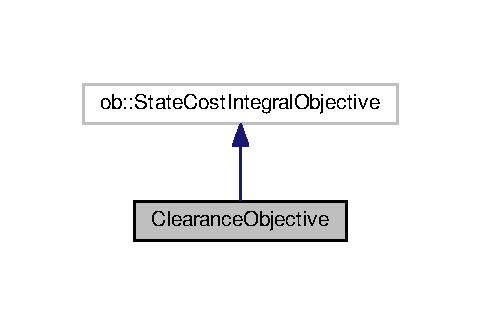
\includegraphics[width=231pt]{classClearanceObjective__inherit__graph}
\end{center}
\end{figure}


Collaboration diagram for Clearance\+Objective\+:\nopagebreak
\begin{figure}[H]
\begin{center}
\leavevmode
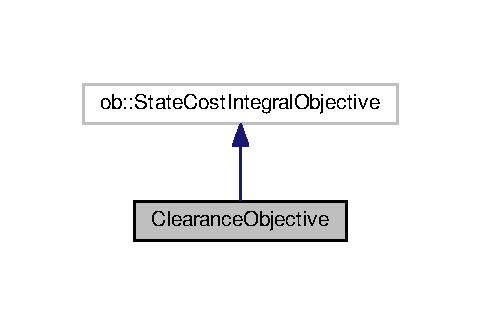
\includegraphics[width=231pt]{classClearanceObjective__coll__graph}
\end{center}
\end{figure}
\subsection*{Public Member Functions}
\begin{DoxyCompactItemize}
\item 
\hyperlink{classClearanceObjective_a168fd22cec3680188f9fd8dbb23661da}{Clearance\+Objective} (const ob\+::\+Space\+Information\+Ptr \&si)
\item 
ob\+::\+Cost \hyperlink{classClearanceObjective_a89162d6d3c598d323d962a2a5c510b6c}{state\+Cost} (const ob\+::\+State $\ast$s) const override
\end{DoxyCompactItemize}


\subsection{Constructor \& Destructor Documentation}
\index{Clearance\+Objective@{Clearance\+Objective}!Clearance\+Objective@{Clearance\+Objective}}
\index{Clearance\+Objective@{Clearance\+Objective}!Clearance\+Objective@{Clearance\+Objective}}
\subsubsection[{\texorpdfstring{Clearance\+Objective(const ob\+::\+Space\+Information\+Ptr \&si)}{ClearanceObjective(const ob::SpaceInformationPtr &si)}}]{\setlength{\rightskip}{0pt plus 5cm}Clearance\+Objective\+::\+Clearance\+Objective (
\begin{DoxyParamCaption}
\item[{const ob\+::\+Space\+Information\+Ptr \&}]{si}
\end{DoxyParamCaption}
)\hspace{0.3cm}{\ttfamily [inline]}}\hypertarget{classClearanceObjective_a168fd22cec3680188f9fd8dbb23661da}{}\label{classClearanceObjective_a168fd22cec3680188f9fd8dbb23661da}


\subsection{Member Function Documentation}
\index{Clearance\+Objective@{Clearance\+Objective}!state\+Cost@{state\+Cost}}
\index{state\+Cost@{state\+Cost}!Clearance\+Objective@{Clearance\+Objective}}
\subsubsection[{\texorpdfstring{state\+Cost(const ob\+::\+State $\ast$s) const override}{stateCost(const ob::State *s) const override}}]{\setlength{\rightskip}{0pt plus 5cm}ob\+::\+Cost Clearance\+Objective\+::state\+Cost (
\begin{DoxyParamCaption}
\item[{const ob\+::\+State $\ast$}]{s}
\end{DoxyParamCaption}
) const\hspace{0.3cm}{\ttfamily [inline]}, {\ttfamily [override]}}\hypertarget{classClearanceObjective_a89162d6d3c598d323d962a2a5c510b6c}{}\label{classClearanceObjective_a89162d6d3c598d323d962a2a5c510b6c}


The documentation for this class was generated from the following file\+:\begin{DoxyCompactItemize}
\item 
include/\hyperlink{ompl__planning_8hpp}{ompl\+\_\+planning.\+hpp}\end{DoxyCompactItemize}

\hypertarget{classconfig__Params__planPath}{}\section{config\+\_\+\+Params\+\_\+plan\+Path Class Reference}
\label{classconfig__Params__planPath}\index{config\+\_\+\+Params\+\_\+plan\+Path@{config\+\_\+\+Params\+\_\+plan\+Path}}


Class which reads and stores the configuration params related to plan\+Path functions.  


\subsection*{Public Member Functions}
\begin{DoxyCompactItemize}
\item 
void \hyperlink{classconfig__Params__planPath_aa0450f0e52f8134af81358873a9cca4b}{read} (const std\+::string \&\hyperlink{classconfig__Params__planPath_a03290d421ed527b13a4caed9caec2de8}{config\+\_\+folder})
\begin{DoxyCompactList}\small\item\em read all params from config file and assign it to class variables \end{DoxyCompactList}\end{DoxyCompactItemize}
\subsection*{Public Attributes}
\begin{DoxyCompactItemize}
\item 
int \hyperlink{classconfig__Params__planPath_a26329f440ce13957ff4c7fb643b66ced}{rrts\+\_\+scaling\+\_\+factor}
\item 
double \hyperlink{classconfig__Params__planPath_a5d43faedc443b4ff25dc2fd5fd27b2dd}{rrts\+\_\+step\+\_\+size}
\item 
int \hyperlink{classconfig__Params__planPath_ade92a1a5f3d29658d460057219f80486}{rrts\+\_\+max\+\_\+iter}
\item 
double \hyperlink{classconfig__Params__planPath_ab021000cd2770f4f9202396dda3aeff7}{rrts\+\_\+goal\+\_\+bias}
\item 
double \hyperlink{classconfig__Params__planPath_af0f84d366ab29443178fb55aa80ac23b}{rrts\+\_\+turn\+\_\+radius}
\item 
double \hyperlink{classconfig__Params__planPath_ab71b5c9e559f89ddea075e8012499d18}{rrts\+\_\+neighbour\+\_\+factor}
\item 
double \hyperlink{classconfig__Params__planPath_aeb42cb9ee0112f1bdee15ff8d5808958}{rrtsompl\+\_\+max\+\_\+solve\+\_\+time}
\item 
int \hyperlink{classconfig__Params__planPath_afee977505c0e321629da095f9f0f91af}{rrtsompl\+\_\+planner\+\_\+type}
\item 
bool \hyperlink{classconfig__Params__planPath_ad95f059b3b5a19b938a4b4bcbff73eab}{use\+\_\+rrt}
\item 
bool \hyperlink{classconfig__Params__planPath_a88d2ed829eea295da08035b2e337a034}{use\+\_\+rrt\+\_\+star}
\item 
bool \hyperlink{classconfig__Params__planPath_a75a7e08f13b232240c5e6a226e34f333}{use\+\_\+rrt\+\_\+star\+\_\+ompl}
\item 
int \hyperlink{classconfig__Params__planPath_a43c04821b004c31011e72c10a250b942}{border\+\_\+radius}
\item 
int \hyperlink{classconfig__Params__planPath_a8d467a6cae6f3afb4d3a628ea7ffa81c}{mission}
\item 
double \hyperlink{classconfig__Params__planPath_a4cde1927f911cd41b43b66668dda3ec9}{mission2\+\_\+threshold\+\_\+distance}
\item 
bool \hyperlink{classconfig__Params__planPath_a6ec518fae1a865e277b6807e87cd71b2}{save\+\_\+global\+\_\+path}
\item 
bool \hyperlink{classconfig__Params__planPath_ad7cdfaff92a0b04065934dc7e9f7bbbf}{save\+\_\+local\+\_\+path}
\item 
string \hyperlink{classconfig__Params__planPath_a7ab6118cdf2af9992ef481d1bc9d965f}{save\+\_\+path\+\_\+location}
\item 
string \hyperlink{classconfig__Params__planPath_a0cbbbf9e0e0830dcb6afc10ebc9d5ba6}{global\+\_\+path\+\_\+file}
\item 
string \hyperlink{classconfig__Params__planPath_a6d7eb54d97fd5e214392294649c867ae}{local\+\_\+path\+\_\+file}
\item 
int \hyperlink{classconfig__Params__planPath_addae22cbaa95dc14ffb3ec6079d21876}{offset\+\_\+radius}
\item 
bool \hyperlink{classconfig__Params__planPath_a3c4ddb466218ec03c2e5e94d6471f730}{use\+\_\+clothoids}
\item 
int \hyperlink{classconfig__Params__planPath_a9a0611f65bd2d57d59c25535c2a7f9b7}{kmax}
\item 
int \hyperlink{classconfig__Params__planPath_ac17efdb44431285cb264482c8e9f2007}{npts}
\item 
double \hyperlink{classconfig__Params__planPath_a782ea20dcd395fbc673bb8145b09dd9f}{dist\+\_\+bet\+\_\+points}
\item 
string \hyperlink{classconfig__Params__planPath_a03290d421ed527b13a4caed9caec2de8}{config\+\_\+folder}
\end{DoxyCompactItemize}


\subsection{Detailed Description}
Class which reads and stores the configuration params related to plan\+Path functions. 

\subsection{Member Function Documentation}
\index{config\+\_\+\+Params\+\_\+plan\+Path@{config\+\_\+\+Params\+\_\+plan\+Path}!read@{read}}
\index{read@{read}!config\+\_\+\+Params\+\_\+plan\+Path@{config\+\_\+\+Params\+\_\+plan\+Path}}
\subsubsection[{\texorpdfstring{read(const std\+::string \&config\+\_\+folder)}{read(const std::string &config_folder)}}]{\setlength{\rightskip}{0pt plus 5cm}void config\+\_\+\+Params\+\_\+plan\+Path\+::read (
\begin{DoxyParamCaption}
\item[{const std\+::string \&}]{config\+\_\+folder}
\end{DoxyParamCaption}
)\hspace{0.3cm}{\ttfamily [inline]}}\hypertarget{classconfig__Params__planPath_aa0450f0e52f8134af81358873a9cca4b}{}\label{classconfig__Params__planPath_aa0450f0e52f8134af81358873a9cca4b}


read all params from config file and assign it to class variables 


\begin{DoxyParams}{Parameters}
{\em config\+\_\+folder} & config folder where the params are available \\
\hline
\end{DoxyParams}


\subsection{Member Data Documentation}
\index{config\+\_\+\+Params\+\_\+plan\+Path@{config\+\_\+\+Params\+\_\+plan\+Path}!border\+\_\+radius@{border\+\_\+radius}}
\index{border\+\_\+radius@{border\+\_\+radius}!config\+\_\+\+Params\+\_\+plan\+Path@{config\+\_\+\+Params\+\_\+plan\+Path}}
\subsubsection[{\texorpdfstring{border\+\_\+radius}{border_radius}}]{\setlength{\rightskip}{0pt plus 5cm}int config\+\_\+\+Params\+\_\+plan\+Path\+::border\+\_\+radius}\hypertarget{classconfig__Params__planPath_a43c04821b004c31011e72c10a250b942}{}\label{classconfig__Params__planPath_a43c04821b004c31011e72c10a250b942}
\index{config\+\_\+\+Params\+\_\+plan\+Path@{config\+\_\+\+Params\+\_\+plan\+Path}!config\+\_\+folder@{config\+\_\+folder}}
\index{config\+\_\+folder@{config\+\_\+folder}!config\+\_\+\+Params\+\_\+plan\+Path@{config\+\_\+\+Params\+\_\+plan\+Path}}
\subsubsection[{\texorpdfstring{config\+\_\+folder}{config_folder}}]{\setlength{\rightskip}{0pt plus 5cm}string config\+\_\+\+Params\+\_\+plan\+Path\+::config\+\_\+folder}\hypertarget{classconfig__Params__planPath_a03290d421ed527b13a4caed9caec2de8}{}\label{classconfig__Params__planPath_a03290d421ed527b13a4caed9caec2de8}
\index{config\+\_\+\+Params\+\_\+plan\+Path@{config\+\_\+\+Params\+\_\+plan\+Path}!dist\+\_\+bet\+\_\+points@{dist\+\_\+bet\+\_\+points}}
\index{dist\+\_\+bet\+\_\+points@{dist\+\_\+bet\+\_\+points}!config\+\_\+\+Params\+\_\+plan\+Path@{config\+\_\+\+Params\+\_\+plan\+Path}}
\subsubsection[{\texorpdfstring{dist\+\_\+bet\+\_\+points}{dist_bet_points}}]{\setlength{\rightskip}{0pt plus 5cm}double config\+\_\+\+Params\+\_\+plan\+Path\+::dist\+\_\+bet\+\_\+points}\hypertarget{classconfig__Params__planPath_a782ea20dcd395fbc673bb8145b09dd9f}{}\label{classconfig__Params__planPath_a782ea20dcd395fbc673bb8145b09dd9f}
\index{config\+\_\+\+Params\+\_\+plan\+Path@{config\+\_\+\+Params\+\_\+plan\+Path}!global\+\_\+path\+\_\+file@{global\+\_\+path\+\_\+file}}
\index{global\+\_\+path\+\_\+file@{global\+\_\+path\+\_\+file}!config\+\_\+\+Params\+\_\+plan\+Path@{config\+\_\+\+Params\+\_\+plan\+Path}}
\subsubsection[{\texorpdfstring{global\+\_\+path\+\_\+file}{global_path_file}}]{\setlength{\rightskip}{0pt plus 5cm}string config\+\_\+\+Params\+\_\+plan\+Path\+::global\+\_\+path\+\_\+file}\hypertarget{classconfig__Params__planPath_a0cbbbf9e0e0830dcb6afc10ebc9d5ba6}{}\label{classconfig__Params__planPath_a0cbbbf9e0e0830dcb6afc10ebc9d5ba6}
\index{config\+\_\+\+Params\+\_\+plan\+Path@{config\+\_\+\+Params\+\_\+plan\+Path}!kmax@{kmax}}
\index{kmax@{kmax}!config\+\_\+\+Params\+\_\+plan\+Path@{config\+\_\+\+Params\+\_\+plan\+Path}}
\subsubsection[{\texorpdfstring{kmax}{kmax}}]{\setlength{\rightskip}{0pt plus 5cm}int config\+\_\+\+Params\+\_\+plan\+Path\+::kmax}\hypertarget{classconfig__Params__planPath_a9a0611f65bd2d57d59c25535c2a7f9b7}{}\label{classconfig__Params__planPath_a9a0611f65bd2d57d59c25535c2a7f9b7}
\index{config\+\_\+\+Params\+\_\+plan\+Path@{config\+\_\+\+Params\+\_\+plan\+Path}!local\+\_\+path\+\_\+file@{local\+\_\+path\+\_\+file}}
\index{local\+\_\+path\+\_\+file@{local\+\_\+path\+\_\+file}!config\+\_\+\+Params\+\_\+plan\+Path@{config\+\_\+\+Params\+\_\+plan\+Path}}
\subsubsection[{\texorpdfstring{local\+\_\+path\+\_\+file}{local_path_file}}]{\setlength{\rightskip}{0pt plus 5cm}string config\+\_\+\+Params\+\_\+plan\+Path\+::local\+\_\+path\+\_\+file}\hypertarget{classconfig__Params__planPath_a6d7eb54d97fd5e214392294649c867ae}{}\label{classconfig__Params__planPath_a6d7eb54d97fd5e214392294649c867ae}
\index{config\+\_\+\+Params\+\_\+plan\+Path@{config\+\_\+\+Params\+\_\+plan\+Path}!mission@{mission}}
\index{mission@{mission}!config\+\_\+\+Params\+\_\+plan\+Path@{config\+\_\+\+Params\+\_\+plan\+Path}}
\subsubsection[{\texorpdfstring{mission}{mission}}]{\setlength{\rightskip}{0pt plus 5cm}int config\+\_\+\+Params\+\_\+plan\+Path\+::mission}\hypertarget{classconfig__Params__planPath_a8d467a6cae6f3afb4d3a628ea7ffa81c}{}\label{classconfig__Params__planPath_a8d467a6cae6f3afb4d3a628ea7ffa81c}
\index{config\+\_\+\+Params\+\_\+plan\+Path@{config\+\_\+\+Params\+\_\+plan\+Path}!mission2\+\_\+threshold\+\_\+distance@{mission2\+\_\+threshold\+\_\+distance}}
\index{mission2\+\_\+threshold\+\_\+distance@{mission2\+\_\+threshold\+\_\+distance}!config\+\_\+\+Params\+\_\+plan\+Path@{config\+\_\+\+Params\+\_\+plan\+Path}}
\subsubsection[{\texorpdfstring{mission2\+\_\+threshold\+\_\+distance}{mission2_threshold_distance}}]{\setlength{\rightskip}{0pt plus 5cm}double config\+\_\+\+Params\+\_\+plan\+Path\+::mission2\+\_\+threshold\+\_\+distance}\hypertarget{classconfig__Params__planPath_a4cde1927f911cd41b43b66668dda3ec9}{}\label{classconfig__Params__planPath_a4cde1927f911cd41b43b66668dda3ec9}
\index{config\+\_\+\+Params\+\_\+plan\+Path@{config\+\_\+\+Params\+\_\+plan\+Path}!npts@{npts}}
\index{npts@{npts}!config\+\_\+\+Params\+\_\+plan\+Path@{config\+\_\+\+Params\+\_\+plan\+Path}}
\subsubsection[{\texorpdfstring{npts}{npts}}]{\setlength{\rightskip}{0pt plus 5cm}int config\+\_\+\+Params\+\_\+plan\+Path\+::npts}\hypertarget{classconfig__Params__planPath_ac17efdb44431285cb264482c8e9f2007}{}\label{classconfig__Params__planPath_ac17efdb44431285cb264482c8e9f2007}
\index{config\+\_\+\+Params\+\_\+plan\+Path@{config\+\_\+\+Params\+\_\+plan\+Path}!offset\+\_\+radius@{offset\+\_\+radius}}
\index{offset\+\_\+radius@{offset\+\_\+radius}!config\+\_\+\+Params\+\_\+plan\+Path@{config\+\_\+\+Params\+\_\+plan\+Path}}
\subsubsection[{\texorpdfstring{offset\+\_\+radius}{offset_radius}}]{\setlength{\rightskip}{0pt plus 5cm}int config\+\_\+\+Params\+\_\+plan\+Path\+::offset\+\_\+radius}\hypertarget{classconfig__Params__planPath_addae22cbaa95dc14ffb3ec6079d21876}{}\label{classconfig__Params__planPath_addae22cbaa95dc14ffb3ec6079d21876}
\index{config\+\_\+\+Params\+\_\+plan\+Path@{config\+\_\+\+Params\+\_\+plan\+Path}!rrts\+\_\+goal\+\_\+bias@{rrts\+\_\+goal\+\_\+bias}}
\index{rrts\+\_\+goal\+\_\+bias@{rrts\+\_\+goal\+\_\+bias}!config\+\_\+\+Params\+\_\+plan\+Path@{config\+\_\+\+Params\+\_\+plan\+Path}}
\subsubsection[{\texorpdfstring{rrts\+\_\+goal\+\_\+bias}{rrts_goal_bias}}]{\setlength{\rightskip}{0pt plus 5cm}double config\+\_\+\+Params\+\_\+plan\+Path\+::rrts\+\_\+goal\+\_\+bias}\hypertarget{classconfig__Params__planPath_ab021000cd2770f4f9202396dda3aeff7}{}\label{classconfig__Params__planPath_ab021000cd2770f4f9202396dda3aeff7}
\index{config\+\_\+\+Params\+\_\+plan\+Path@{config\+\_\+\+Params\+\_\+plan\+Path}!rrts\+\_\+max\+\_\+iter@{rrts\+\_\+max\+\_\+iter}}
\index{rrts\+\_\+max\+\_\+iter@{rrts\+\_\+max\+\_\+iter}!config\+\_\+\+Params\+\_\+plan\+Path@{config\+\_\+\+Params\+\_\+plan\+Path}}
\subsubsection[{\texorpdfstring{rrts\+\_\+max\+\_\+iter}{rrts_max_iter}}]{\setlength{\rightskip}{0pt plus 5cm}int config\+\_\+\+Params\+\_\+plan\+Path\+::rrts\+\_\+max\+\_\+iter}\hypertarget{classconfig__Params__planPath_ade92a1a5f3d29658d460057219f80486}{}\label{classconfig__Params__planPath_ade92a1a5f3d29658d460057219f80486}
\index{config\+\_\+\+Params\+\_\+plan\+Path@{config\+\_\+\+Params\+\_\+plan\+Path}!rrts\+\_\+neighbour\+\_\+factor@{rrts\+\_\+neighbour\+\_\+factor}}
\index{rrts\+\_\+neighbour\+\_\+factor@{rrts\+\_\+neighbour\+\_\+factor}!config\+\_\+\+Params\+\_\+plan\+Path@{config\+\_\+\+Params\+\_\+plan\+Path}}
\subsubsection[{\texorpdfstring{rrts\+\_\+neighbour\+\_\+factor}{rrts_neighbour_factor}}]{\setlength{\rightskip}{0pt plus 5cm}double config\+\_\+\+Params\+\_\+plan\+Path\+::rrts\+\_\+neighbour\+\_\+factor}\hypertarget{classconfig__Params__planPath_ab71b5c9e559f89ddea075e8012499d18}{}\label{classconfig__Params__planPath_ab71b5c9e559f89ddea075e8012499d18}
\index{config\+\_\+\+Params\+\_\+plan\+Path@{config\+\_\+\+Params\+\_\+plan\+Path}!rrts\+\_\+scaling\+\_\+factor@{rrts\+\_\+scaling\+\_\+factor}}
\index{rrts\+\_\+scaling\+\_\+factor@{rrts\+\_\+scaling\+\_\+factor}!config\+\_\+\+Params\+\_\+plan\+Path@{config\+\_\+\+Params\+\_\+plan\+Path}}
\subsubsection[{\texorpdfstring{rrts\+\_\+scaling\+\_\+factor}{rrts_scaling_factor}}]{\setlength{\rightskip}{0pt plus 5cm}int config\+\_\+\+Params\+\_\+plan\+Path\+::rrts\+\_\+scaling\+\_\+factor}\hypertarget{classconfig__Params__planPath_a26329f440ce13957ff4c7fb643b66ced}{}\label{classconfig__Params__planPath_a26329f440ce13957ff4c7fb643b66ced}
\index{config\+\_\+\+Params\+\_\+plan\+Path@{config\+\_\+\+Params\+\_\+plan\+Path}!rrts\+\_\+step\+\_\+size@{rrts\+\_\+step\+\_\+size}}
\index{rrts\+\_\+step\+\_\+size@{rrts\+\_\+step\+\_\+size}!config\+\_\+\+Params\+\_\+plan\+Path@{config\+\_\+\+Params\+\_\+plan\+Path}}
\subsubsection[{\texorpdfstring{rrts\+\_\+step\+\_\+size}{rrts_step_size}}]{\setlength{\rightskip}{0pt plus 5cm}double config\+\_\+\+Params\+\_\+plan\+Path\+::rrts\+\_\+step\+\_\+size}\hypertarget{classconfig__Params__planPath_a5d43faedc443b4ff25dc2fd5fd27b2dd}{}\label{classconfig__Params__planPath_a5d43faedc443b4ff25dc2fd5fd27b2dd}
\index{config\+\_\+\+Params\+\_\+plan\+Path@{config\+\_\+\+Params\+\_\+plan\+Path}!rrts\+\_\+turn\+\_\+radius@{rrts\+\_\+turn\+\_\+radius}}
\index{rrts\+\_\+turn\+\_\+radius@{rrts\+\_\+turn\+\_\+radius}!config\+\_\+\+Params\+\_\+plan\+Path@{config\+\_\+\+Params\+\_\+plan\+Path}}
\subsubsection[{\texorpdfstring{rrts\+\_\+turn\+\_\+radius}{rrts_turn_radius}}]{\setlength{\rightskip}{0pt plus 5cm}double config\+\_\+\+Params\+\_\+plan\+Path\+::rrts\+\_\+turn\+\_\+radius}\hypertarget{classconfig__Params__planPath_af0f84d366ab29443178fb55aa80ac23b}{}\label{classconfig__Params__planPath_af0f84d366ab29443178fb55aa80ac23b}
\index{config\+\_\+\+Params\+\_\+plan\+Path@{config\+\_\+\+Params\+\_\+plan\+Path}!rrtsompl\+\_\+max\+\_\+solve\+\_\+time@{rrtsompl\+\_\+max\+\_\+solve\+\_\+time}}
\index{rrtsompl\+\_\+max\+\_\+solve\+\_\+time@{rrtsompl\+\_\+max\+\_\+solve\+\_\+time}!config\+\_\+\+Params\+\_\+plan\+Path@{config\+\_\+\+Params\+\_\+plan\+Path}}
\subsubsection[{\texorpdfstring{rrtsompl\+\_\+max\+\_\+solve\+\_\+time}{rrtsompl_max_solve_time}}]{\setlength{\rightskip}{0pt plus 5cm}double config\+\_\+\+Params\+\_\+plan\+Path\+::rrtsompl\+\_\+max\+\_\+solve\+\_\+time}\hypertarget{classconfig__Params__planPath_aeb42cb9ee0112f1bdee15ff8d5808958}{}\label{classconfig__Params__planPath_aeb42cb9ee0112f1bdee15ff8d5808958}
\index{config\+\_\+\+Params\+\_\+plan\+Path@{config\+\_\+\+Params\+\_\+plan\+Path}!rrtsompl\+\_\+planner\+\_\+type@{rrtsompl\+\_\+planner\+\_\+type}}
\index{rrtsompl\+\_\+planner\+\_\+type@{rrtsompl\+\_\+planner\+\_\+type}!config\+\_\+\+Params\+\_\+plan\+Path@{config\+\_\+\+Params\+\_\+plan\+Path}}
\subsubsection[{\texorpdfstring{rrtsompl\+\_\+planner\+\_\+type}{rrtsompl_planner_type}}]{\setlength{\rightskip}{0pt plus 5cm}int config\+\_\+\+Params\+\_\+plan\+Path\+::rrtsompl\+\_\+planner\+\_\+type}\hypertarget{classconfig__Params__planPath_afee977505c0e321629da095f9f0f91af}{}\label{classconfig__Params__planPath_afee977505c0e321629da095f9f0f91af}
\index{config\+\_\+\+Params\+\_\+plan\+Path@{config\+\_\+\+Params\+\_\+plan\+Path}!save\+\_\+global\+\_\+path@{save\+\_\+global\+\_\+path}}
\index{save\+\_\+global\+\_\+path@{save\+\_\+global\+\_\+path}!config\+\_\+\+Params\+\_\+plan\+Path@{config\+\_\+\+Params\+\_\+plan\+Path}}
\subsubsection[{\texorpdfstring{save\+\_\+global\+\_\+path}{save_global_path}}]{\setlength{\rightskip}{0pt plus 5cm}bool config\+\_\+\+Params\+\_\+plan\+Path\+::save\+\_\+global\+\_\+path}\hypertarget{classconfig__Params__planPath_a6ec518fae1a865e277b6807e87cd71b2}{}\label{classconfig__Params__planPath_a6ec518fae1a865e277b6807e87cd71b2}
\index{config\+\_\+\+Params\+\_\+plan\+Path@{config\+\_\+\+Params\+\_\+plan\+Path}!save\+\_\+local\+\_\+path@{save\+\_\+local\+\_\+path}}
\index{save\+\_\+local\+\_\+path@{save\+\_\+local\+\_\+path}!config\+\_\+\+Params\+\_\+plan\+Path@{config\+\_\+\+Params\+\_\+plan\+Path}}
\subsubsection[{\texorpdfstring{save\+\_\+local\+\_\+path}{save_local_path}}]{\setlength{\rightskip}{0pt plus 5cm}bool config\+\_\+\+Params\+\_\+plan\+Path\+::save\+\_\+local\+\_\+path}\hypertarget{classconfig__Params__planPath_ad7cdfaff92a0b04065934dc7e9f7bbbf}{}\label{classconfig__Params__planPath_ad7cdfaff92a0b04065934dc7e9f7bbbf}
\index{config\+\_\+\+Params\+\_\+plan\+Path@{config\+\_\+\+Params\+\_\+plan\+Path}!save\+\_\+path\+\_\+location@{save\+\_\+path\+\_\+location}}
\index{save\+\_\+path\+\_\+location@{save\+\_\+path\+\_\+location}!config\+\_\+\+Params\+\_\+plan\+Path@{config\+\_\+\+Params\+\_\+plan\+Path}}
\subsubsection[{\texorpdfstring{save\+\_\+path\+\_\+location}{save_path_location}}]{\setlength{\rightskip}{0pt plus 5cm}string config\+\_\+\+Params\+\_\+plan\+Path\+::save\+\_\+path\+\_\+location}\hypertarget{classconfig__Params__planPath_a7ab6118cdf2af9992ef481d1bc9d965f}{}\label{classconfig__Params__planPath_a7ab6118cdf2af9992ef481d1bc9d965f}
\index{config\+\_\+\+Params\+\_\+plan\+Path@{config\+\_\+\+Params\+\_\+plan\+Path}!use\+\_\+clothoids@{use\+\_\+clothoids}}
\index{use\+\_\+clothoids@{use\+\_\+clothoids}!config\+\_\+\+Params\+\_\+plan\+Path@{config\+\_\+\+Params\+\_\+plan\+Path}}
\subsubsection[{\texorpdfstring{use\+\_\+clothoids}{use_clothoids}}]{\setlength{\rightskip}{0pt plus 5cm}bool config\+\_\+\+Params\+\_\+plan\+Path\+::use\+\_\+clothoids}\hypertarget{classconfig__Params__planPath_a3c4ddb466218ec03c2e5e94d6471f730}{}\label{classconfig__Params__planPath_a3c4ddb466218ec03c2e5e94d6471f730}
\index{config\+\_\+\+Params\+\_\+plan\+Path@{config\+\_\+\+Params\+\_\+plan\+Path}!use\+\_\+rrt@{use\+\_\+rrt}}
\index{use\+\_\+rrt@{use\+\_\+rrt}!config\+\_\+\+Params\+\_\+plan\+Path@{config\+\_\+\+Params\+\_\+plan\+Path}}
\subsubsection[{\texorpdfstring{use\+\_\+rrt}{use_rrt}}]{\setlength{\rightskip}{0pt plus 5cm}bool config\+\_\+\+Params\+\_\+plan\+Path\+::use\+\_\+rrt}\hypertarget{classconfig__Params__planPath_ad95f059b3b5a19b938a4b4bcbff73eab}{}\label{classconfig__Params__planPath_ad95f059b3b5a19b938a4b4bcbff73eab}
\index{config\+\_\+\+Params\+\_\+plan\+Path@{config\+\_\+\+Params\+\_\+plan\+Path}!use\+\_\+rrt\+\_\+star@{use\+\_\+rrt\+\_\+star}}
\index{use\+\_\+rrt\+\_\+star@{use\+\_\+rrt\+\_\+star}!config\+\_\+\+Params\+\_\+plan\+Path@{config\+\_\+\+Params\+\_\+plan\+Path}}
\subsubsection[{\texorpdfstring{use\+\_\+rrt\+\_\+star}{use_rrt_star}}]{\setlength{\rightskip}{0pt plus 5cm}bool config\+\_\+\+Params\+\_\+plan\+Path\+::use\+\_\+rrt\+\_\+star}\hypertarget{classconfig__Params__planPath_a88d2ed829eea295da08035b2e337a034}{}\label{classconfig__Params__planPath_a88d2ed829eea295da08035b2e337a034}
\index{config\+\_\+\+Params\+\_\+plan\+Path@{config\+\_\+\+Params\+\_\+plan\+Path}!use\+\_\+rrt\+\_\+star\+\_\+ompl@{use\+\_\+rrt\+\_\+star\+\_\+ompl}}
\index{use\+\_\+rrt\+\_\+star\+\_\+ompl@{use\+\_\+rrt\+\_\+star\+\_\+ompl}!config\+\_\+\+Params\+\_\+plan\+Path@{config\+\_\+\+Params\+\_\+plan\+Path}}
\subsubsection[{\texorpdfstring{use\+\_\+rrt\+\_\+star\+\_\+ompl}{use_rrt_star_ompl}}]{\setlength{\rightskip}{0pt plus 5cm}bool config\+\_\+\+Params\+\_\+plan\+Path\+::use\+\_\+rrt\+\_\+star\+\_\+ompl}\hypertarget{classconfig__Params__planPath_a75a7e08f13b232240c5e6a226e34f333}{}\label{classconfig__Params__planPath_a75a7e08f13b232240c5e6a226e34f333}


The documentation for this class was generated from the following file\+:\begin{DoxyCompactItemize}
\item 
src/\hyperlink{planPath_8cpp}{plan\+Path.\+cpp}\end{DoxyCompactItemize}

\hypertarget{classconfig__Params__ProcessMap}{}\section{config\+\_\+\+Params\+\_\+\+Process\+Map Class Reference}
\label{classconfig__Params__ProcessMap}\index{config\+\_\+\+Params\+\_\+\+Process\+Map@{config\+\_\+\+Params\+\_\+\+Process\+Map}}


Class which reads and stores the configuration params related to process\+Map functions.  


\subsection*{Public Member Functions}
\begin{DoxyCompactItemize}
\item 
void \hyperlink{classconfig__Params__ProcessMap_a31fb9d4c3cb96147d08e7b313e8e81e3}{read} (const std\+::string \&\hyperlink{classconfig__Params__ProcessMap_a4f13c462c22d1c92513401b800ba5b15}{config\+\_\+folder})
\begin{DoxyCompactList}\small\item\em read all params from config file and assign it to class variables \end{DoxyCompactList}\item 
void \hyperlink{classconfig__Params__ProcessMap_a6c1029c265112fc3337334da05eb1854}{print} ()
\begin{DoxyCompactList}\small\item\em print all params for debug \end{DoxyCompactList}\end{DoxyCompactItemize}
\subsection*{Public Attributes}
\begin{DoxyCompactItemize}
\item 
bool \hyperlink{classconfig__Params__ProcessMap_ae591827a509aec2c225311dff3745500}{find\+\_\+victims\+\_\+debug\+\_\+plot}
\item 
bool \hyperlink{classconfig__Params__ProcessMap_a95ef6dae3b8ea5729474e29ecab73abc}{find\+\_\+gate\+\_\+debug\+\_\+plot}
\item 
bool \hyperlink{classconfig__Params__ProcessMap_a4fd3039d8067dccf1049f5059da136b8}{find\+\_\+obstacles\+\_\+debug\+\_\+plot}
\item 
bool \hyperlink{classconfig__Params__ProcessMap_a839b04d0ee3c03af92f9abf62bdafa5d}{debug\+\_\+victim\+\_\+id}
\item 
bool \hyperlink{classconfig__Params__ProcessMap_a33441b8db8108220849c6b84381a99f7}{use\+\_\+ocr}
\item 
bool \hyperlink{classconfig__Params__ProcessMap_a5bcffdee06a89ee4157bcd524d70b1eb}{use\+\_\+flip}
\item 
string \hyperlink{classconfig__Params__ProcessMap_a4f13c462c22d1c92513401b800ba5b15}{config\+\_\+folder}
\end{DoxyCompactItemize}


\subsection{Detailed Description}
Class which reads and stores the configuration params related to process\+Map functions. 

\subsection{Member Function Documentation}
\index{config\+\_\+\+Params\+\_\+\+Process\+Map@{config\+\_\+\+Params\+\_\+\+Process\+Map}!print@{print}}
\index{print@{print}!config\+\_\+\+Params\+\_\+\+Process\+Map@{config\+\_\+\+Params\+\_\+\+Process\+Map}}
\subsubsection[{\texorpdfstring{print()}{print()}}]{\setlength{\rightskip}{0pt plus 5cm}void config\+\_\+\+Params\+\_\+\+Process\+Map\+::print (
\begin{DoxyParamCaption}
{}
\end{DoxyParamCaption}
)\hspace{0.3cm}{\ttfamily [inline]}}\hypertarget{classconfig__Params__ProcessMap_a6c1029c265112fc3337334da05eb1854}{}\label{classconfig__Params__ProcessMap_a6c1029c265112fc3337334da05eb1854}


print all params for debug 

\index{config\+\_\+\+Params\+\_\+\+Process\+Map@{config\+\_\+\+Params\+\_\+\+Process\+Map}!read@{read}}
\index{read@{read}!config\+\_\+\+Params\+\_\+\+Process\+Map@{config\+\_\+\+Params\+\_\+\+Process\+Map}}
\subsubsection[{\texorpdfstring{read(const std\+::string \&config\+\_\+folder)}{read(const std::string &config_folder)}}]{\setlength{\rightskip}{0pt plus 5cm}void config\+\_\+\+Params\+\_\+\+Process\+Map\+::read (
\begin{DoxyParamCaption}
\item[{const std\+::string \&}]{config\+\_\+folder}
\end{DoxyParamCaption}
)\hspace{0.3cm}{\ttfamily [inline]}}\hypertarget{classconfig__Params__ProcessMap_a31fb9d4c3cb96147d08e7b313e8e81e3}{}\label{classconfig__Params__ProcessMap_a31fb9d4c3cb96147d08e7b313e8e81e3}


read all params from config file and assign it to class variables 


\begin{DoxyParams}{Parameters}
{\em config\+\_\+folder} & config folder where the params are available \\
\hline
\end{DoxyParams}


\subsection{Member Data Documentation}
\index{config\+\_\+\+Params\+\_\+\+Process\+Map@{config\+\_\+\+Params\+\_\+\+Process\+Map}!config\+\_\+folder@{config\+\_\+folder}}
\index{config\+\_\+folder@{config\+\_\+folder}!config\+\_\+\+Params\+\_\+\+Process\+Map@{config\+\_\+\+Params\+\_\+\+Process\+Map}}
\subsubsection[{\texorpdfstring{config\+\_\+folder}{config_folder}}]{\setlength{\rightskip}{0pt plus 5cm}string config\+\_\+\+Params\+\_\+\+Process\+Map\+::config\+\_\+folder}\hypertarget{classconfig__Params__ProcessMap_a4f13c462c22d1c92513401b800ba5b15}{}\label{classconfig__Params__ProcessMap_a4f13c462c22d1c92513401b800ba5b15}
Flip the image input image \index{config\+\_\+\+Params\+\_\+\+Process\+Map@{config\+\_\+\+Params\+\_\+\+Process\+Map}!debug\+\_\+victim\+\_\+id@{debug\+\_\+victim\+\_\+id}}
\index{debug\+\_\+victim\+\_\+id@{debug\+\_\+victim\+\_\+id}!config\+\_\+\+Params\+\_\+\+Process\+Map@{config\+\_\+\+Params\+\_\+\+Process\+Map}}
\subsubsection[{\texorpdfstring{debug\+\_\+victim\+\_\+id}{debug_victim_id}}]{\setlength{\rightskip}{0pt plus 5cm}bool config\+\_\+\+Params\+\_\+\+Process\+Map\+::debug\+\_\+victim\+\_\+id}\hypertarget{classconfig__Params__ProcessMap_a839b04d0ee3c03af92f9abf62bdafa5d}{}\label{classconfig__Params__ProcessMap_a839b04d0ee3c03af92f9abf62bdafa5d}
variable for obstacle debug \index{config\+\_\+\+Params\+\_\+\+Process\+Map@{config\+\_\+\+Params\+\_\+\+Process\+Map}!find\+\_\+gate\+\_\+debug\+\_\+plot@{find\+\_\+gate\+\_\+debug\+\_\+plot}}
\index{find\+\_\+gate\+\_\+debug\+\_\+plot@{find\+\_\+gate\+\_\+debug\+\_\+plot}!config\+\_\+\+Params\+\_\+\+Process\+Map@{config\+\_\+\+Params\+\_\+\+Process\+Map}}
\subsubsection[{\texorpdfstring{find\+\_\+gate\+\_\+debug\+\_\+plot}{find_gate_debug_plot}}]{\setlength{\rightskip}{0pt plus 5cm}bool config\+\_\+\+Params\+\_\+\+Process\+Map\+::find\+\_\+gate\+\_\+debug\+\_\+plot}\hypertarget{classconfig__Params__ProcessMap_a95ef6dae3b8ea5729474e29ecab73abc}{}\label{classconfig__Params__ProcessMap_a95ef6dae3b8ea5729474e29ecab73abc}
variable for victim debug \index{config\+\_\+\+Params\+\_\+\+Process\+Map@{config\+\_\+\+Params\+\_\+\+Process\+Map}!find\+\_\+obstacles\+\_\+debug\+\_\+plot@{find\+\_\+obstacles\+\_\+debug\+\_\+plot}}
\index{find\+\_\+obstacles\+\_\+debug\+\_\+plot@{find\+\_\+obstacles\+\_\+debug\+\_\+plot}!config\+\_\+\+Params\+\_\+\+Process\+Map@{config\+\_\+\+Params\+\_\+\+Process\+Map}}
\subsubsection[{\texorpdfstring{find\+\_\+obstacles\+\_\+debug\+\_\+plot}{find_obstacles_debug_plot}}]{\setlength{\rightskip}{0pt plus 5cm}bool config\+\_\+\+Params\+\_\+\+Process\+Map\+::find\+\_\+obstacles\+\_\+debug\+\_\+plot}\hypertarget{classconfig__Params__ProcessMap_a4fd3039d8067dccf1049f5059da136b8}{}\label{classconfig__Params__ProcessMap_a4fd3039d8067dccf1049f5059da136b8}
variable for gate debug \index{config\+\_\+\+Params\+\_\+\+Process\+Map@{config\+\_\+\+Params\+\_\+\+Process\+Map}!find\+\_\+victims\+\_\+debug\+\_\+plot@{find\+\_\+victims\+\_\+debug\+\_\+plot}}
\index{find\+\_\+victims\+\_\+debug\+\_\+plot@{find\+\_\+victims\+\_\+debug\+\_\+plot}!config\+\_\+\+Params\+\_\+\+Process\+Map@{config\+\_\+\+Params\+\_\+\+Process\+Map}}
\subsubsection[{\texorpdfstring{find\+\_\+victims\+\_\+debug\+\_\+plot}{find_victims_debug_plot}}]{\setlength{\rightskip}{0pt plus 5cm}bool config\+\_\+\+Params\+\_\+\+Process\+Map\+::find\+\_\+victims\+\_\+debug\+\_\+plot}\hypertarget{classconfig__Params__ProcessMap_ae591827a509aec2c225311dff3745500}{}\label{classconfig__Params__ProcessMap_ae591827a509aec2c225311dff3745500}
\index{config\+\_\+\+Params\+\_\+\+Process\+Map@{config\+\_\+\+Params\+\_\+\+Process\+Map}!use\+\_\+flip@{use\+\_\+flip}}
\index{use\+\_\+flip@{use\+\_\+flip}!config\+\_\+\+Params\+\_\+\+Process\+Map@{config\+\_\+\+Params\+\_\+\+Process\+Map}}
\subsubsection[{\texorpdfstring{use\+\_\+flip}{use_flip}}]{\setlength{\rightskip}{0pt plus 5cm}bool config\+\_\+\+Params\+\_\+\+Process\+Map\+::use\+\_\+flip}\hypertarget{classconfig__Params__ProcessMap_a5bcffdee06a89ee4157bcd524d70b1eb}{}\label{classconfig__Params__ProcessMap_a5bcffdee06a89ee4157bcd524d70b1eb}
O\+CR method of detection \index{config\+\_\+\+Params\+\_\+\+Process\+Map@{config\+\_\+\+Params\+\_\+\+Process\+Map}!use\+\_\+ocr@{use\+\_\+ocr}}
\index{use\+\_\+ocr@{use\+\_\+ocr}!config\+\_\+\+Params\+\_\+\+Process\+Map@{config\+\_\+\+Params\+\_\+\+Process\+Map}}
\subsubsection[{\texorpdfstring{use\+\_\+ocr}{use_ocr}}]{\setlength{\rightskip}{0pt plus 5cm}bool config\+\_\+\+Params\+\_\+\+Process\+Map\+::use\+\_\+ocr}\hypertarget{classconfig__Params__ProcessMap_a33441b8db8108220849c6b84381a99f7}{}\label{classconfig__Params__ProcessMap_a33441b8db8108220849c6b84381a99f7}
variable for victim id recognition debug 

The documentation for this class was generated from the following file\+:\begin{DoxyCompactItemize}
\item 
src/\hyperlink{processMap_8cpp}{process\+Map.\+cpp}\end{DoxyCompactItemize}

\hypertarget{structdubinsArc}{}\section{dubins\+Arc Struct Reference}
\label{structdubinsArc}\index{dubins\+Arc@{dubins\+Arc}}


Structure for a Dubins arc  




{\ttfamily \#include $<$dubins\+\_\+local.\+h$>$}

\subsection*{Public Attributes}
\begin{DoxyCompactItemize}
\item 
double \hyperlink{structdubinsArc_a120eba56ab37025c4de0835b90a3faf2}{x0}
\item 
double \hyperlink{structdubinsArc_ae05a57a66703e9993a68c23160a7b54a}{y0}
\item 
double \hyperlink{structdubinsArc_a51bb953226e122a68b132cd4c7d4a198}{th0}
\item 
double \hyperlink{structdubinsArc_ae3556ac95899f6a96dcb728a864c74b3}{k}
\item 
double \hyperlink{structdubinsArc_a5fe3bc6759fc84ee91d254c84015d34d}{s}
\item 
double \hyperlink{structdubinsArc_a5bad303217c1f05eb0feb97d9b636528}{xf}
\item 
double \hyperlink{structdubinsArc_a782cb717a7d9ab1836d3fae17073f104}{yf}
\item 
double \hyperlink{structdubinsArc_aca32bb174d947ee2e38fc00dda92bc63}{thf}
\end{DoxyCompactItemize}


\subsection{Detailed Description}
Structure for a Dubins arc 

\subsection{Member Data Documentation}
\index{dubins\+Arc@{dubins\+Arc}!k@{k}}
\index{k@{k}!dubins\+Arc@{dubins\+Arc}}
\subsubsection[{\texorpdfstring{k}{k}}]{\setlength{\rightskip}{0pt plus 5cm}double dubins\+Arc\+::k}\hypertarget{structdubinsArc_ae3556ac95899f6a96dcb728a864c74b3}{}\label{structdubinsArc_ae3556ac95899f6a96dcb728a864c74b3}
\index{dubins\+Arc@{dubins\+Arc}!s@{s}}
\index{s@{s}!dubins\+Arc@{dubins\+Arc}}
\subsubsection[{\texorpdfstring{s}{s}}]{\setlength{\rightskip}{0pt plus 5cm}double dubins\+Arc\+::s}\hypertarget{structdubinsArc_a5fe3bc6759fc84ee91d254c84015d34d}{}\label{structdubinsArc_a5fe3bc6759fc84ee91d254c84015d34d}
\index{dubins\+Arc@{dubins\+Arc}!th0@{th0}}
\index{th0@{th0}!dubins\+Arc@{dubins\+Arc}}
\subsubsection[{\texorpdfstring{th0}{th0}}]{\setlength{\rightskip}{0pt plus 5cm}double dubins\+Arc\+::th0}\hypertarget{structdubinsArc_a51bb953226e122a68b132cd4c7d4a198}{}\label{structdubinsArc_a51bb953226e122a68b132cd4c7d4a198}
\index{dubins\+Arc@{dubins\+Arc}!thf@{thf}}
\index{thf@{thf}!dubins\+Arc@{dubins\+Arc}}
\subsubsection[{\texorpdfstring{thf}{thf}}]{\setlength{\rightskip}{0pt plus 5cm}double dubins\+Arc\+::thf}\hypertarget{structdubinsArc_aca32bb174d947ee2e38fc00dda92bc63}{}\label{structdubinsArc_aca32bb174d947ee2e38fc00dda92bc63}
\index{dubins\+Arc@{dubins\+Arc}!x0@{x0}}
\index{x0@{x0}!dubins\+Arc@{dubins\+Arc}}
\subsubsection[{\texorpdfstring{x0}{x0}}]{\setlength{\rightskip}{0pt plus 5cm}double dubins\+Arc\+::x0}\hypertarget{structdubinsArc_a120eba56ab37025c4de0835b90a3faf2}{}\label{structdubinsArc_a120eba56ab37025c4de0835b90a3faf2}
\index{dubins\+Arc@{dubins\+Arc}!xf@{xf}}
\index{xf@{xf}!dubins\+Arc@{dubins\+Arc}}
\subsubsection[{\texorpdfstring{xf}{xf}}]{\setlength{\rightskip}{0pt plus 5cm}double dubins\+Arc\+::xf}\hypertarget{structdubinsArc_a5bad303217c1f05eb0feb97d9b636528}{}\label{structdubinsArc_a5bad303217c1f05eb0feb97d9b636528}
\index{dubins\+Arc@{dubins\+Arc}!y0@{y0}}
\index{y0@{y0}!dubins\+Arc@{dubins\+Arc}}
\subsubsection[{\texorpdfstring{y0}{y0}}]{\setlength{\rightskip}{0pt plus 5cm}double dubins\+Arc\+::y0}\hypertarget{structdubinsArc_ae05a57a66703e9993a68c23160a7b54a}{}\label{structdubinsArc_ae05a57a66703e9993a68c23160a7b54a}
\index{dubins\+Arc@{dubins\+Arc}!yf@{yf}}
\index{yf@{yf}!dubins\+Arc@{dubins\+Arc}}
\subsubsection[{\texorpdfstring{yf}{yf}}]{\setlength{\rightskip}{0pt plus 5cm}double dubins\+Arc\+::yf}\hypertarget{structdubinsArc_a782cb717a7d9ab1836d3fae17073f104}{}\label{structdubinsArc_a782cb717a7d9ab1836d3fae17073f104}


The documentation for this struct was generated from the following file\+:\begin{DoxyCompactItemize}
\item 
include/\hyperlink{dubins__local_8h}{dubins\+\_\+local.\+h}\end{DoxyCompactItemize}

\hypertarget{structdubinsCurve}{}\section{dubins\+Curve Struct Reference}
\label{structdubinsCurve}\index{dubins\+Curve@{dubins\+Curve}}


Structure for a Dubins curve.  




{\ttfamily \#include $<$dubins\+\_\+local.\+h$>$}



Collaboration diagram for dubins\+Curve\+:\nopagebreak
\begin{figure}[H]
\begin{center}
\leavevmode
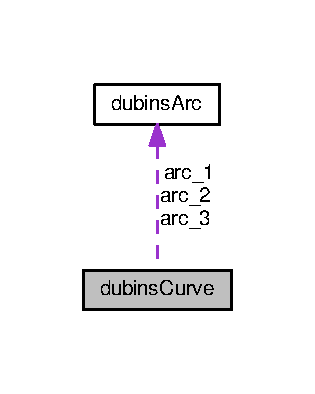
\includegraphics[width=151pt]{structdubinsCurve__coll__graph}
\end{center}
\end{figure}
\subsection*{Public Attributes}
\begin{DoxyCompactItemize}
\item 
\hyperlink{structdubinsArc}{dubins\+Arc} \hyperlink{structdubinsCurve_a0a21df61b2cb1cdd397bdc54b5aa7d7a}{arc\+\_\+1}
\item 
\hyperlink{structdubinsArc}{dubins\+Arc} \hyperlink{structdubinsCurve_ac1cfde797f443b1a73ec3786bcc05e1e}{arc\+\_\+2}
\item 
\hyperlink{structdubinsArc}{dubins\+Arc} \hyperlink{structdubinsCurve_a523eb4572b6595ef9a62e7abe934bca6}{arc\+\_\+3}
\item 
double \hyperlink{structdubinsCurve_a4f52a92a56a4544b055cda0dbf7c4ad4}{L}
\end{DoxyCompactItemize}


\subsection{Detailed Description}
Structure for a Dubins curve. 

\subsection{Member Data Documentation}
\index{dubins\+Curve@{dubins\+Curve}!arc\+\_\+1@{arc\+\_\+1}}
\index{arc\+\_\+1@{arc\+\_\+1}!dubins\+Curve@{dubins\+Curve}}
\subsubsection[{\texorpdfstring{arc\+\_\+1}{arc_1}}]{\setlength{\rightskip}{0pt plus 5cm}{\bf dubins\+Arc} dubins\+Curve\+::arc\+\_\+1}\hypertarget{structdubinsCurve_a0a21df61b2cb1cdd397bdc54b5aa7d7a}{}\label{structdubinsCurve_a0a21df61b2cb1cdd397bdc54b5aa7d7a}
\index{dubins\+Curve@{dubins\+Curve}!arc\+\_\+2@{arc\+\_\+2}}
\index{arc\+\_\+2@{arc\+\_\+2}!dubins\+Curve@{dubins\+Curve}}
\subsubsection[{\texorpdfstring{arc\+\_\+2}{arc_2}}]{\setlength{\rightskip}{0pt plus 5cm}{\bf dubins\+Arc} dubins\+Curve\+::arc\+\_\+2}\hypertarget{structdubinsCurve_ac1cfde797f443b1a73ec3786bcc05e1e}{}\label{structdubinsCurve_ac1cfde797f443b1a73ec3786bcc05e1e}
\index{dubins\+Curve@{dubins\+Curve}!arc\+\_\+3@{arc\+\_\+3}}
\index{arc\+\_\+3@{arc\+\_\+3}!dubins\+Curve@{dubins\+Curve}}
\subsubsection[{\texorpdfstring{arc\+\_\+3}{arc_3}}]{\setlength{\rightskip}{0pt plus 5cm}{\bf dubins\+Arc} dubins\+Curve\+::arc\+\_\+3}\hypertarget{structdubinsCurve_a523eb4572b6595ef9a62e7abe934bca6}{}\label{structdubinsCurve_a523eb4572b6595ef9a62e7abe934bca6}
\index{dubins\+Curve@{dubins\+Curve}!L@{L}}
\index{L@{L}!dubins\+Curve@{dubins\+Curve}}
\subsubsection[{\texorpdfstring{L}{L}}]{\setlength{\rightskip}{0pt plus 5cm}double dubins\+Curve\+::L}\hypertarget{structdubinsCurve_a4f52a92a56a4544b055cda0dbf7c4ad4}{}\label{structdubinsCurve_a4f52a92a56a4544b055cda0dbf7c4ad4}


The documentation for this struct was generated from the following file\+:\begin{DoxyCompactItemize}
\item 
include/\hyperlink{dubins__local_8h}{dubins\+\_\+local.\+h}\end{DoxyCompactItemize}

\hypertarget{structNode}{}\section{Node Struct Reference}
\label{structNode}\index{Node@{Node}}


R\+R\+T$\ast$ \hyperlink{structNode}{Node} strut.  




{\ttfamily \#include $<$rrtstar.\+h$>$}



Collaboration diagram for Node\+:\nopagebreak
\begin{figure}[H]
\begin{center}
\leavevmode
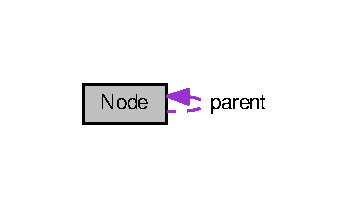
\includegraphics[width=169pt]{structNode__coll__graph}
\end{center}
\end{figure}
\subsection*{Public Attributes}
\begin{DoxyCompactItemize}
\item 
vector$<$ \hyperlink{structNode}{Node} $\ast$ $>$ \hyperlink{structNode_a4403c570a373595bc3f82a8ca0bd2e61}{children}
\item 
\hyperlink{structNode}{Node} $\ast$ \hyperlink{structNode_ad8184598cdea70e4bbdfd76f2b0f9e85}{parent}
\item 
Vector2f \hyperlink{structNode_a4894d1352134bef767e5c1aba7aa3207}{position}
\item 
float \hyperlink{structNode_a7515a1624b4a54ed344792f3458c167d}{orientation}
\item 
double \hyperlink{structNode_a6e7b74adca863064ca0d1684873f33e0}{cost}
\end{DoxyCompactItemize}


\subsection{Detailed Description}
R\+R\+T$\ast$ \hyperlink{structNode}{Node} strut. 

\subsection{Member Data Documentation}
\index{Node@{Node}!children@{children}}
\index{children@{children}!Node@{Node}}
\subsubsection[{\texorpdfstring{children}{children}}]{\setlength{\rightskip}{0pt plus 5cm}vector$<${\bf Node} $\ast$$>$ Node\+::children}\hypertarget{structNode_a4403c570a373595bc3f82a8ca0bd2e61}{}\label{structNode_a4403c570a373595bc3f82a8ca0bd2e61}
\index{Node@{Node}!cost@{cost}}
\index{cost@{cost}!Node@{Node}}
\subsubsection[{\texorpdfstring{cost}{cost}}]{\setlength{\rightskip}{0pt plus 5cm}double Node\+::cost}\hypertarget{structNode_a6e7b74adca863064ca0d1684873f33e0}{}\label{structNode_a6e7b74adca863064ca0d1684873f33e0}
\index{Node@{Node}!orientation@{orientation}}
\index{orientation@{orientation}!Node@{Node}}
\subsubsection[{\texorpdfstring{orientation}{orientation}}]{\setlength{\rightskip}{0pt plus 5cm}float Node\+::orientation}\hypertarget{structNode_a7515a1624b4a54ed344792f3458c167d}{}\label{structNode_a7515a1624b4a54ed344792f3458c167d}
\index{Node@{Node}!parent@{parent}}
\index{parent@{parent}!Node@{Node}}
\subsubsection[{\texorpdfstring{parent}{parent}}]{\setlength{\rightskip}{0pt plus 5cm}{\bf Node}$\ast$ Node\+::parent}\hypertarget{structNode_ad8184598cdea70e4bbdfd76f2b0f9e85}{}\label{structNode_ad8184598cdea70e4bbdfd76f2b0f9e85}
\index{Node@{Node}!position@{position}}
\index{position@{position}!Node@{Node}}
\subsubsection[{\texorpdfstring{position}{position}}]{\setlength{\rightskip}{0pt plus 5cm}Vector2f Node\+::position}\hypertarget{structNode_a4894d1352134bef767e5c1aba7aa3207}{}\label{structNode_a4894d1352134bef767e5c1aba7aa3207}


The documentation for this struct was generated from the following file\+:\begin{DoxyCompactItemize}
\item 
src/\+R\+R\+T\+Star/\hyperlink{rrtstar_8h}{rrtstar.\+h}\end{DoxyCompactItemize}

\hypertarget{structPath}{}\section{Path Struct Reference}
\label{structPath}\index{Path@{Path}}


A sequence of sampled robot configurations composing a (discretization of the) path.  




{\ttfamily \#include $<$utils.\+hpp$>$}

\subsection*{Public Member Functions}
\begin{DoxyCompactItemize}
\item 
\hyperlink{structPath_ad51cd6da6d625dccc562c98498d4675a}{Path} (std\+::vector$<$ \hyperlink{structPose}{Pose} $>$ const \&\hyperlink{structPath_a9847c298e904e1230b5706d22ed56c17}{points})
\item 
\hyperlink{structPath_af26cfab021ddf49af73da3b2beca85ac}{Path} ()
\item 
bool \hyperlink{structPath_aef5e0bd3594115a90bdbb9d8a0fb1cc5}{empty} ()
\item 
size\+\_\+t \hyperlink{structPath_ad6d1a267d775b7b9dcc5b6bfe1f8dd5a}{size} ()
\item 
void \hyperlink{structPath_a3e5e0ecbac2e7f869690ce9067815f5a}{set\+Points} (const std\+::vector$<$ \hyperlink{structPose}{Pose} $>$ \&\hyperlink{structPath_a9847c298e904e1230b5706d22ed56c17}{points})
\end{DoxyCompactItemize}
\subsection*{Public Attributes}
\begin{DoxyCompactItemize}
\item 
std\+::vector$<$ \hyperlink{structPose}{Pose} $>$ \hyperlink{structPath_a9847c298e904e1230b5706d22ed56c17}{points}
\end{DoxyCompactItemize}


\subsection{Detailed Description}
A sequence of sampled robot configurations composing a (discretization of the) path. 

\subsection{Constructor \& Destructor Documentation}
\index{Path@{Path}!Path@{Path}}
\index{Path@{Path}!Path@{Path}}
\subsubsection[{\texorpdfstring{Path(std\+::vector$<$ Pose $>$ const \&points)}{Path(std::vector< Pose > const &points)}}]{\setlength{\rightskip}{0pt plus 5cm}Path\+::\+Path (
\begin{DoxyParamCaption}
\item[{std\+::vector$<$ {\bf Pose} $>$ const \&}]{points}
\end{DoxyParamCaption}
)\hspace{0.3cm}{\ttfamily [inline]}}\hypertarget{structPath_ad51cd6da6d625dccc562c98498d4675a}{}\label{structPath_ad51cd6da6d625dccc562c98498d4675a}
\index{Path@{Path}!Path@{Path}}
\index{Path@{Path}!Path@{Path}}
\subsubsection[{\texorpdfstring{Path()}{Path()}}]{\setlength{\rightskip}{0pt plus 5cm}Path\+::\+Path (
\begin{DoxyParamCaption}
{}
\end{DoxyParamCaption}
)\hspace{0.3cm}{\ttfamily [inline]}}\hypertarget{structPath_af26cfab021ddf49af73da3b2beca85ac}{}\label{structPath_af26cfab021ddf49af73da3b2beca85ac}


\subsection{Member Function Documentation}
\index{Path@{Path}!empty@{empty}}
\index{empty@{empty}!Path@{Path}}
\subsubsection[{\texorpdfstring{empty()}{empty()}}]{\setlength{\rightskip}{0pt plus 5cm}bool Path\+::empty (
\begin{DoxyParamCaption}
{}
\end{DoxyParamCaption}
)\hspace{0.3cm}{\ttfamily [inline]}}\hypertarget{structPath_aef5e0bd3594115a90bdbb9d8a0fb1cc5}{}\label{structPath_aef5e0bd3594115a90bdbb9d8a0fb1cc5}
\index{Path@{Path}!set\+Points@{set\+Points}}
\index{set\+Points@{set\+Points}!Path@{Path}}
\subsubsection[{\texorpdfstring{set\+Points(const std\+::vector$<$ Pose $>$ \&points)}{setPoints(const std::vector< Pose > &points)}}]{\setlength{\rightskip}{0pt plus 5cm}void Path\+::set\+Points (
\begin{DoxyParamCaption}
\item[{const std\+::vector$<$ {\bf Pose} $>$ \&}]{points}
\end{DoxyParamCaption}
)\hspace{0.3cm}{\ttfamily [inline]}}\hypertarget{structPath_a3e5e0ecbac2e7f869690ce9067815f5a}{}\label{structPath_a3e5e0ecbac2e7f869690ce9067815f5a}
\index{Path@{Path}!size@{size}}
\index{size@{size}!Path@{Path}}
\subsubsection[{\texorpdfstring{size()}{size()}}]{\setlength{\rightskip}{0pt plus 5cm}size\+\_\+t Path\+::size (
\begin{DoxyParamCaption}
{}
\end{DoxyParamCaption}
)\hspace{0.3cm}{\ttfamily [inline]}}\hypertarget{structPath_ad6d1a267d775b7b9dcc5b6bfe1f8dd5a}{}\label{structPath_ad6d1a267d775b7b9dcc5b6bfe1f8dd5a}


\subsection{Member Data Documentation}
\index{Path@{Path}!points@{points}}
\index{points@{points}!Path@{Path}}
\subsubsection[{\texorpdfstring{points}{points}}]{\setlength{\rightskip}{0pt plus 5cm}std\+::vector$<${\bf Pose}$>$ Path\+::points}\hypertarget{structPath_a9847c298e904e1230b5706d22ed56c17}{}\label{structPath_a9847c298e904e1230b5706d22ed56c17}


The documentation for this struct was generated from the following file\+:\begin{DoxyCompactItemize}
\item 
/home/aravind/\+Desktop/\+Trento\+\_\+\+Exit/\+R\+P\+A/\+Workspace/simulator/src/9\+\_\+project\+\_\+interface/include/\hyperlink{utils_8hpp}{utils.\+hpp}\end{DoxyCompactItemize}

\hypertarget{structPoint}{}\section{Point Struct Reference}
\label{structPoint}\index{Point@{Point}}


\hyperlink{structPoint}{Point} in given space.  




{\ttfamily \#include $<$utils.\+hpp$>$}

\subsection*{Public Member Functions}
\begin{DoxyCompactItemize}
\item 
\hyperlink{structPoint_a30bc8409287de4f43e160664be834636}{Point} (float \hyperlink{structPoint_a05dfe2dfbde813ad234b514f30e662f1}{x}, float \hyperlink{structPoint_a6101960c8d2d4e8ea1d32c9234bbeb8d}{y})
\item 
\hyperlink{structPoint_ad92f2337b839a94ce97dcdb439b4325a}{Point} ()
\end{DoxyCompactItemize}
\subsection*{Public Attributes}
\begin{DoxyCompactItemize}
\item 
float \hyperlink{structPoint_a05dfe2dfbde813ad234b514f30e662f1}{x}
\item 
float \hyperlink{structPoint_a6101960c8d2d4e8ea1d32c9234bbeb8d}{y}
\end{DoxyCompactItemize}


\subsection{Detailed Description}
\hyperlink{structPoint}{Point} in given space. 

\subsection{Constructor \& Destructor Documentation}
\index{Point@{Point}!Point@{Point}}
\index{Point@{Point}!Point@{Point}}
\subsubsection[{\texorpdfstring{Point(float x, float y)}{Point(float x, float y)}}]{\setlength{\rightskip}{0pt plus 5cm}Point\+::\+Point (
\begin{DoxyParamCaption}
\item[{float}]{x, }
\item[{float}]{y}
\end{DoxyParamCaption}
)\hspace{0.3cm}{\ttfamily [inline]}}\hypertarget{structPoint_a30bc8409287de4f43e160664be834636}{}\label{structPoint_a30bc8409287de4f43e160664be834636}
\index{Point@{Point}!Point@{Point}}
\index{Point@{Point}!Point@{Point}}
\subsubsection[{\texorpdfstring{Point()}{Point()}}]{\setlength{\rightskip}{0pt plus 5cm}Point\+::\+Point (
\begin{DoxyParamCaption}
{}
\end{DoxyParamCaption}
)\hspace{0.3cm}{\ttfamily [inline]}}\hypertarget{structPoint_ad92f2337b839a94ce97dcdb439b4325a}{}\label{structPoint_ad92f2337b839a94ce97dcdb439b4325a}


\subsection{Member Data Documentation}
\index{Point@{Point}!x@{x}}
\index{x@{x}!Point@{Point}}
\subsubsection[{\texorpdfstring{x}{x}}]{\setlength{\rightskip}{0pt plus 5cm}float Point\+::x}\hypertarget{structPoint_a05dfe2dfbde813ad234b514f30e662f1}{}\label{structPoint_a05dfe2dfbde813ad234b514f30e662f1}
\index{Point@{Point}!y@{y}}
\index{y@{y}!Point@{Point}}
\subsubsection[{\texorpdfstring{y}{y}}]{\setlength{\rightskip}{0pt plus 5cm}float Point\+::y}\hypertarget{structPoint_a6101960c8d2d4e8ea1d32c9234bbeb8d}{}\label{structPoint_a6101960c8d2d4e8ea1d32c9234bbeb8d}


The documentation for this struct was generated from the following file\+:\begin{DoxyCompactItemize}
\item 
/home/aravind/\+Desktop/\+Trento\+\_\+\+Exit/\+R\+P\+A/\+Workspace/simulator/src/9\+\_\+project\+\_\+interface/include/\hyperlink{utils_8hpp}{utils.\+hpp}\end{DoxyCompactItemize}

\hypertarget{structPose}{}\section{Pose Struct Reference}
\label{structPose}\index{Pose@{Pose}}


A configuration of the robot along the path, represented by x, y, orientation and curvature.  




{\ttfamily \#include $<$utils.\+hpp$>$}

\subsection*{Public Member Functions}
\begin{DoxyCompactItemize}
\item 
\hyperlink{structPose_a80c8e028bf0a6d815db4bbd599877f22}{Pose} (float \hyperlink{structPose_a7cafd5a1122c053e9c1ddec351dbb8f3}{s}, float \hyperlink{structPose_a2f30fe76d6747d973daff013207ca0e8}{x}, float \hyperlink{structPose_a60610dad0457edf9e1c57a787b68b632}{y}, float \hyperlink{structPose_a2e2edc8448a8f6f4a21cbd7eca63c2ff}{theta}, float \hyperlink{structPose_a4f409e1fe4ae5626042bc2942df9367a}{kappa})
\item 
\hyperlink{structPose_a8a4171c8a6b09e37fb011997da9ea2ad}{Pose} ()
\item 
float \hyperlink{structPose_a2032faa5456e2d667bac87f7f8921020}{distance} (float \+\_\+x, float \+\_\+y)
\end{DoxyCompactItemize}
\subsection*{Public Attributes}
\begin{DoxyCompactItemize}
\item 
float \hyperlink{structPose_a7cafd5a1122c053e9c1ddec351dbb8f3}{s}
\item 
float \hyperlink{structPose_a2f30fe76d6747d973daff013207ca0e8}{x}
\item 
float \hyperlink{structPose_a60610dad0457edf9e1c57a787b68b632}{y}
\item 
float \hyperlink{structPose_a2e2edc8448a8f6f4a21cbd7eca63c2ff}{theta}
\item 
float \hyperlink{structPose_a4f409e1fe4ae5626042bc2942df9367a}{kappa}
\end{DoxyCompactItemize}


\subsection{Detailed Description}
A configuration of the robot along the path, represented by x, y, orientation and curvature. 

\subsection{Constructor \& Destructor Documentation}
\index{Pose@{Pose}!Pose@{Pose}}
\index{Pose@{Pose}!Pose@{Pose}}
\subsubsection[{\texorpdfstring{Pose(float s, float x, float y, float theta, float kappa)}{Pose(float s, float x, float y, float theta, float kappa)}}]{\setlength{\rightskip}{0pt plus 5cm}Pose\+::\+Pose (
\begin{DoxyParamCaption}
\item[{float}]{s, }
\item[{float}]{x, }
\item[{float}]{y, }
\item[{float}]{theta, }
\item[{float}]{kappa}
\end{DoxyParamCaption}
)\hspace{0.3cm}{\ttfamily [inline]}}\hypertarget{structPose_a80c8e028bf0a6d815db4bbd599877f22}{}\label{structPose_a80c8e028bf0a6d815db4bbd599877f22}
\index{Pose@{Pose}!Pose@{Pose}}
\index{Pose@{Pose}!Pose@{Pose}}
\subsubsection[{\texorpdfstring{Pose()}{Pose()}}]{\setlength{\rightskip}{0pt plus 5cm}Pose\+::\+Pose (
\begin{DoxyParamCaption}
{}
\end{DoxyParamCaption}
)\hspace{0.3cm}{\ttfamily [inline]}}\hypertarget{structPose_a8a4171c8a6b09e37fb011997da9ea2ad}{}\label{structPose_a8a4171c8a6b09e37fb011997da9ea2ad}


\subsection{Member Function Documentation}
\index{Pose@{Pose}!distance@{distance}}
\index{distance@{distance}!Pose@{Pose}}
\subsubsection[{\texorpdfstring{distance(float \+\_\+x, float \+\_\+y)}{distance(float _x, float _y)}}]{\setlength{\rightskip}{0pt plus 5cm}float Pose\+::distance (
\begin{DoxyParamCaption}
\item[{float}]{\+\_\+x, }
\item[{float}]{\+\_\+y}
\end{DoxyParamCaption}
)\hspace{0.3cm}{\ttfamily [inline]}}\hypertarget{structPose_a2032faa5456e2d667bac87f7f8921020}{}\label{structPose_a2032faa5456e2d667bac87f7f8921020}


\subsection{Member Data Documentation}
\index{Pose@{Pose}!kappa@{kappa}}
\index{kappa@{kappa}!Pose@{Pose}}
\subsubsection[{\texorpdfstring{kappa}{kappa}}]{\setlength{\rightskip}{0pt plus 5cm}float Pose\+::kappa}\hypertarget{structPose_a4f409e1fe4ae5626042bc2942df9367a}{}\label{structPose_a4f409e1fe4ae5626042bc2942df9367a}
\index{Pose@{Pose}!s@{s}}
\index{s@{s}!Pose@{Pose}}
\subsubsection[{\texorpdfstring{s}{s}}]{\setlength{\rightskip}{0pt plus 5cm}float Pose\+::s}\hypertarget{structPose_a7cafd5a1122c053e9c1ddec351dbb8f3}{}\label{structPose_a7cafd5a1122c053e9c1ddec351dbb8f3}
\index{Pose@{Pose}!theta@{theta}}
\index{theta@{theta}!Pose@{Pose}}
\subsubsection[{\texorpdfstring{theta}{theta}}]{\setlength{\rightskip}{0pt plus 5cm}float Pose\+::theta}\hypertarget{structPose_a2e2edc8448a8f6f4a21cbd7eca63c2ff}{}\label{structPose_a2e2edc8448a8f6f4a21cbd7eca63c2ff}
\index{Pose@{Pose}!x@{x}}
\index{x@{x}!Pose@{Pose}}
\subsubsection[{\texorpdfstring{x}{x}}]{\setlength{\rightskip}{0pt plus 5cm}float Pose\+::x}\hypertarget{structPose_a2f30fe76d6747d973daff013207ca0e8}{}\label{structPose_a2f30fe76d6747d973daff013207ca0e8}
\index{Pose@{Pose}!y@{y}}
\index{y@{y}!Pose@{Pose}}
\subsubsection[{\texorpdfstring{y}{y}}]{\setlength{\rightskip}{0pt plus 5cm}float Pose\+::y}\hypertarget{structPose_a60610dad0457edf9e1c57a787b68b632}{}\label{structPose_a60610dad0457edf9e1c57a787b68b632}


The documentation for this struct was generated from the following file\+:\begin{DoxyCompactItemize}
\item 
/home/aravind/\+Desktop/\+Trento\+\_\+\+Exit/\+R\+P\+A/\+Workspace/simulator/src/9\+\_\+project\+\_\+interface/include/\hyperlink{utils_8hpp}{utils.\+hpp}\end{DoxyCompactItemize}

\hypertarget{classRRTObstacles}{}\section{R\+R\+T\+Obstacles Class Reference}
\label{classRRTObstacles}\index{R\+R\+T\+Obstacles@{R\+R\+T\+Obstacles}}


Obstacles class for R\+R\+T$\ast$ Star Implementation.  




{\ttfamily \#include $<$obstacles.\+h$>$}

\subsection*{Public Member Functions}
\begin{DoxyCompactItemize}
\item 
\hyperlink{classRRTObstacles_a2a8b080aee81476a84987f9cc3aa6186}{R\+R\+T\+Obstacles} ()
\item 
void \hyperlink{classRRTObstacles_a0359d5f53c91410a35eb1bbb8920f8dc}{add\+Obstacle} (double radius, Vector2f second\+Point)
\begin{DoxyCompactList}\small\item\em Obstacles are stored as circles. Circles is denoted by center point and radius. \end{DoxyCompactList}\item 
bool \hyperlink{classRRTObstacles_a1bf5b6afa6aa7704584febd7b2d1550a}{is\+Segment\+In\+Obstacle} (Vector2f \&p1, Vector2f \&p2)
\begin{DoxyCompactList}\small\item\em Check if a line segment intersects a rectangle. \end{DoxyCompactList}\end{DoxyCompactItemize}
\subsection*{Public Attributes}
\begin{DoxyCompactItemize}
\item 
vector$<$ pair$<$ double, Vector2f $>$ $>$ \hyperlink{classRRTObstacles_a0bbd43d5b8ddeb2f293f689d09c26947}{obstacles}
\end{DoxyCompactItemize}


\subsection{Detailed Description}
Obstacles class for R\+R\+T$\ast$ Star Implementation. 

\subsection{Constructor \& Destructor Documentation}
\index{R\+R\+T\+Obstacles@{R\+R\+T\+Obstacles}!R\+R\+T\+Obstacles@{R\+R\+T\+Obstacles}}
\index{R\+R\+T\+Obstacles@{R\+R\+T\+Obstacles}!R\+R\+T\+Obstacles@{R\+R\+T\+Obstacles}}
\subsubsection[{\texorpdfstring{R\+R\+T\+Obstacles()}{RRTObstacles()}}]{\setlength{\rightskip}{0pt plus 5cm}R\+R\+T\+Obstacles\+::\+R\+R\+T\+Obstacles (
\begin{DoxyParamCaption}
{}
\end{DoxyParamCaption}
)}\hypertarget{classRRTObstacles_a2a8b080aee81476a84987f9cc3aa6186}{}\label{classRRTObstacles_a2a8b080aee81476a84987f9cc3aa6186}


\subsection{Member Function Documentation}
\index{R\+R\+T\+Obstacles@{R\+R\+T\+Obstacles}!add\+Obstacle@{add\+Obstacle}}
\index{add\+Obstacle@{add\+Obstacle}!R\+R\+T\+Obstacles@{R\+R\+T\+Obstacles}}
\subsubsection[{\texorpdfstring{add\+Obstacle(double radius, Vector2f second\+Point)}{addObstacle(double radius, Vector2f secondPoint)}}]{\setlength{\rightskip}{0pt plus 5cm}void R\+R\+T\+Obstacles\+::add\+Obstacle (
\begin{DoxyParamCaption}
\item[{double}]{radius, }
\item[{Vector2f}]{center\+Point}
\end{DoxyParamCaption}
)}\hypertarget{classRRTObstacles_a0359d5f53c91410a35eb1bbb8920f8dc}{}\label{classRRTObstacles_a0359d5f53c91410a35eb1bbb8920f8dc}


Obstacles are stored as circles. Circles is denoted by center point and radius. 


\begin{DoxyParams}{Parameters}
{\em radius} & \\
\hline
{\em center\+Point} & \\
\hline
\end{DoxyParams}
\index{R\+R\+T\+Obstacles@{R\+R\+T\+Obstacles}!is\+Segment\+In\+Obstacle@{is\+Segment\+In\+Obstacle}}
\index{is\+Segment\+In\+Obstacle@{is\+Segment\+In\+Obstacle}!R\+R\+T\+Obstacles@{R\+R\+T\+Obstacles}}
\subsubsection[{\texorpdfstring{is\+Segment\+In\+Obstacle(\+Vector2f \&p1, Vector2f \&p2)}{isSegmentInObstacle(Vector2f &p1, Vector2f &p2)}}]{\setlength{\rightskip}{0pt plus 5cm}bool R\+R\+T\+Obstacles\+::is\+Segment\+In\+Obstacle (
\begin{DoxyParamCaption}
\item[{Vector2f \&}]{p1, }
\item[{Vector2f \&}]{p2}
\end{DoxyParamCaption}
)}\hypertarget{classRRTObstacles_a1bf5b6afa6aa7704584febd7b2d1550a}{}\label{classRRTObstacles_a1bf5b6afa6aa7704584febd7b2d1550a}


Check if a line segment intersects a rectangle. 


\begin{DoxyParams}{Parameters}
{\em p1} & \\
\hline
{\em p2} & \\
\hline
\end{DoxyParams}
\begin{DoxyReturn}{Returns}

\end{DoxyReturn}


\subsection{Member Data Documentation}
\index{R\+R\+T\+Obstacles@{R\+R\+T\+Obstacles}!obstacles@{obstacles}}
\index{obstacles@{obstacles}!R\+R\+T\+Obstacles@{R\+R\+T\+Obstacles}}
\subsubsection[{\texorpdfstring{obstacles}{obstacles}}]{\setlength{\rightskip}{0pt plus 5cm}vector$<$pair$<$double, Vector2f$>$ $>$ R\+R\+T\+Obstacles\+::obstacles}\hypertarget{classRRTObstacles_a0bbd43d5b8ddeb2f293f689d09c26947}{}\label{classRRTObstacles_a0bbd43d5b8ddeb2f293f689d09c26947}


The documentation for this class was generated from the following files\+:\begin{DoxyCompactItemize}
\item 
src/\+R\+R\+T\+Star/\hyperlink{obstacles_8h}{obstacles.\+h}\item 
src/\+R\+R\+T\+Star/\hyperlink{obstacles_8cpp}{obstacles.\+cpp}\end{DoxyCompactItemize}

\hypertarget{classRRTSTAR}{}\section{R\+R\+T\+S\+T\+AR Class Reference}
\label{classRRTSTAR}\index{R\+R\+T\+S\+T\+AR@{R\+R\+T\+S\+T\+AR}}


R\+R\+T\+Star Class.  




{\ttfamily \#include $<$rrtstar.\+h$>$}



Collaboration diagram for R\+R\+T\+S\+T\+AR\+:\nopagebreak
\begin{figure}[H]
\begin{center}
\leavevmode
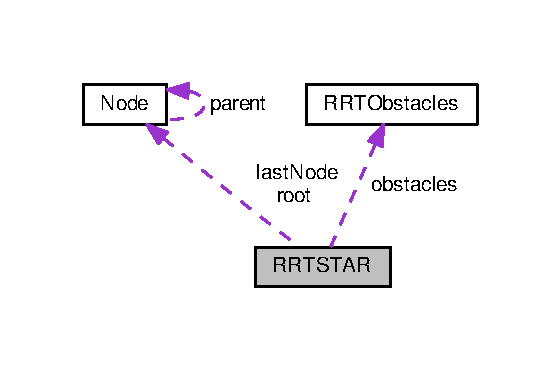
\includegraphics[width=269pt]{classRRTSTAR__coll__graph}
\end{center}
\end{figure}
\subsection*{Public Member Functions}
\begin{DoxyCompactItemize}
\item 
\hyperlink{classRRTSTAR_ad9c4671d299e90158b61621959ac646f}{R\+R\+T\+S\+T\+AR} ()
\begin{DoxyCompactList}\small\item\em Constructor. \end{DoxyCompactList}\item 
void \hyperlink{classRRTSTAR_aba683c9684e61576e5833b2293a0c589}{initialize} ()
\begin{DoxyCompactList}\small\item\em Initialize root node of \hyperlink{classRRTSTAR}{R\+R\+T\+S\+T\+AR}. \end{DoxyCompactList}\item 
\hyperlink{structNode}{Node} $\ast$ \hyperlink{classRRTSTAR_a52b217b8070afabc733451923e482c55}{get\+Random\+Node} ()
\begin{DoxyCompactList}\small\item\em Generate a random node in the field. \end{DoxyCompactList}\item 
\hyperlink{structNode}{Node} $\ast$ \hyperlink{classRRTSTAR_a17b8392462e01ed383e7ba01d9ff7917}{nearest} (Vector2f point)
\begin{DoxyCompactList}\small\item\em Get nearest node from a given configuration/position. \end{DoxyCompactList}\item 
void \hyperlink{classRRTSTAR_a206d008a7e35e8da67ba45e69dda614e}{near} (Vector2f point, float radius, vector$<$ \hyperlink{structNode}{Node} $\ast$ $>$ \&out\+\_\+nodes)
\begin{DoxyCompactList}\small\item\em Get neighborhood nodes of a given configuration/position. \end{DoxyCompactList}\item 
double \hyperlink{classRRTSTAR_a6b25100958bc2983c8e884e06a1781fd}{distance} (Vector2f \&p, Vector2f \&q)
\begin{DoxyCompactList}\small\item\em Helper method to find distance between two positions. \end{DoxyCompactList}\item 
double \hyperlink{classRRTSTAR_aff52d6be37b207ad4bef71430736fa06}{Cost} (\hyperlink{structNode}{Node} $\ast$q)
\begin{DoxyCompactList}\small\item\em Return trajectory cost. \end{DoxyCompactList}\item 
double \hyperlink{classRRTSTAR_aec4f110bd8cf010d2c86f235306996e7}{Path\+Cost} (\hyperlink{structNode}{Node} $\ast$q\+From, \hyperlink{structNode}{Node} $\ast$q\+To)
\begin{DoxyCompactList}\small\item\em Compute path cost. \end{DoxyCompactList}\item 
Vector3f \hyperlink{classRRTSTAR_a7519aad88048588ebc11bfb04a1c1b4a}{new\+Config} (\hyperlink{structNode}{Node} $\ast$q, \hyperlink{structNode}{Node} $\ast$q\+Nearest)
\begin{DoxyCompactList}\small\item\em Find a configuration at a distance step\+\_\+size from nearest node to random node. \end{DoxyCompactList}\item 
void \hyperlink{classRRTSTAR_a857eb7050319c4f0950724ae150e597b}{add} (\hyperlink{structNode}{Node} $\ast$q\+Nearest, \hyperlink{structNode}{Node} $\ast$q\+New)
\begin{DoxyCompactList}\small\item\em Add a node to the tree. \end{DoxyCompactList}\item 
bool \hyperlink{classRRTSTAR_a999e6db04aff2b7b5d3c66e50b3057b8}{reached} ()
\begin{DoxyCompactList}\small\item\em Check if the last node is close to the end position. \end{DoxyCompactList}\item 
void \hyperlink{classRRTSTAR_add28ae0f961e4fe1d35ebdfb95bf7365}{set\+Step\+Size} (double step)
\item 
void \hyperlink{classRRTSTAR_a3b0e2de2074b31567b8eb65a082de463}{set\+Max\+Iterations} (int iter)
\item 
void \hyperlink{classRRTSTAR_a8aa26cd3eab9eed58746ceaa5a7b68f0}{delete\+Nodes} (\hyperlink{structNode}{Node} $\ast$\hyperlink{classRRTSTAR_a93a4dad750b6a408269ca45a4b618d4e}{root})
\begin{DoxyCompactList}\small\item\em Delete all nodes using D\+FS technique. \end{DoxyCompactList}\item 
void \hyperlink{classRRTSTAR_a79020afd3dae6e89caca9704810db7fd}{set\+Start\+Pose} (double x, double y, double theta)
\begin{DoxyCompactList}\small\item\em Set the Start position of robot. \end{DoxyCompactList}\item 
void \hyperlink{classRRTSTAR_af4f27caedca02db30d70e07ec5a35a34}{set\+Goal\+Pose} (double x, double y)
\begin{DoxyCompactList}\small\item\em Set the Destination position. \end{DoxyCompactList}\item 
void \hyperlink{classRRTSTAR_ac9e0362f930ea0794eb94f30a34b9147}{set\+World\+Info} (double width, double height)
\begin{DoxyCompactList}\small\item\em Set the World information. \end{DoxyCompactList}\item 
void \hyperlink{classRRTSTAR_a85a72ab7c47e0fcf1d464a75af1ed309}{set\+\_\+max\+\_\+iter} (int x)
\item 
void \hyperlink{classRRTSTAR_ad0f94ca8a2bfddd676adca784bf69c07}{set\+\_\+step\+\_\+size} (double x)
\item 
void \hyperlink{classRRTSTAR_a92d71705680b9cdfe3b42982168e320a}{set\+\_\+bot\+\_\+radius} (double x)
\item 
void \hyperlink{classRRTSTAR_a4e57768e18f20604fffd50cd5a60af8d}{set\+\_\+goal\+Bias} (double x)
\item 
void \hyperlink{classRRTSTAR_a1a65e27cb565f2adf789dd582252a8a6}{set\+\_\+turn\+\_\+radius} (double x)
\item 
void \hyperlink{classRRTSTAR_a297bbde6f019ac7ae876ce9c2608cd9b}{set\+\_\+rrt\+\_\+star\+\_\+neighbour\+\_\+factor} (double x)
\item 
void \hyperlink{classRRTSTAR_a6b06cbc77a08446e0c97b8da9786afd6}{set\+\_\+bot\+\_\+follow\+\_\+dubin} (bool x)
\end{DoxyCompactItemize}
\subsection*{Public Attributes}
\begin{DoxyCompactItemize}
\item 
\hyperlink{classRRTObstacles}{R\+R\+T\+Obstacles} $\ast$ \hyperlink{classRRTSTAR_a3d9f67d4f4efa9681148b683e7b2455c}{obstacles}
\item 
vector$<$ \hyperlink{structNode}{Node} $\ast$ $>$ \hyperlink{classRRTSTAR_aef5c314d28c8ec948f07efa5f4cabefe}{nodes}
\item 
vector$<$ \hyperlink{structNode}{Node} $\ast$ $>$ \hyperlink{classRRTSTAR_a3c4afcfe867e23c36e268aedd488e062}{path}
\item 
\hyperlink{structNode}{Node} $\ast$ \hyperlink{classRRTSTAR_a93a4dad750b6a408269ca45a4b618d4e}{root}
\item 
\hyperlink{structNode}{Node} $\ast$ \hyperlink{classRRTSTAR_a46e3d08a8bd512c4f5747cdfbea41228}{last\+Node}
\item 
Vector2f \hyperlink{classRRTSTAR_ab3a0269ff354a27408ae48011a0e29f8}{start\+Pos}
\item 
Vector2f \hyperlink{classRRTSTAR_a220f337b1e11e8308b1bb590e0ff926a}{end\+Pos}
\item 
double \hyperlink{classRRTSTAR_a571433cf52df263c3e866c317e0ac4e3}{start\+\_\+orient}
\item 
int \hyperlink{classRRTSTAR_a9831be75ba6cce1bddfba73c9639e8c4}{max\+\_\+iter}
\item 
double \hyperlink{classRRTSTAR_a6e49feee90b9dd0a780444ff07520512}{step\+\_\+size}
\item 
double \hyperlink{classRRTSTAR_adc9c88a24560ab3a537ea374672b0121}{world\+\_\+width}
\item 
double \hyperlink{classRRTSTAR_a03ea0b6f54575f892d24553db558ce11}{world\+\_\+height}
\item 
double \hyperlink{classRRTSTAR_ac630bd4c26bf038a9158f02e4af761b4}{bot\+\_\+radius}
\item 
double \hyperlink{classRRTSTAR_ab458943c70394087a8ddc5f8b2f0fc79}{goal\+Bias}
\item 
double \hyperlink{classRRTSTAR_a72f670ad016b3e6bbf4a429873362c11}{turn\+\_\+radius}
\item 
bool \hyperlink{classRRTSTAR_a7325b9cbe347fded3d2541e017207c9e}{bot\+\_\+follow\+\_\+dubin}
\item 
double \hyperlink{classRRTSTAR_acb06c8a7193ad7776cf155a10142c5c3}{rrt\+\_\+star\+\_\+neighbour\+\_\+factor}
\end{DoxyCompactItemize}


\subsection{Detailed Description}
R\+R\+T\+Star Class. 

\subsection{Constructor \& Destructor Documentation}
\index{R\+R\+T\+S\+T\+AR@{R\+R\+T\+S\+T\+AR}!R\+R\+T\+S\+T\+AR@{R\+R\+T\+S\+T\+AR}}
\index{R\+R\+T\+S\+T\+AR@{R\+R\+T\+S\+T\+AR}!R\+R\+T\+S\+T\+AR@{R\+R\+T\+S\+T\+AR}}
\subsubsection[{\texorpdfstring{R\+R\+T\+S\+T\+A\+R()}{RRTSTAR()}}]{\setlength{\rightskip}{0pt plus 5cm}R\+R\+T\+S\+T\+A\+R\+::\+R\+R\+T\+S\+T\+AR (
\begin{DoxyParamCaption}
{}
\end{DoxyParamCaption}
)}\hypertarget{classRRTSTAR_ad9c4671d299e90158b61621959ac646f}{}\label{classRRTSTAR_ad9c4671d299e90158b61621959ac646f}


Constructor. 



\subsection{Member Function Documentation}
\index{R\+R\+T\+S\+T\+AR@{R\+R\+T\+S\+T\+AR}!add@{add}}
\index{add@{add}!R\+R\+T\+S\+T\+AR@{R\+R\+T\+S\+T\+AR}}
\subsubsection[{\texorpdfstring{add(\+Node $\ast$q\+Nearest, Node $\ast$q\+New)}{add(Node *qNearest, Node *qNew)}}]{\setlength{\rightskip}{0pt plus 5cm}void R\+R\+T\+S\+T\+A\+R\+::add (
\begin{DoxyParamCaption}
\item[{{\bf Node} $\ast$}]{q\+Nearest, }
\item[{{\bf Node} $\ast$}]{q\+New}
\end{DoxyParamCaption}
)}\hypertarget{classRRTSTAR_a857eb7050319c4f0950724ae150e597b}{}\label{classRRTSTAR_a857eb7050319c4f0950724ae150e597b}


Add a node to the tree. 


\begin{DoxyParams}{Parameters}
{\em q\+Nearest} & \\
\hline
{\em q\+New} & \\
\hline
\end{DoxyParams}
\index{R\+R\+T\+S\+T\+AR@{R\+R\+T\+S\+T\+AR}!Cost@{Cost}}
\index{Cost@{Cost}!R\+R\+T\+S\+T\+AR@{R\+R\+T\+S\+T\+AR}}
\subsubsection[{\texorpdfstring{Cost(\+Node $\ast$q)}{Cost(Node *q)}}]{\setlength{\rightskip}{0pt plus 5cm}double R\+R\+T\+S\+T\+A\+R\+::\+Cost (
\begin{DoxyParamCaption}
\item[{{\bf Node} $\ast$}]{q}
\end{DoxyParamCaption}
)}\hypertarget{classRRTSTAR_aff52d6be37b207ad4bef71430736fa06}{}\label{classRRTSTAR_aff52d6be37b207ad4bef71430736fa06}


Return trajectory cost. 


\begin{DoxyParams}{Parameters}
{\em q} & cost of node be computed \\
\hline
\end{DoxyParams}
\begin{DoxyReturn}{Returns}
Cost of the node 
\end{DoxyReturn}
\index{R\+R\+T\+S\+T\+AR@{R\+R\+T\+S\+T\+AR}!delete\+Nodes@{delete\+Nodes}}
\index{delete\+Nodes@{delete\+Nodes}!R\+R\+T\+S\+T\+AR@{R\+R\+T\+S\+T\+AR}}
\subsubsection[{\texorpdfstring{delete\+Nodes(\+Node $\ast$root)}{deleteNodes(Node *root)}}]{\setlength{\rightskip}{0pt plus 5cm}void R\+R\+T\+S\+T\+A\+R\+::delete\+Nodes (
\begin{DoxyParamCaption}
\item[{{\bf Node} $\ast$}]{root}
\end{DoxyParamCaption}
)}\hypertarget{classRRTSTAR_a8aa26cd3eab9eed58746ceaa5a7b68f0}{}\label{classRRTSTAR_a8aa26cd3eab9eed58746ceaa5a7b68f0}


Delete all nodes using D\+FS technique. 


\begin{DoxyParams}{Parameters}
{\em root} & root node or the first node \\
\hline
\end{DoxyParams}
\index{R\+R\+T\+S\+T\+AR@{R\+R\+T\+S\+T\+AR}!distance@{distance}}
\index{distance@{distance}!R\+R\+T\+S\+T\+AR@{R\+R\+T\+S\+T\+AR}}
\subsubsection[{\texorpdfstring{distance(\+Vector2f \&p, Vector2f \&q)}{distance(Vector2f &p, Vector2f &q)}}]{\setlength{\rightskip}{0pt plus 5cm}double R\+R\+T\+S\+T\+A\+R\+::distance (
\begin{DoxyParamCaption}
\item[{Vector2f \&}]{p, }
\item[{Vector2f \&}]{q}
\end{DoxyParamCaption}
)}\hypertarget{classRRTSTAR_a6b25100958bc2983c8e884e06a1781fd}{}\label{classRRTSTAR_a6b25100958bc2983c8e884e06a1781fd}


Helper method to find distance between two positions. 


\begin{DoxyParams}{Parameters}
{\em p} & \hyperlink{structPoint}{Point} p \\
\hline
{\em q} & \hyperlink{structPoint}{Point} q \\
\hline
\end{DoxyParams}
\begin{DoxyReturn}{Returns}
Euclidean distance between \hyperlink{structPoint}{Point} P and Q 
\end{DoxyReturn}
\index{R\+R\+T\+S\+T\+AR@{R\+R\+T\+S\+T\+AR}!get\+Random\+Node@{get\+Random\+Node}}
\index{get\+Random\+Node@{get\+Random\+Node}!R\+R\+T\+S\+T\+AR@{R\+R\+T\+S\+T\+AR}}
\subsubsection[{\texorpdfstring{get\+Random\+Node()}{getRandomNode()}}]{\setlength{\rightskip}{0pt plus 5cm}{\bf Node} $\ast$ R\+R\+T\+S\+T\+A\+R\+::get\+Random\+Node (
\begin{DoxyParamCaption}
{}
\end{DoxyParamCaption}
)}\hypertarget{classRRTSTAR_a52b217b8070afabc733451923e482c55}{}\label{classRRTSTAR_a52b217b8070afabc733451923e482c55}


Generate a random node in the field. 

\begin{DoxyReturn}{Returns}
Random \hyperlink{structNode}{Node} 
\end{DoxyReturn}
\index{R\+R\+T\+S\+T\+AR@{R\+R\+T\+S\+T\+AR}!initialize@{initialize}}
\index{initialize@{initialize}!R\+R\+T\+S\+T\+AR@{R\+R\+T\+S\+T\+AR}}
\subsubsection[{\texorpdfstring{initialize()}{initialize()}}]{\setlength{\rightskip}{0pt plus 5cm}void R\+R\+T\+S\+T\+A\+R\+::initialize (
\begin{DoxyParamCaption}
{}
\end{DoxyParamCaption}
)}\hypertarget{classRRTSTAR_aba683c9684e61576e5833b2293a0c589}{}\label{classRRTSTAR_aba683c9684e61576e5833b2293a0c589}


Initialize root node of \hyperlink{classRRTSTAR}{R\+R\+T\+S\+T\+AR}. 

\index{R\+R\+T\+S\+T\+AR@{R\+R\+T\+S\+T\+AR}!near@{near}}
\index{near@{near}!R\+R\+T\+S\+T\+AR@{R\+R\+T\+S\+T\+AR}}
\subsubsection[{\texorpdfstring{near(\+Vector2f point, float radius, vector$<$ Node $\ast$ $>$ \&out\+\_\+nodes)}{near(Vector2f point, float radius, vector< Node * > &out_nodes)}}]{\setlength{\rightskip}{0pt plus 5cm}void R\+R\+T\+S\+T\+A\+R\+::near (
\begin{DoxyParamCaption}
\item[{Vector2f}]{point, }
\item[{float}]{radius, }
\item[{vector$<$ {\bf Node} $\ast$ $>$ \&}]{out\+\_\+nodes}
\end{DoxyParamCaption}
)}\hypertarget{classRRTSTAR_a206d008a7e35e8da67ba45e69dda614e}{}\label{classRRTSTAR_a206d008a7e35e8da67ba45e69dda614e}


Get neighborhood nodes of a given configuration/position. 


\begin{DoxyParams}{Parameters}
{\em point} & point in the world \\
\hline
{\em radius} & radius to check for neighbors \\
\hline
{\em out\+\_\+nodes} & list of nodes in that radius \\
\hline
\end{DoxyParams}
\index{R\+R\+T\+S\+T\+AR@{R\+R\+T\+S\+T\+AR}!nearest@{nearest}}
\index{nearest@{nearest}!R\+R\+T\+S\+T\+AR@{R\+R\+T\+S\+T\+AR}}
\subsubsection[{\texorpdfstring{nearest(\+Vector2f point)}{nearest(Vector2f point)}}]{\setlength{\rightskip}{0pt plus 5cm}{\bf Node} $\ast$ R\+R\+T\+S\+T\+A\+R\+::nearest (
\begin{DoxyParamCaption}
\item[{Vector2f}]{point}
\end{DoxyParamCaption}
)}\hypertarget{classRRTSTAR_a17b8392462e01ed383e7ba01d9ff7917}{}\label{classRRTSTAR_a17b8392462e01ed383e7ba01d9ff7917}


Get nearest node from a given configuration/position. 


\begin{DoxyParams}{Parameters}
{\em point} & given point in world \\
\hline
\end{DoxyParams}
\begin{DoxyReturn}{Returns}
Nearest \hyperlink{structNode}{Node} in the node list 
\end{DoxyReturn}
\index{R\+R\+T\+S\+T\+AR@{R\+R\+T\+S\+T\+AR}!new\+Config@{new\+Config}}
\index{new\+Config@{new\+Config}!R\+R\+T\+S\+T\+AR@{R\+R\+T\+S\+T\+AR}}
\subsubsection[{\texorpdfstring{new\+Config(\+Node $\ast$q, Node $\ast$q\+Nearest)}{newConfig(Node *q, Node *qNearest)}}]{\setlength{\rightskip}{0pt plus 5cm}Vector3f R\+R\+T\+S\+T\+A\+R\+::new\+Config (
\begin{DoxyParamCaption}
\item[{{\bf Node} $\ast$}]{q, }
\item[{{\bf Node} $\ast$}]{q\+Nearest}
\end{DoxyParamCaption}
)}\hypertarget{classRRTSTAR_a7519aad88048588ebc11bfb04a1c1b4a}{}\label{classRRTSTAR_a7519aad88048588ebc11bfb04a1c1b4a}


Find a configuration at a distance step\+\_\+size from nearest node to random node. 


\begin{DoxyParams}{Parameters}
{\em q} & given node \\
\hline
{\em q\+Nearest} & nearest node in list \\
\hline
\end{DoxyParams}
\begin{DoxyReturn}{Returns}
New config with (x,y,theta) 
\end{DoxyReturn}
\index{R\+R\+T\+S\+T\+AR@{R\+R\+T\+S\+T\+AR}!Path\+Cost@{Path\+Cost}}
\index{Path\+Cost@{Path\+Cost}!R\+R\+T\+S\+T\+AR@{R\+R\+T\+S\+T\+AR}}
\subsubsection[{\texorpdfstring{Path\+Cost(\+Node $\ast$q\+From, Node $\ast$q\+To)}{PathCost(Node *qFrom, Node *qTo)}}]{\setlength{\rightskip}{0pt plus 5cm}double R\+R\+T\+S\+T\+A\+R\+::\+Path\+Cost (
\begin{DoxyParamCaption}
\item[{{\bf Node} $\ast$}]{q\+From, }
\item[{{\bf Node} $\ast$}]{q\+To}
\end{DoxyParamCaption}
)}\hypertarget{classRRTSTAR_aec4f110bd8cf010d2c86f235306996e7}{}\label{classRRTSTAR_aec4f110bd8cf010d2c86f235306996e7}


Compute path cost. 


\begin{DoxyParams}{Parameters}
{\em q\+From} & from node \\
\hline
{\em q\+To} & to node \\
\hline
\end{DoxyParams}
\begin{DoxyReturn}{Returns}
The path cost from \hyperlink{structNode}{Node} a to \hyperlink{structNode}{Node} b 
\end{DoxyReturn}
\index{R\+R\+T\+S\+T\+AR@{R\+R\+T\+S\+T\+AR}!reached@{reached}}
\index{reached@{reached}!R\+R\+T\+S\+T\+AR@{R\+R\+T\+S\+T\+AR}}
\subsubsection[{\texorpdfstring{reached()}{reached()}}]{\setlength{\rightskip}{0pt plus 5cm}bool R\+R\+T\+S\+T\+A\+R\+::reached (
\begin{DoxyParamCaption}
{}
\end{DoxyParamCaption}
)}\hypertarget{classRRTSTAR_a999e6db04aff2b7b5d3c66e50b3057b8}{}\label{classRRTSTAR_a999e6db04aff2b7b5d3c66e50b3057b8}


Check if the last node is close to the end position. 

\begin{DoxyReturn}{Returns}
true/false -\/ reached destination/not reached 
\end{DoxyReturn}
\index{R\+R\+T\+S\+T\+AR@{R\+R\+T\+S\+T\+AR}!set\+\_\+bot\+\_\+follow\+\_\+dubin@{set\+\_\+bot\+\_\+follow\+\_\+dubin}}
\index{set\+\_\+bot\+\_\+follow\+\_\+dubin@{set\+\_\+bot\+\_\+follow\+\_\+dubin}!R\+R\+T\+S\+T\+AR@{R\+R\+T\+S\+T\+AR}}
\subsubsection[{\texorpdfstring{set\+\_\+bot\+\_\+follow\+\_\+dubin(bool x)}{set_bot_follow_dubin(bool x)}}]{\setlength{\rightskip}{0pt plus 5cm}void R\+R\+T\+S\+T\+A\+R\+::set\+\_\+bot\+\_\+follow\+\_\+dubin (
\begin{DoxyParamCaption}
\item[{bool}]{x}
\end{DoxyParamCaption}
)}\hypertarget{classRRTSTAR_a6b06cbc77a08446e0c97b8da9786afd6}{}\label{classRRTSTAR_a6b06cbc77a08446e0c97b8da9786afd6}
\index{R\+R\+T\+S\+T\+AR@{R\+R\+T\+S\+T\+AR}!set\+\_\+bot\+\_\+radius@{set\+\_\+bot\+\_\+radius}}
\index{set\+\_\+bot\+\_\+radius@{set\+\_\+bot\+\_\+radius}!R\+R\+T\+S\+T\+AR@{R\+R\+T\+S\+T\+AR}}
\subsubsection[{\texorpdfstring{set\+\_\+bot\+\_\+radius(double x)}{set_bot_radius(double x)}}]{\setlength{\rightskip}{0pt plus 5cm}void R\+R\+T\+S\+T\+A\+R\+::set\+\_\+bot\+\_\+radius (
\begin{DoxyParamCaption}
\item[{double}]{x}
\end{DoxyParamCaption}
)}\hypertarget{classRRTSTAR_a92d71705680b9cdfe3b42982168e320a}{}\label{classRRTSTAR_a92d71705680b9cdfe3b42982168e320a}
\index{R\+R\+T\+S\+T\+AR@{R\+R\+T\+S\+T\+AR}!set\+\_\+goal\+Bias@{set\+\_\+goal\+Bias}}
\index{set\+\_\+goal\+Bias@{set\+\_\+goal\+Bias}!R\+R\+T\+S\+T\+AR@{R\+R\+T\+S\+T\+AR}}
\subsubsection[{\texorpdfstring{set\+\_\+goal\+Bias(double x)}{set_goalBias(double x)}}]{\setlength{\rightskip}{0pt plus 5cm}void R\+R\+T\+S\+T\+A\+R\+::set\+\_\+goal\+Bias (
\begin{DoxyParamCaption}
\item[{double}]{x}
\end{DoxyParamCaption}
)}\hypertarget{classRRTSTAR_a4e57768e18f20604fffd50cd5a60af8d}{}\label{classRRTSTAR_a4e57768e18f20604fffd50cd5a60af8d}
\index{R\+R\+T\+S\+T\+AR@{R\+R\+T\+S\+T\+AR}!set\+\_\+max\+\_\+iter@{set\+\_\+max\+\_\+iter}}
\index{set\+\_\+max\+\_\+iter@{set\+\_\+max\+\_\+iter}!R\+R\+T\+S\+T\+AR@{R\+R\+T\+S\+T\+AR}}
\subsubsection[{\texorpdfstring{set\+\_\+max\+\_\+iter(int x)}{set_max_iter(int x)}}]{\setlength{\rightskip}{0pt plus 5cm}void R\+R\+T\+S\+T\+A\+R\+::set\+\_\+max\+\_\+iter (
\begin{DoxyParamCaption}
\item[{int}]{x}
\end{DoxyParamCaption}
)}\hypertarget{classRRTSTAR_a85a72ab7c47e0fcf1d464a75af1ed309}{}\label{classRRTSTAR_a85a72ab7c47e0fcf1d464a75af1ed309}
\index{R\+R\+T\+S\+T\+AR@{R\+R\+T\+S\+T\+AR}!set\+\_\+rrt\+\_\+star\+\_\+neighbour\+\_\+factor@{set\+\_\+rrt\+\_\+star\+\_\+neighbour\+\_\+factor}}
\index{set\+\_\+rrt\+\_\+star\+\_\+neighbour\+\_\+factor@{set\+\_\+rrt\+\_\+star\+\_\+neighbour\+\_\+factor}!R\+R\+T\+S\+T\+AR@{R\+R\+T\+S\+T\+AR}}
\subsubsection[{\texorpdfstring{set\+\_\+rrt\+\_\+star\+\_\+neighbour\+\_\+factor(double x)}{set_rrt_star_neighbour_factor(double x)}}]{\setlength{\rightskip}{0pt plus 5cm}void R\+R\+T\+S\+T\+A\+R\+::set\+\_\+rrt\+\_\+star\+\_\+neighbour\+\_\+factor (
\begin{DoxyParamCaption}
\item[{double}]{x}
\end{DoxyParamCaption}
)}\hypertarget{classRRTSTAR_a297bbde6f019ac7ae876ce9c2608cd9b}{}\label{classRRTSTAR_a297bbde6f019ac7ae876ce9c2608cd9b}
\index{R\+R\+T\+S\+T\+AR@{R\+R\+T\+S\+T\+AR}!set\+\_\+step\+\_\+size@{set\+\_\+step\+\_\+size}}
\index{set\+\_\+step\+\_\+size@{set\+\_\+step\+\_\+size}!R\+R\+T\+S\+T\+AR@{R\+R\+T\+S\+T\+AR}}
\subsubsection[{\texorpdfstring{set\+\_\+step\+\_\+size(double x)}{set_step_size(double x)}}]{\setlength{\rightskip}{0pt plus 5cm}void R\+R\+T\+S\+T\+A\+R\+::set\+\_\+step\+\_\+size (
\begin{DoxyParamCaption}
\item[{double}]{x}
\end{DoxyParamCaption}
)}\hypertarget{classRRTSTAR_ad0f94ca8a2bfddd676adca784bf69c07}{}\label{classRRTSTAR_ad0f94ca8a2bfddd676adca784bf69c07}
\index{R\+R\+T\+S\+T\+AR@{R\+R\+T\+S\+T\+AR}!set\+\_\+turn\+\_\+radius@{set\+\_\+turn\+\_\+radius}}
\index{set\+\_\+turn\+\_\+radius@{set\+\_\+turn\+\_\+radius}!R\+R\+T\+S\+T\+AR@{R\+R\+T\+S\+T\+AR}}
\subsubsection[{\texorpdfstring{set\+\_\+turn\+\_\+radius(double x)}{set_turn_radius(double x)}}]{\setlength{\rightskip}{0pt plus 5cm}void R\+R\+T\+S\+T\+A\+R\+::set\+\_\+turn\+\_\+radius (
\begin{DoxyParamCaption}
\item[{double}]{x}
\end{DoxyParamCaption}
)}\hypertarget{classRRTSTAR_a1a65e27cb565f2adf789dd582252a8a6}{}\label{classRRTSTAR_a1a65e27cb565f2adf789dd582252a8a6}
\index{R\+R\+T\+S\+T\+AR@{R\+R\+T\+S\+T\+AR}!set\+Goal\+Pose@{set\+Goal\+Pose}}
\index{set\+Goal\+Pose@{set\+Goal\+Pose}!R\+R\+T\+S\+T\+AR@{R\+R\+T\+S\+T\+AR}}
\subsubsection[{\texorpdfstring{set\+Goal\+Pose(double x, double y)}{setGoalPose(double x, double y)}}]{\setlength{\rightskip}{0pt plus 5cm}void R\+R\+T\+S\+T\+A\+R\+::set\+Goal\+Pose (
\begin{DoxyParamCaption}
\item[{double}]{x, }
\item[{double}]{y}
\end{DoxyParamCaption}
)}\hypertarget{classRRTSTAR_af4f27caedca02db30d70e07ec5a35a34}{}\label{classRRTSTAR_af4f27caedca02db30d70e07ec5a35a34}


Set the Destination position. 


\begin{DoxyParams}{Parameters}
{\em x} & \\
\hline
{\em y} & \\
\hline
\end{DoxyParams}
\begin{DoxyReturn}{Returns}

\end{DoxyReturn}
\index{R\+R\+T\+S\+T\+AR@{R\+R\+T\+S\+T\+AR}!set\+Max\+Iterations@{set\+Max\+Iterations}}
\index{set\+Max\+Iterations@{set\+Max\+Iterations}!R\+R\+T\+S\+T\+AR@{R\+R\+T\+S\+T\+AR}}
\subsubsection[{\texorpdfstring{set\+Max\+Iterations(int iter)}{setMaxIterations(int iter)}}]{\setlength{\rightskip}{0pt plus 5cm}void R\+R\+T\+S\+T\+A\+R\+::set\+Max\+Iterations (
\begin{DoxyParamCaption}
\item[{int}]{iter}
\end{DoxyParamCaption}
)}\hypertarget{classRRTSTAR_a3b0e2de2074b31567b8eb65a082de463}{}\label{classRRTSTAR_a3b0e2de2074b31567b8eb65a082de463}
\index{R\+R\+T\+S\+T\+AR@{R\+R\+T\+S\+T\+AR}!set\+Start\+Pose@{set\+Start\+Pose}}
\index{set\+Start\+Pose@{set\+Start\+Pose}!R\+R\+T\+S\+T\+AR@{R\+R\+T\+S\+T\+AR}}
\subsubsection[{\texorpdfstring{set\+Start\+Pose(double x, double y, double theta)}{setStartPose(double x, double y, double theta)}}]{\setlength{\rightskip}{0pt plus 5cm}void R\+R\+T\+S\+T\+A\+R\+::set\+Start\+Pose (
\begin{DoxyParamCaption}
\item[{double}]{x, }
\item[{double}]{y, }
\item[{double}]{theta}
\end{DoxyParamCaption}
)}\hypertarget{classRRTSTAR_a79020afd3dae6e89caca9704810db7fd}{}\label{classRRTSTAR_a79020afd3dae6e89caca9704810db7fd}


Set the Start position of robot. 


\begin{DoxyParams}{Parameters}
{\em x} & \\
\hline
{\em y} & \\
\hline
{\em theta} & \\
\hline
\end{DoxyParams}
\begin{DoxyReturn}{Returns}

\end{DoxyReturn}
\index{R\+R\+T\+S\+T\+AR@{R\+R\+T\+S\+T\+AR}!set\+Step\+Size@{set\+Step\+Size}}
\index{set\+Step\+Size@{set\+Step\+Size}!R\+R\+T\+S\+T\+AR@{R\+R\+T\+S\+T\+AR}}
\subsubsection[{\texorpdfstring{set\+Step\+Size(double step)}{setStepSize(double step)}}]{\setlength{\rightskip}{0pt plus 5cm}void R\+R\+T\+S\+T\+A\+R\+::set\+Step\+Size (
\begin{DoxyParamCaption}
\item[{double}]{step}
\end{DoxyParamCaption}
)}\hypertarget{classRRTSTAR_add28ae0f961e4fe1d35ebdfb95bf7365}{}\label{classRRTSTAR_add28ae0f961e4fe1d35ebdfb95bf7365}
\index{R\+R\+T\+S\+T\+AR@{R\+R\+T\+S\+T\+AR}!set\+World\+Info@{set\+World\+Info}}
\index{set\+World\+Info@{set\+World\+Info}!R\+R\+T\+S\+T\+AR@{R\+R\+T\+S\+T\+AR}}
\subsubsection[{\texorpdfstring{set\+World\+Info(double width, double height)}{setWorldInfo(double width, double height)}}]{\setlength{\rightskip}{0pt plus 5cm}void R\+R\+T\+S\+T\+A\+R\+::set\+World\+Info (
\begin{DoxyParamCaption}
\item[{double}]{width, }
\item[{double}]{height}
\end{DoxyParamCaption}
)}\hypertarget{classRRTSTAR_ac9e0362f930ea0794eb94f30a34b9147}{}\label{classRRTSTAR_ac9e0362f930ea0794eb94f30a34b9147}


Set the World information. 


\begin{DoxyParams}{Parameters}
{\em x} & \\
\hline
{\em y} & \\
\hline
\end{DoxyParams}
\begin{DoxyReturn}{Returns}

\end{DoxyReturn}


\subsection{Member Data Documentation}
\index{R\+R\+T\+S\+T\+AR@{R\+R\+T\+S\+T\+AR}!bot\+\_\+follow\+\_\+dubin@{bot\+\_\+follow\+\_\+dubin}}
\index{bot\+\_\+follow\+\_\+dubin@{bot\+\_\+follow\+\_\+dubin}!R\+R\+T\+S\+T\+AR@{R\+R\+T\+S\+T\+AR}}
\subsubsection[{\texorpdfstring{bot\+\_\+follow\+\_\+dubin}{bot_follow_dubin}}]{\setlength{\rightskip}{0pt plus 5cm}bool R\+R\+T\+S\+T\+A\+R\+::bot\+\_\+follow\+\_\+dubin}\hypertarget{classRRTSTAR_a7325b9cbe347fded3d2541e017207c9e}{}\label{classRRTSTAR_a7325b9cbe347fded3d2541e017207c9e}
Robot turn radius \index{R\+R\+T\+S\+T\+AR@{R\+R\+T\+S\+T\+AR}!bot\+\_\+radius@{bot\+\_\+radius}}
\index{bot\+\_\+radius@{bot\+\_\+radius}!R\+R\+T\+S\+T\+AR@{R\+R\+T\+S\+T\+AR}}
\subsubsection[{\texorpdfstring{bot\+\_\+radius}{bot_radius}}]{\setlength{\rightskip}{0pt plus 5cm}double R\+R\+T\+S\+T\+A\+R\+::bot\+\_\+radius}\hypertarget{classRRTSTAR_ac630bd4c26bf038a9158f02e4af761b4}{}\label{classRRTSTAR_ac630bd4c26bf038a9158f02e4af761b4}
World height \index{R\+R\+T\+S\+T\+AR@{R\+R\+T\+S\+T\+AR}!end\+Pos@{end\+Pos}}
\index{end\+Pos@{end\+Pos}!R\+R\+T\+S\+T\+AR@{R\+R\+T\+S\+T\+AR}}
\subsubsection[{\texorpdfstring{end\+Pos}{endPos}}]{\setlength{\rightskip}{0pt plus 5cm}Vector2f R\+R\+T\+S\+T\+A\+R\+::end\+Pos}\hypertarget{classRRTSTAR_a220f337b1e11e8308b1bb590e0ff926a}{}\label{classRRTSTAR_a220f337b1e11e8308b1bb590e0ff926a}
Start pose \index{R\+R\+T\+S\+T\+AR@{R\+R\+T\+S\+T\+AR}!goal\+Bias@{goal\+Bias}}
\index{goal\+Bias@{goal\+Bias}!R\+R\+T\+S\+T\+AR@{R\+R\+T\+S\+T\+AR}}
\subsubsection[{\texorpdfstring{goal\+Bias}{goalBias}}]{\setlength{\rightskip}{0pt plus 5cm}double R\+R\+T\+S\+T\+A\+R\+::goal\+Bias}\hypertarget{classRRTSTAR_ab458943c70394087a8ddc5f8b2f0fc79}{}\label{classRRTSTAR_ab458943c70394087a8ddc5f8b2f0fc79}
bot radius \index{R\+R\+T\+S\+T\+AR@{R\+R\+T\+S\+T\+AR}!last\+Node@{last\+Node}}
\index{last\+Node@{last\+Node}!R\+R\+T\+S\+T\+AR@{R\+R\+T\+S\+T\+AR}}
\subsubsection[{\texorpdfstring{last\+Node}{lastNode}}]{\setlength{\rightskip}{0pt plus 5cm}{\bf Node}$\ast$ R\+R\+T\+S\+T\+A\+R\+::last\+Node}\hypertarget{classRRTSTAR_a46e3d08a8bd512c4f5747cdfbea41228}{}\label{classRRTSTAR_a46e3d08a8bd512c4f5747cdfbea41228}
root node (initial pose) \index{R\+R\+T\+S\+T\+AR@{R\+R\+T\+S\+T\+AR}!max\+\_\+iter@{max\+\_\+iter}}
\index{max\+\_\+iter@{max\+\_\+iter}!R\+R\+T\+S\+T\+AR@{R\+R\+T\+S\+T\+AR}}
\subsubsection[{\texorpdfstring{max\+\_\+iter}{max_iter}}]{\setlength{\rightskip}{0pt plus 5cm}int R\+R\+T\+S\+T\+A\+R\+::max\+\_\+iter}\hypertarget{classRRTSTAR_a9831be75ba6cce1bddfba73c9639e8c4}{}\label{classRRTSTAR_a9831be75ba6cce1bddfba73c9639e8c4}
Start orientation \index{R\+R\+T\+S\+T\+AR@{R\+R\+T\+S\+T\+AR}!nodes@{nodes}}
\index{nodes@{nodes}!R\+R\+T\+S\+T\+AR@{R\+R\+T\+S\+T\+AR}}
\subsubsection[{\texorpdfstring{nodes}{nodes}}]{\setlength{\rightskip}{0pt plus 5cm}vector$<${\bf Node} $\ast$$>$ R\+R\+T\+S\+T\+A\+R\+::nodes}\hypertarget{classRRTSTAR_aef5c314d28c8ec948f07efa5f4cabefe}{}\label{classRRTSTAR_aef5c314d28c8ec948f07efa5f4cabefe}
obstacle information \index{R\+R\+T\+S\+T\+AR@{R\+R\+T\+S\+T\+AR}!obstacles@{obstacles}}
\index{obstacles@{obstacles}!R\+R\+T\+S\+T\+AR@{R\+R\+T\+S\+T\+AR}}
\subsubsection[{\texorpdfstring{obstacles}{obstacles}}]{\setlength{\rightskip}{0pt plus 5cm}{\bf R\+R\+T\+Obstacles}$\ast$ R\+R\+T\+S\+T\+A\+R\+::obstacles}\hypertarget{classRRTSTAR_a3d9f67d4f4efa9681148b683e7b2455c}{}\label{classRRTSTAR_a3d9f67d4f4efa9681148b683e7b2455c}
\index{R\+R\+T\+S\+T\+AR@{R\+R\+T\+S\+T\+AR}!path@{path}}
\index{path@{path}!R\+R\+T\+S\+T\+AR@{R\+R\+T\+S\+T\+AR}}
\subsubsection[{\texorpdfstring{path}{path}}]{\setlength{\rightskip}{0pt plus 5cm}vector$<${\bf Node} $\ast$$>$ R\+R\+T\+S\+T\+A\+R\+::path}\hypertarget{classRRTSTAR_a3c4afcfe867e23c36e268aedd488e062}{}\label{classRRTSTAR_a3c4afcfe867e23c36e268aedd488e062}
List of nodes in explored database \index{R\+R\+T\+S\+T\+AR@{R\+R\+T\+S\+T\+AR}!root@{root}}
\index{root@{root}!R\+R\+T\+S\+T\+AR@{R\+R\+T\+S\+T\+AR}}
\subsubsection[{\texorpdfstring{root}{root}}]{\setlength{\rightskip}{0pt plus 5cm}{\bf Node}$\ast$ R\+R\+T\+S\+T\+A\+R\+::root}\hypertarget{classRRTSTAR_a93a4dad750b6a408269ca45a4b618d4e}{}\label{classRRTSTAR_a93a4dad750b6a408269ca45a4b618d4e}
path with tracing the nodes \index{R\+R\+T\+S\+T\+AR@{R\+R\+T\+S\+T\+AR}!rrt\+\_\+star\+\_\+neighbour\+\_\+factor@{rrt\+\_\+star\+\_\+neighbour\+\_\+factor}}
\index{rrt\+\_\+star\+\_\+neighbour\+\_\+factor@{rrt\+\_\+star\+\_\+neighbour\+\_\+factor}!R\+R\+T\+S\+T\+AR@{R\+R\+T\+S\+T\+AR}}
\subsubsection[{\texorpdfstring{rrt\+\_\+star\+\_\+neighbour\+\_\+factor}{rrt_star_neighbour_factor}}]{\setlength{\rightskip}{0pt plus 5cm}double R\+R\+T\+S\+T\+A\+R\+::rrt\+\_\+star\+\_\+neighbour\+\_\+factor}\hypertarget{classRRTSTAR_acb06c8a7193ad7776cf155a10142c5c3}{}\label{classRRTSTAR_acb06c8a7193ad7776cf155a10142c5c3}
\index{R\+R\+T\+S\+T\+AR@{R\+R\+T\+S\+T\+AR}!start\+\_\+orient@{start\+\_\+orient}}
\index{start\+\_\+orient@{start\+\_\+orient}!R\+R\+T\+S\+T\+AR@{R\+R\+T\+S\+T\+AR}}
\subsubsection[{\texorpdfstring{start\+\_\+orient}{start_orient}}]{\setlength{\rightskip}{0pt plus 5cm}double R\+R\+T\+S\+T\+A\+R\+::start\+\_\+orient}\hypertarget{classRRTSTAR_a571433cf52df263c3e866c317e0ac4e3}{}\label{classRRTSTAR_a571433cf52df263c3e866c317e0ac4e3}
end pose \index{R\+R\+T\+S\+T\+AR@{R\+R\+T\+S\+T\+AR}!start\+Pos@{start\+Pos}}
\index{start\+Pos@{start\+Pos}!R\+R\+T\+S\+T\+AR@{R\+R\+T\+S\+T\+AR}}
\subsubsection[{\texorpdfstring{start\+Pos}{startPos}}]{\setlength{\rightskip}{0pt plus 5cm}Vector2f R\+R\+T\+S\+T\+A\+R\+::start\+Pos}\hypertarget{classRRTSTAR_ab3a0269ff354a27408ae48011a0e29f8}{}\label{classRRTSTAR_ab3a0269ff354a27408ae48011a0e29f8}
last \hyperlink{structNode}{Node} of the rrt$\ast$ exploration \index{R\+R\+T\+S\+T\+AR@{R\+R\+T\+S\+T\+AR}!step\+\_\+size@{step\+\_\+size}}
\index{step\+\_\+size@{step\+\_\+size}!R\+R\+T\+S\+T\+AR@{R\+R\+T\+S\+T\+AR}}
\subsubsection[{\texorpdfstring{step\+\_\+size}{step_size}}]{\setlength{\rightskip}{0pt plus 5cm}double R\+R\+T\+S\+T\+A\+R\+::step\+\_\+size}\hypertarget{classRRTSTAR_a6e49feee90b9dd0a780444ff07520512}{}\label{classRRTSTAR_a6e49feee90b9dd0a780444ff07520512}
maximum iterations \index{R\+R\+T\+S\+T\+AR@{R\+R\+T\+S\+T\+AR}!turn\+\_\+radius@{turn\+\_\+radius}}
\index{turn\+\_\+radius@{turn\+\_\+radius}!R\+R\+T\+S\+T\+AR@{R\+R\+T\+S\+T\+AR}}
\subsubsection[{\texorpdfstring{turn\+\_\+radius}{turn_radius}}]{\setlength{\rightskip}{0pt plus 5cm}double R\+R\+T\+S\+T\+A\+R\+::turn\+\_\+radius}\hypertarget{classRRTSTAR_a72f670ad016b3e6bbf4a429873362c11}{}\label{classRRTSTAR_a72f670ad016b3e6bbf4a429873362c11}
goal Bias \index{R\+R\+T\+S\+T\+AR@{R\+R\+T\+S\+T\+AR}!world\+\_\+height@{world\+\_\+height}}
\index{world\+\_\+height@{world\+\_\+height}!R\+R\+T\+S\+T\+AR@{R\+R\+T\+S\+T\+AR}}
\subsubsection[{\texorpdfstring{world\+\_\+height}{world_height}}]{\setlength{\rightskip}{0pt plus 5cm}double R\+R\+T\+S\+T\+A\+R\+::world\+\_\+height}\hypertarget{classRRTSTAR_a03ea0b6f54575f892d24553db558ce11}{}\label{classRRTSTAR_a03ea0b6f54575f892d24553db558ce11}
World width \index{R\+R\+T\+S\+T\+AR@{R\+R\+T\+S\+T\+AR}!world\+\_\+width@{world\+\_\+width}}
\index{world\+\_\+width@{world\+\_\+width}!R\+R\+T\+S\+T\+AR@{R\+R\+T\+S\+T\+AR}}
\subsubsection[{\texorpdfstring{world\+\_\+width}{world_width}}]{\setlength{\rightskip}{0pt plus 5cm}double R\+R\+T\+S\+T\+A\+R\+::world\+\_\+width}\hypertarget{classRRTSTAR_adc9c88a24560ab3a537ea374672b0121}{}\label{classRRTSTAR_adc9c88a24560ab3a537ea374672b0121}
Step size(distance between points) 

The documentation for this class was generated from the following files\+:\begin{DoxyCompactItemize}
\item 
src/\+R\+R\+T\+Star/\hyperlink{rrtstar_8h}{rrtstar.\+h}\item 
src/\+R\+R\+T\+Star/\hyperlink{rrtstar_8cpp}{rrtstar.\+cpp}\end{DoxyCompactItemize}

\hypertarget{classValidityChecker}{}\section{Validity\+Checker Class Reference}
\label{classValidityChecker}\index{Validity\+Checker@{Validity\+Checker}}


Class to check if new random state is valid or not.  




{\ttfamily \#include $<$ompl\+\_\+planning.\+hpp$>$}



Inheritance diagram for Validity\+Checker\+:\nopagebreak
\begin{figure}[H]
\begin{center}
\leavevmode
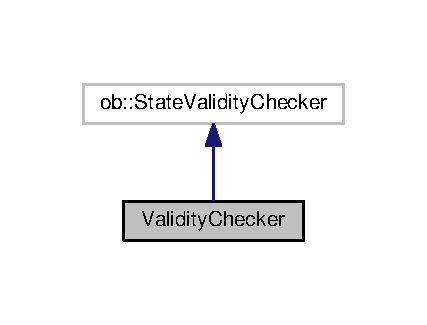
\includegraphics[width=205pt]{classValidityChecker__inherit__graph}
\end{center}
\end{figure}


Collaboration diagram for Validity\+Checker\+:\nopagebreak
\begin{figure}[H]
\begin{center}
\leavevmode
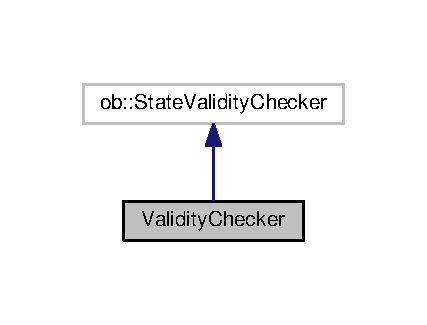
\includegraphics[width=205pt]{classValidityChecker__coll__graph}
\end{center}
\end{figure}
\subsection*{Public Member Functions}
\begin{DoxyCompactItemize}
\item 
\hyperlink{classValidityChecker_ada15197ab56e9e0002e2b11ccac01253}{Validity\+Checker} (const ob\+::\+Space\+Information\+Ptr \&si, std\+::vector$<$ \hyperlink{utils_8hpp_a18281038c49470960bd8f4d15b893441}{Polygon} $>$ obstacle\+\_\+list)
\begin{DoxyCompactList}\small\item\em Constructor. \end{DoxyCompactList}\item 
bool \hyperlink{classValidityChecker_aed770a601b4856c6f055a70ea752be37}{is\+Valid} (const ob\+::\+State $\ast$state) const override
\begin{DoxyCompactList}\small\item\em to check if state is valid of not \end{DoxyCompactList}\end{DoxyCompactItemize}
\subsection*{Public Attributes}
\begin{DoxyCompactItemize}
\item 
std\+::vector$<$ \hyperlink{utils_8hpp_a18281038c49470960bd8f4d15b893441}{Polygon} $>$ \hyperlink{classValidityChecker_a3680b7a8c6e1d6dbaf7833df9f86ce84}{obstacles}
\end{DoxyCompactItemize}


\subsection{Detailed Description}
Class to check if new random state is valid or not. 

\subsection{Constructor \& Destructor Documentation}
\index{Validity\+Checker@{Validity\+Checker}!Validity\+Checker@{Validity\+Checker}}
\index{Validity\+Checker@{Validity\+Checker}!Validity\+Checker@{Validity\+Checker}}
\subsubsection[{\texorpdfstring{Validity\+Checker(const ob\+::\+Space\+Information\+Ptr \&si, std\+::vector$<$ Polygon $>$ obstacle\+\_\+list)}{ValidityChecker(const ob::SpaceInformationPtr &si, std::vector< Polygon > obstacle_list)}}]{\setlength{\rightskip}{0pt plus 5cm}Validity\+Checker\+::\+Validity\+Checker (
\begin{DoxyParamCaption}
\item[{const ob\+::\+Space\+Information\+Ptr \&}]{si, }
\item[{std\+::vector$<$ {\bf Polygon} $>$}]{obstacle\+\_\+list}
\end{DoxyParamCaption}
)\hspace{0.3cm}{\ttfamily [inline]}}\hypertarget{classValidityChecker_ada15197ab56e9e0002e2b11ccac01253}{}\label{classValidityChecker_ada15197ab56e9e0002e2b11ccac01253}


Constructor. 


\begin{DoxyParams}{Parameters}
{\em obstacle\+\_\+list} & Obstacle list that is obtained from map \\
\hline
\end{DoxyParams}


\subsection{Member Function Documentation}
\index{Validity\+Checker@{Validity\+Checker}!is\+Valid@{is\+Valid}}
\index{is\+Valid@{is\+Valid}!Validity\+Checker@{Validity\+Checker}}
\subsubsection[{\texorpdfstring{is\+Valid(const ob\+::\+State $\ast$state) const override}{isValid(const ob::State *state) const override}}]{\setlength{\rightskip}{0pt plus 5cm}bool Validity\+Checker\+::is\+Valid (
\begin{DoxyParamCaption}
\item[{const ob\+::\+State $\ast$}]{state}
\end{DoxyParamCaption}
) const\hspace{0.3cm}{\ttfamily [inline]}, {\ttfamily [override]}}\hypertarget{classValidityChecker_aed770a601b4856c6f055a70ea752be37}{}\label{classValidityChecker_aed770a601b4856c6f055a70ea752be37}


to check if state is valid of not 

Check if new obatined state is inside the obstacle polygon, convert new state to boost point and also polygon to boost polygon and use boost\+::within() method to check the validity of state 
\begin{DoxyParams}{Parameters}
{\em state} & new state that is generated randomly by R\+RT Star algorithm \\
\hline
\end{DoxyParams}
\begin{DoxyReturn}{Returns}
true/false based on the validity of state 
\end{DoxyReturn}


\subsection{Member Data Documentation}
\index{Validity\+Checker@{Validity\+Checker}!obstacles@{obstacles}}
\index{obstacles@{obstacles}!Validity\+Checker@{Validity\+Checker}}
\subsubsection[{\texorpdfstring{obstacles}{obstacles}}]{\setlength{\rightskip}{0pt plus 5cm}std\+::vector$<${\bf Polygon}$>$ Validity\+Checker\+::obstacles}\hypertarget{classValidityChecker_a3680b7a8c6e1d6dbaf7833df9f86ce84}{}\label{classValidityChecker_a3680b7a8c6e1d6dbaf7833df9f86ce84}


The documentation for this class was generated from the following file\+:\begin{DoxyCompactItemize}
\item 
include/\hyperlink{ompl__planning_8hpp}{ompl\+\_\+planning.\+hpp}\end{DoxyCompactItemize}

\chapter{File Documentation}
\hypertarget{dubins__local_8h}{}\section{include/dubins\+\_\+local.h File Reference}
\label{dubins__local_8h}\index{include/dubins\+\_\+local.\+h@{include/dubins\+\_\+local.\+h}}


Contains function declaration related to dubins planner.  


{\ttfamily \#include $<$vector$>$}\\*
{\ttfamily \#include \char`\"{}utils.\+hpp\char`\"{}}\\*
Include dependency graph for dubins\+\_\+local.\+h\+:\nopagebreak
\begin{figure}[H]
\begin{center}
\leavevmode
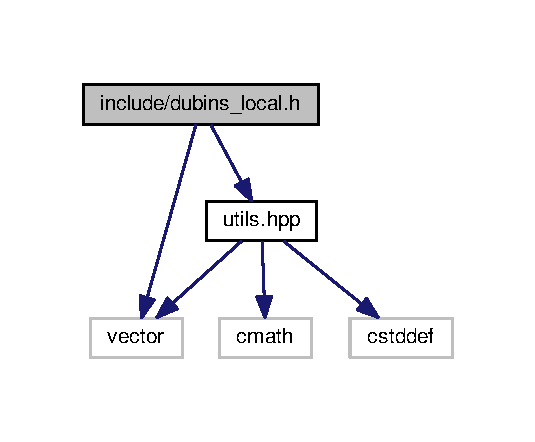
\includegraphics[width=257pt]{dubins__local_8h__incl}
\end{center}
\end{figure}
This graph shows which files directly or indirectly include this file\+:\nopagebreak
\begin{figure}[H]
\begin{center}
\leavevmode
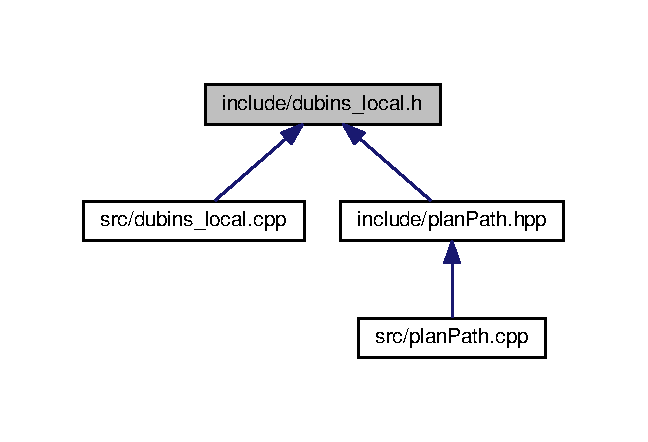
\includegraphics[width=311pt]{dubins__local_8h__dep__incl}
\end{center}
\end{figure}
\subsection*{Classes}
\begin{DoxyCompactItemize}
\item 
struct \hyperlink{structdubinsArc}{dubins\+Arc}
\begin{DoxyCompactList}\small\item\em Structure for a Dubins arc. \end{DoxyCompactList}\item 
struct \hyperlink{structdubinsCurve}{dubins\+Curve}
\begin{DoxyCompactList}\small\item\em Structure for a Dubins curve. \end{DoxyCompactList}\end{DoxyCompactItemize}
\subsection*{Functions}
\begin{DoxyCompactItemize}
\item 
double \hyperlink{dubins__local_8h_a2678c9ac5e8585534a9c5a2385169324}{sinc} (double t)
\item 
double \hyperlink{dubins__local_8h_a2c708c33a19d61b2cdb44cc19fc6b0d9}{mod2pi} (double ang)
\item 
double \hyperlink{dubins__local_8h_a77b0c223b0d9603e0d04e1e5f7a34ae7}{range\+Symm} (double const \&ang)
\item 
bool \hyperlink{dubins__local_8h_a335d08951d7b2832d6b94e2ed9f16aa2}{check} (double const \&s1, double const \&k0, double const \&s2, double const \&k1, double const \&s3, double const \&k2, double const \&th0, double const \&thf)
\item 
void \hyperlink{dubins__local_8h_a22f9f0695527862db7d80a70c45085a1}{scale\+To\+Standard} (double x0, double y0, double th0, double xf, double yf, double thf, double kmax, double \&sc\+\_\+th0, double \&sc\+\_\+thf, double \&sc\+\_\+kmax, double \&lambda)
\item 
void \hyperlink{dubins__local_8h_a217a3380289b2212b7d4bed290541038}{scale\+From\+Standard} (double lambda, double sc\+\_\+s1, double sc\+\_\+s2, double sc\+\_\+s3, double \&s1, double \&s2, double \&s3)
\item 
void \hyperlink{dubins__local_8h_a0d2c667a4f85bd138f5bbe49c21295ca}{L\+SL} (double sc\+\_\+th0, double sc\+\_\+thf, double sc\+\_\+kmax, bool \&ok, double \&sc\+\_\+s1, double \&sc\+\_\+s2, double \&sc\+\_\+s3)
\begin{DoxyCompactList}\small\item\em Compute the arcs for L\+SL configuration. \end{DoxyCompactList}\item 
void \hyperlink{dubins__local_8h_a0bae7f9e0e9f1263038e26b339aef3d8}{R\+SR} (double sc\+\_\+th0, double sc\+\_\+thf, double sc\+\_\+kmax, bool \&ok, double \&sc\+\_\+s1, double \&sc\+\_\+s2, double \&sc\+\_\+s3)
\begin{DoxyCompactList}\small\item\em Compute the arcs for R\+SR configuration. \end{DoxyCompactList}\item 
void \hyperlink{dubins__local_8h_a2b83bd738c98a5adbd9b2f988f83df9b}{L\+SR} (double sc\+\_\+th0, double sc\+\_\+thf, double sc\+\_\+kmax, bool \&ok, double \&sc\+\_\+s1, double \&sc\+\_\+s2, double \&sc\+\_\+s3)
\begin{DoxyCompactList}\small\item\em Compute the arcs for L\+SR configuration. \end{DoxyCompactList}\item 
void \hyperlink{dubins__local_8h_a42faf356426f58054d755d9c4c7dfeaa}{R\+SL} (double sc\+\_\+th0, double sc\+\_\+thf, double sc\+\_\+kmax, bool \&ok, double \&sc\+\_\+s1, double \&sc\+\_\+s2, double \&sc\+\_\+s3)
\begin{DoxyCompactList}\small\item\em Compute the arcs for R\+SL configuration. \end{DoxyCompactList}\item 
void \hyperlink{dubins__local_8h_a321ba579c7cd4b08e84fc34b1d1cdc88}{R\+LR} (double sc\+\_\+th0, double sc\+\_\+thf, double sc\+\_\+kmax, bool \&ok, double \&sc\+\_\+s1, double \&sc\+\_\+s2, double \&sc\+\_\+s3)
\begin{DoxyCompactList}\small\item\em Compute the arcs for R\+LR configuration. \end{DoxyCompactList}\item 
void \hyperlink{dubins__local_8h_a6e4414f09fbd1b41d8879589085585c6}{L\+RL} (double sc\+\_\+th0, double sc\+\_\+thf, double sc\+\_\+kmax, bool \&ok, double \&sc\+\_\+s1, double \&sc\+\_\+s2, double \&sc\+\_\+s3)
\begin{DoxyCompactList}\small\item\em Compute the arcs for L\+RL configuration. \end{DoxyCompactList}\item 
void \hyperlink{dubins__local_8h_aa84b2a5a76850d416eb5b3b238d8a0bc}{set\+\_\+dubins\+Arc} (\hyperlink{structdubinsArc}{dubins\+Arc} \&ptr, double x0, double y0, double th0, double k, double s)
\item 
void \hyperlink{dubins__local_8h_a70c63acda3975bd7bcabdf063fe19b05}{set\+\_\+dubins\+Curve} (\hyperlink{structdubinsCurve}{dubins\+Curve} \&curve\+\_\+ptr, double x0, double y0, double th0, double s1, double s2, double s3, double k0, double k1, double k2)
\item 
void \hyperlink{dubins__local_8h_ab13990cb925d60c2d636ef7ef119865e}{dubins\+\_\+shortest\+\_\+path} (\hyperlink{structdubinsCurve}{dubins\+Curve} \&curve, double const \&x0, double const \&y0, double const \&th0, double const \&xf, double const \&yf, double const \&thf, double const \&kmax)
\begin{DoxyCompactList}\small\item\em Compute shortest path using dunins confiuration. \end{DoxyCompactList}\item 
\hyperlink{structPath}{Path} \hyperlink{dubins__local_8h_a66f54790bf27e578ba9b864ae34de96d}{get\+Path} (\hyperlink{structdubinsCurve}{dubins\+Curve} curve, int npts)
\begin{DoxyCompactList}\small\item\em Discretize the dubins curve to points. \end{DoxyCompactList}\end{DoxyCompactItemize}


\subsection{Detailed Description}
Contains function declaration related to dubins planner. 

\begin{DoxyAuthor}{Author}
Aravind Swaminathan 
\end{DoxyAuthor}
\begin{DoxyDate}{Date}
10-\/\+Jan-\/2020 
\end{DoxyDate}


\subsection{Function Documentation}
\index{dubins\+\_\+local.\+h@{dubins\+\_\+local.\+h}!check@{check}}
\index{check@{check}!dubins\+\_\+local.\+h@{dubins\+\_\+local.\+h}}
\subsubsection[{\texorpdfstring{check(double const \&s1, double const \&k0, double const \&s2, double const \&k1, double const \&s3, double const \&k2, double const \&th0, double const \&thf)}{check(double const &s1, double const &k0, double const &s2, double const &k1, double const &s3, double const &k2, double const &th0, double const &thf)}}]{\setlength{\rightskip}{0pt plus 5cm}bool check (
\begin{DoxyParamCaption}
\item[{double const \&}]{s1, }
\item[{double const \&}]{k0, }
\item[{double const \&}]{s2, }
\item[{double const \&}]{k1, }
\item[{double const \&}]{s3, }
\item[{double const \&}]{k2, }
\item[{double const \&}]{th0, }
\item[{double const \&}]{thf}
\end{DoxyParamCaption}
)}\hypertarget{dubins__local_8h_a335d08951d7b2832d6b94e2ed9f16aa2}{}\label{dubins__local_8h_a335d08951d7b2832d6b94e2ed9f16aa2}
\index{dubins\+\_\+local.\+h@{dubins\+\_\+local.\+h}!dubins\+\_\+shortest\+\_\+path@{dubins\+\_\+shortest\+\_\+path}}
\index{dubins\+\_\+shortest\+\_\+path@{dubins\+\_\+shortest\+\_\+path}!dubins\+\_\+local.\+h@{dubins\+\_\+local.\+h}}
\subsubsection[{\texorpdfstring{dubins\+\_\+shortest\+\_\+path(dubins\+Curve \&curve, double const \&x0, double const \&y0, double const \&th0, double const \&xf, double const \&yf, double const \&thf, double const \&kmax)}{dubins_shortest_path(dubinsCurve &curve, double const &x0, double const &y0, double const &th0, double const &xf, double const &yf, double const &thf, double const &kmax)}}]{\setlength{\rightskip}{0pt plus 5cm}void dubins\+\_\+shortest\+\_\+path (
\begin{DoxyParamCaption}
\item[{{\bf dubins\+Curve} \&}]{curve, }
\item[{double const \&}]{x0, }
\item[{double const \&}]{y0, }
\item[{double const \&}]{th0, }
\item[{double const \&}]{xf, }
\item[{double const \&}]{yf, }
\item[{double const \&}]{thf, }
\item[{double const \&}]{kmax}
\end{DoxyParamCaption}
)}\hypertarget{dubins__local_8h_ab13990cb925d60c2d636ef7ef119865e}{}\label{dubins__local_8h_ab13990cb925d60c2d636ef7ef119865e}


Compute shortest path using dunins confiuration. 


\begin{DoxyParams}{Parameters}
{\em curve} & Output curve \\
\hline
{\em x0} & Start location x \\
\hline
{\em y0} & Start location y \\
\hline
{\em th0} & Start location theta \\
\hline
{\em xf} & End location x \\
\hline
{\em yf} & End location y \\
\hline
{\em thf} & End location theta \\
\hline
{\em kmax} & Maximum curvature of the robot \\
\hline
\end{DoxyParams}
\index{dubins\+\_\+local.\+h@{dubins\+\_\+local.\+h}!get\+Path@{get\+Path}}
\index{get\+Path@{get\+Path}!dubins\+\_\+local.\+h@{dubins\+\_\+local.\+h}}
\subsubsection[{\texorpdfstring{get\+Path(dubins\+Curve curve, int npts)}{getPath(dubinsCurve curve, int npts)}}]{\setlength{\rightskip}{0pt plus 5cm}{\bf Path} get\+Path (
\begin{DoxyParamCaption}
\item[{{\bf dubins\+Curve}}]{curve, }
\item[{int}]{npts}
\end{DoxyParamCaption}
)}\hypertarget{dubins__local_8h_a66f54790bf27e578ba9b864ae34de96d}{}\label{dubins__local_8h_a66f54790bf27e578ba9b864ae34de96d}


Discretize the dubins curve to points. 


\begin{DoxyParams}{Parameters}
{\em curve} & The dubins curve obtained \\
\hline
{\em npts} & Number of points for the whole curve \\
\hline
\end{DoxyParams}
\begin{DoxyReturn}{Returns}
Output path structure 
\end{DoxyReturn}
\index{dubins\+\_\+local.\+h@{dubins\+\_\+local.\+h}!L\+RL@{L\+RL}}
\index{L\+RL@{L\+RL}!dubins\+\_\+local.\+h@{dubins\+\_\+local.\+h}}
\subsubsection[{\texorpdfstring{L\+R\+L(double sc\+\_\+th0, double sc\+\_\+thf, double sc\+\_\+kmax, bool \&ok, double \&sc\+\_\+s1, double \&sc\+\_\+s2, double \&sc\+\_\+s3)}{LRL(double sc_th0, double sc_thf, double sc_kmax, bool &ok, double &sc_s1, double &sc_s2, double &sc_s3)}}]{\setlength{\rightskip}{0pt plus 5cm}void L\+RL (
\begin{DoxyParamCaption}
\item[{double}]{sc\+\_\+th0, }
\item[{double}]{sc\+\_\+thf, }
\item[{double}]{sc\+\_\+kmax, }
\item[{bool \&}]{ok, }
\item[{double \&}]{sc\+\_\+s1, }
\item[{double \&}]{sc\+\_\+s2, }
\item[{double \&}]{sc\+\_\+s3}
\end{DoxyParamCaption}
)}\hypertarget{dubins__local_8h_a6e4414f09fbd1b41d8879589085585c6}{}\label{dubins__local_8h_a6e4414f09fbd1b41d8879589085585c6}


Compute the arcs for L\+RL configuration. 


\begin{DoxyParams}{Parameters}
{\em sc\+\_\+th0} & Start theta \\
\hline
{\em sc\+\_\+thf} & Final theta \\
\hline
{\em sc\+\_\+kmax} & Curvature max \\
\hline
{\em ok} & Check if this configuration fits the given input \\
\hline
{\em sc\+\_\+s1} & Arc 1 coeff \\
\hline
{\em sc\+\_\+s2} & Arc 2 coeff \\
\hline
{\em sc\+\_\+s3} & Arc 3 coeff \\
\hline
\end{DoxyParams}
\index{dubins\+\_\+local.\+h@{dubins\+\_\+local.\+h}!L\+SL@{L\+SL}}
\index{L\+SL@{L\+SL}!dubins\+\_\+local.\+h@{dubins\+\_\+local.\+h}}
\subsubsection[{\texorpdfstring{L\+S\+L(double sc\+\_\+th0, double sc\+\_\+thf, double sc\+\_\+kmax, bool \&ok, double \&sc\+\_\+s1, double \&sc\+\_\+s2, double \&sc\+\_\+s3)}{LSL(double sc_th0, double sc_thf, double sc_kmax, bool &ok, double &sc_s1, double &sc_s2, double &sc_s3)}}]{\setlength{\rightskip}{0pt plus 5cm}void L\+SL (
\begin{DoxyParamCaption}
\item[{double}]{sc\+\_\+th0, }
\item[{double}]{sc\+\_\+thf, }
\item[{double}]{sc\+\_\+kmax, }
\item[{bool \&}]{ok, }
\item[{double \&}]{sc\+\_\+s1, }
\item[{double \&}]{sc\+\_\+s2, }
\item[{double \&}]{sc\+\_\+s3}
\end{DoxyParamCaption}
)}\hypertarget{dubins__local_8h_a0d2c667a4f85bd138f5bbe49c21295ca}{}\label{dubins__local_8h_a0d2c667a4f85bd138f5bbe49c21295ca}


Compute the arcs for L\+SL configuration. 


\begin{DoxyParams}{Parameters}
{\em sc\+\_\+th0} & Start theta \\
\hline
{\em sc\+\_\+thf} & Final theta \\
\hline
{\em sc\+\_\+kmax} & Curvature max \\
\hline
{\em ok} & Check if this configuration fits the given input \\
\hline
{\em sc\+\_\+s1} & Arc 1 coeff \\
\hline
{\em sc\+\_\+s2} & Arc 2 coeff \\
\hline
{\em sc\+\_\+s3} & Arc 3 coeff \\
\hline
\end{DoxyParams}
\index{dubins\+\_\+local.\+h@{dubins\+\_\+local.\+h}!L\+SR@{L\+SR}}
\index{L\+SR@{L\+SR}!dubins\+\_\+local.\+h@{dubins\+\_\+local.\+h}}
\subsubsection[{\texorpdfstring{L\+S\+R(double sc\+\_\+th0, double sc\+\_\+thf, double sc\+\_\+kmax, bool \&ok, double \&sc\+\_\+s1, double \&sc\+\_\+s2, double \&sc\+\_\+s3)}{LSR(double sc_th0, double sc_thf, double sc_kmax, bool &ok, double &sc_s1, double &sc_s2, double &sc_s3)}}]{\setlength{\rightskip}{0pt plus 5cm}void L\+SR (
\begin{DoxyParamCaption}
\item[{double}]{sc\+\_\+th0, }
\item[{double}]{sc\+\_\+thf, }
\item[{double}]{sc\+\_\+kmax, }
\item[{bool \&}]{ok, }
\item[{double \&}]{sc\+\_\+s1, }
\item[{double \&}]{sc\+\_\+s2, }
\item[{double \&}]{sc\+\_\+s3}
\end{DoxyParamCaption}
)}\hypertarget{dubins__local_8h_a2b83bd738c98a5adbd9b2f988f83df9b}{}\label{dubins__local_8h_a2b83bd738c98a5adbd9b2f988f83df9b}


Compute the arcs for L\+SR configuration. 


\begin{DoxyParams}{Parameters}
{\em sc\+\_\+th0} & Start theta \\
\hline
{\em sc\+\_\+thf} & Final theta \\
\hline
{\em sc\+\_\+kmax} & Curvature max \\
\hline
{\em ok} & Check if this configuration fits the given input \\
\hline
{\em sc\+\_\+s1} & Arc 1 coeff \\
\hline
{\em sc\+\_\+s2} & Arc 2 coeff \\
\hline
{\em sc\+\_\+s3} & Arc 3 coeff \\
\hline
\end{DoxyParams}
\index{dubins\+\_\+local.\+h@{dubins\+\_\+local.\+h}!mod2pi@{mod2pi}}
\index{mod2pi@{mod2pi}!dubins\+\_\+local.\+h@{dubins\+\_\+local.\+h}}
\subsubsection[{\texorpdfstring{mod2pi(double ang)}{mod2pi(double ang)}}]{\setlength{\rightskip}{0pt plus 5cm}double mod2pi (
\begin{DoxyParamCaption}
\item[{double}]{ang}
\end{DoxyParamCaption}
)}\hypertarget{dubins__local_8h_a2c708c33a19d61b2cdb44cc19fc6b0d9}{}\label{dubins__local_8h_a2c708c33a19d61b2cdb44cc19fc6b0d9}
\index{dubins\+\_\+local.\+h@{dubins\+\_\+local.\+h}!range\+Symm@{range\+Symm}}
\index{range\+Symm@{range\+Symm}!dubins\+\_\+local.\+h@{dubins\+\_\+local.\+h}}
\subsubsection[{\texorpdfstring{range\+Symm(double const \&ang)}{rangeSymm(double const &ang)}}]{\setlength{\rightskip}{0pt plus 5cm}double range\+Symm (
\begin{DoxyParamCaption}
\item[{double const \&}]{ang}
\end{DoxyParamCaption}
)}\hypertarget{dubins__local_8h_a77b0c223b0d9603e0d04e1e5f7a34ae7}{}\label{dubins__local_8h_a77b0c223b0d9603e0d04e1e5f7a34ae7}
\index{dubins\+\_\+local.\+h@{dubins\+\_\+local.\+h}!R\+LR@{R\+LR}}
\index{R\+LR@{R\+LR}!dubins\+\_\+local.\+h@{dubins\+\_\+local.\+h}}
\subsubsection[{\texorpdfstring{R\+L\+R(double sc\+\_\+th0, double sc\+\_\+thf, double sc\+\_\+kmax, bool \&ok, double \&sc\+\_\+s1, double \&sc\+\_\+s2, double \&sc\+\_\+s3)}{RLR(double sc_th0, double sc_thf, double sc_kmax, bool &ok, double &sc_s1, double &sc_s2, double &sc_s3)}}]{\setlength{\rightskip}{0pt plus 5cm}void R\+LR (
\begin{DoxyParamCaption}
\item[{double}]{sc\+\_\+th0, }
\item[{double}]{sc\+\_\+thf, }
\item[{double}]{sc\+\_\+kmax, }
\item[{bool \&}]{ok, }
\item[{double \&}]{sc\+\_\+s1, }
\item[{double \&}]{sc\+\_\+s2, }
\item[{double \&}]{sc\+\_\+s3}
\end{DoxyParamCaption}
)}\hypertarget{dubins__local_8h_a321ba579c7cd4b08e84fc34b1d1cdc88}{}\label{dubins__local_8h_a321ba579c7cd4b08e84fc34b1d1cdc88}


Compute the arcs for R\+LR configuration. 


\begin{DoxyParams}{Parameters}
{\em sc\+\_\+th0} & Start theta \\
\hline
{\em sc\+\_\+thf} & Final theta \\
\hline
{\em sc\+\_\+kmax} & Curvature max \\
\hline
{\em ok} & Check if this configuration fits the given input \\
\hline
{\em sc\+\_\+s1} & Arc 1 coeff \\
\hline
{\em sc\+\_\+s2} & Arc 2 coeff \\
\hline
{\em sc\+\_\+s3} & Arc 3 coeff \\
\hline
\end{DoxyParams}
\index{dubins\+\_\+local.\+h@{dubins\+\_\+local.\+h}!R\+SL@{R\+SL}}
\index{R\+SL@{R\+SL}!dubins\+\_\+local.\+h@{dubins\+\_\+local.\+h}}
\subsubsection[{\texorpdfstring{R\+S\+L(double sc\+\_\+th0, double sc\+\_\+thf, double sc\+\_\+kmax, bool \&ok, double \&sc\+\_\+s1, double \&sc\+\_\+s2, double \&sc\+\_\+s3)}{RSL(double sc_th0, double sc_thf, double sc_kmax, bool &ok, double &sc_s1, double &sc_s2, double &sc_s3)}}]{\setlength{\rightskip}{0pt plus 5cm}void R\+SL (
\begin{DoxyParamCaption}
\item[{double}]{sc\+\_\+th0, }
\item[{double}]{sc\+\_\+thf, }
\item[{double}]{sc\+\_\+kmax, }
\item[{bool \&}]{ok, }
\item[{double \&}]{sc\+\_\+s1, }
\item[{double \&}]{sc\+\_\+s2, }
\item[{double \&}]{sc\+\_\+s3}
\end{DoxyParamCaption}
)}\hypertarget{dubins__local_8h_a42faf356426f58054d755d9c4c7dfeaa}{}\label{dubins__local_8h_a42faf356426f58054d755d9c4c7dfeaa}


Compute the arcs for R\+SL configuration. 


\begin{DoxyParams}{Parameters}
{\em sc\+\_\+th0} & Start theta \\
\hline
{\em sc\+\_\+thf} & Final theta \\
\hline
{\em sc\+\_\+kmax} & Curvature max \\
\hline
{\em ok} & Check if this configuration fits the given input \\
\hline
{\em sc\+\_\+s1} & Arc 1 coeff \\
\hline
{\em sc\+\_\+s2} & Arc 2 coeff \\
\hline
{\em sc\+\_\+s3} & Arc 3 coeff \\
\hline
\end{DoxyParams}
\index{dubins\+\_\+local.\+h@{dubins\+\_\+local.\+h}!R\+SR@{R\+SR}}
\index{R\+SR@{R\+SR}!dubins\+\_\+local.\+h@{dubins\+\_\+local.\+h}}
\subsubsection[{\texorpdfstring{R\+S\+R(double sc\+\_\+th0, double sc\+\_\+thf, double sc\+\_\+kmax, bool \&ok, double \&sc\+\_\+s1, double \&sc\+\_\+s2, double \&sc\+\_\+s3)}{RSR(double sc_th0, double sc_thf, double sc_kmax, bool &ok, double &sc_s1, double &sc_s2, double &sc_s3)}}]{\setlength{\rightskip}{0pt plus 5cm}void R\+SR (
\begin{DoxyParamCaption}
\item[{double}]{sc\+\_\+th0, }
\item[{double}]{sc\+\_\+thf, }
\item[{double}]{sc\+\_\+kmax, }
\item[{bool \&}]{ok, }
\item[{double \&}]{sc\+\_\+s1, }
\item[{double \&}]{sc\+\_\+s2, }
\item[{double \&}]{sc\+\_\+s3}
\end{DoxyParamCaption}
)}\hypertarget{dubins__local_8h_a0bae7f9e0e9f1263038e26b339aef3d8}{}\label{dubins__local_8h_a0bae7f9e0e9f1263038e26b339aef3d8}


Compute the arcs for R\+SR configuration. 


\begin{DoxyParams}{Parameters}
{\em sc\+\_\+th0} & Start theta \\
\hline
{\em sc\+\_\+thf} & Final theta \\
\hline
{\em sc\+\_\+kmax} & Curvature max \\
\hline
{\em ok} & Check if this configuration fits the given input \\
\hline
{\em sc\+\_\+s1} & Arc 1 coeff \\
\hline
{\em sc\+\_\+s2} & Arc 2 coeff \\
\hline
{\em sc\+\_\+s3} & Arc 3 coeff \\
\hline
\end{DoxyParams}
\index{dubins\+\_\+local.\+h@{dubins\+\_\+local.\+h}!scale\+From\+Standard@{scale\+From\+Standard}}
\index{scale\+From\+Standard@{scale\+From\+Standard}!dubins\+\_\+local.\+h@{dubins\+\_\+local.\+h}}
\subsubsection[{\texorpdfstring{scale\+From\+Standard(double lambda, double sc\+\_\+s1, double sc\+\_\+s2, double sc\+\_\+s3, double \&s1, double \&s2, double \&s3)}{scaleFromStandard(double lambda, double sc_s1, double sc_s2, double sc_s3, double &s1, double &s2, double &s3)}}]{\setlength{\rightskip}{0pt plus 5cm}void scale\+From\+Standard (
\begin{DoxyParamCaption}
\item[{double}]{lambda, }
\item[{double}]{sc\+\_\+s1, }
\item[{double}]{sc\+\_\+s2, }
\item[{double}]{sc\+\_\+s3, }
\item[{double \&}]{s1, }
\item[{double \&}]{s2, }
\item[{double \&}]{s3}
\end{DoxyParamCaption}
)}\hypertarget{dubins__local_8h_a217a3380289b2212b7d4bed290541038}{}\label{dubins__local_8h_a217a3380289b2212b7d4bed290541038}
\index{dubins\+\_\+local.\+h@{dubins\+\_\+local.\+h}!scale\+To\+Standard@{scale\+To\+Standard}}
\index{scale\+To\+Standard@{scale\+To\+Standard}!dubins\+\_\+local.\+h@{dubins\+\_\+local.\+h}}
\subsubsection[{\texorpdfstring{scale\+To\+Standard(double x0, double y0, double th0, double xf, double yf, double thf, double kmax, double \&sc\+\_\+th0, double \&sc\+\_\+thf, double \&sc\+\_\+kmax, double \&lambda)}{scaleToStandard(double x0, double y0, double th0, double xf, double yf, double thf, double kmax, double &sc_th0, double &sc_thf, double &sc_kmax, double &lambda)}}]{\setlength{\rightskip}{0pt plus 5cm}void scale\+To\+Standard (
\begin{DoxyParamCaption}
\item[{double}]{x0, }
\item[{double}]{y0, }
\item[{double}]{th0, }
\item[{double}]{xf, }
\item[{double}]{yf, }
\item[{double}]{thf, }
\item[{double}]{kmax, }
\item[{double \&}]{sc\+\_\+th0, }
\item[{double \&}]{sc\+\_\+thf, }
\item[{double \&}]{sc\+\_\+kmax, }
\item[{double \&}]{lambda}
\end{DoxyParamCaption}
)}\hypertarget{dubins__local_8h_a22f9f0695527862db7d80a70c45085a1}{}\label{dubins__local_8h_a22f9f0695527862db7d80a70c45085a1}
\index{dubins\+\_\+local.\+h@{dubins\+\_\+local.\+h}!set\+\_\+dubins\+Arc@{set\+\_\+dubins\+Arc}}
\index{set\+\_\+dubins\+Arc@{set\+\_\+dubins\+Arc}!dubins\+\_\+local.\+h@{dubins\+\_\+local.\+h}}
\subsubsection[{\texorpdfstring{set\+\_\+dubins\+Arc(dubins\+Arc \&ptr, double x0, double y0, double th0, double k, double s)}{set_dubinsArc(dubinsArc &ptr, double x0, double y0, double th0, double k, double s)}}]{\setlength{\rightskip}{0pt plus 5cm}void set\+\_\+dubins\+Arc (
\begin{DoxyParamCaption}
\item[{{\bf dubins\+Arc} \&}]{ptr, }
\item[{double}]{x0, }
\item[{double}]{y0, }
\item[{double}]{th0, }
\item[{double}]{k, }
\item[{double}]{s}
\end{DoxyParamCaption}
)}\hypertarget{dubins__local_8h_aa84b2a5a76850d416eb5b3b238d8a0bc}{}\label{dubins__local_8h_aa84b2a5a76850d416eb5b3b238d8a0bc}
\index{dubins\+\_\+local.\+h@{dubins\+\_\+local.\+h}!set\+\_\+dubins\+Curve@{set\+\_\+dubins\+Curve}}
\index{set\+\_\+dubins\+Curve@{set\+\_\+dubins\+Curve}!dubins\+\_\+local.\+h@{dubins\+\_\+local.\+h}}
\subsubsection[{\texorpdfstring{set\+\_\+dubins\+Curve(dubins\+Curve \&curve\+\_\+ptr, double x0, double y0, double th0, double s1, double s2, double s3, double k0, double k1, double k2)}{set_dubinsCurve(dubinsCurve &curve_ptr, double x0, double y0, double th0, double s1, double s2, double s3, double k0, double k1, double k2)}}]{\setlength{\rightskip}{0pt plus 5cm}void set\+\_\+dubins\+Curve (
\begin{DoxyParamCaption}
\item[{{\bf dubins\+Curve} \&}]{curve\+\_\+ptr, }
\item[{double}]{x0, }
\item[{double}]{y0, }
\item[{double}]{th0, }
\item[{double}]{s1, }
\item[{double}]{s2, }
\item[{double}]{s3, }
\item[{double}]{k0, }
\item[{double}]{k1, }
\item[{double}]{k2}
\end{DoxyParamCaption}
)}\hypertarget{dubins__local_8h_a70c63acda3975bd7bcabdf063fe19b05}{}\label{dubins__local_8h_a70c63acda3975bd7bcabdf063fe19b05}
\index{dubins\+\_\+local.\+h@{dubins\+\_\+local.\+h}!sinc@{sinc}}
\index{sinc@{sinc}!dubins\+\_\+local.\+h@{dubins\+\_\+local.\+h}}
\subsubsection[{\texorpdfstring{sinc(double t)}{sinc(double t)}}]{\setlength{\rightskip}{0pt plus 5cm}double sinc (
\begin{DoxyParamCaption}
\item[{double}]{t}
\end{DoxyParamCaption}
)}\hypertarget{dubins__local_8h_a2678c9ac5e8585534a9c5a2385169324}{}\label{dubins__local_8h_a2678c9ac5e8585534a9c5a2385169324}

\hypertarget{ompl__planning_8hpp}{}\section{include/ompl\+\_\+planning.hpp File Reference}
\label{ompl__planning_8hpp}\index{include/ompl\+\_\+planning.\+hpp@{include/ompl\+\_\+planning.\+hpp}}


Contains most of the Functions related to O\+M\+PL planer.  


{\ttfamily \#include $<$ompl/base/\+Space\+Information.\+h$>$}\\*
{\ttfamily \#include $<$ompl/base/objectives/\+Path\+Length\+Optimization\+Objective.\+h$>$}\\*
{\ttfamily \#include $<$ompl/base/objectives/\+State\+Cost\+Integral\+Objective.\+h$>$}\\*
{\ttfamily \#include $<$ompl/base/objectives/\+Maximize\+Min\+Clearance\+Objective.\+h$>$}\\*
{\ttfamily \#include $<$ompl/base/spaces/\+Real\+Vector\+State\+Space.\+h$>$}\\*
{\ttfamily \#include \char`\"{}ompl/util/\+Console.\+h\char`\"{}}\\*
{\ttfamily \#include $<$ompl/geometric/planners/prm/\+P\+R\+Mstar.\+h$>$}\\*
{\ttfamily \#include $<$ompl/geometric/planners/rrt/\+R\+R\+Tstar.\+h$>$}\\*
{\ttfamily \#include $<$ompl/base/\+Planner\+Data\+Graph.\+h$>$}\\*
{\ttfamily \#include $<$boost/program\+\_\+options.\+hpp$>$}\\*
{\ttfamily \#include $<$boost/algorithm/string.\+hpp$>$}\\*
{\ttfamily \#include $<$boost/graph/adjacency\+\_\+list.\+hpp$>$}\\*
{\ttfamily \#include $<$boost/geometry.\+hpp$>$}\\*
{\ttfamily \#include $<$boost/geometry/geometries/point\+\_\+xy.\+hpp$>$}\\*
{\ttfamily \#include $<$boost/geometry/geometries/polygon.\+hpp$>$}\\*
{\ttfamily \#include $<$boost/geometry/geometries/linestring.\+hpp$>$}\\*
{\ttfamily \#include $<$boost/graph/dijkstra\+\_\+shortest\+\_\+paths.\+hpp$>$}\\*
{\ttfamily \#include $<$memory$>$}\\*
{\ttfamily \#include $<$fstream$>$}\\*
{\ttfamily \#include \char`\"{}utils.\+hpp\char`\"{}}\\*
{\ttfamily \#include $<$iostream$>$}\\*
Include dependency graph for ompl\+\_\+planning.\+hpp\+:\nopagebreak
\begin{figure}[H]
\begin{center}
\leavevmode
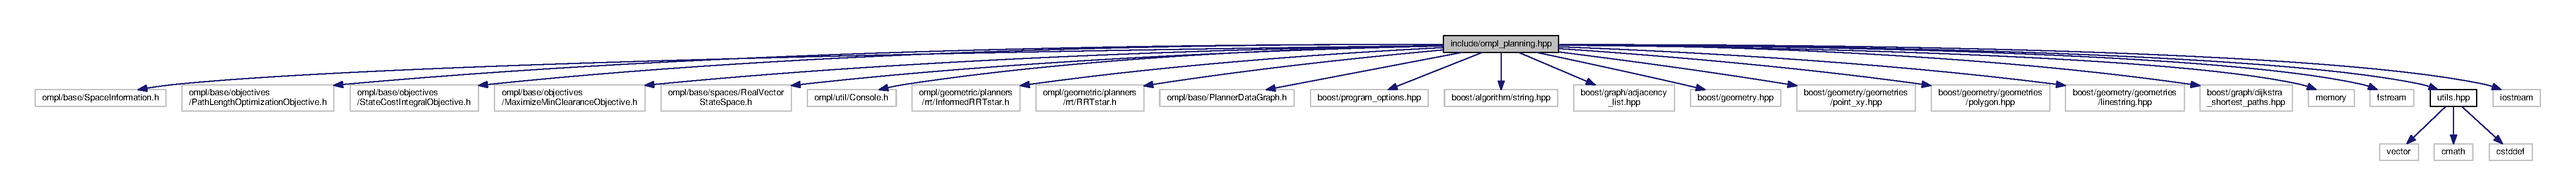
\includegraphics[width=350pt]{ompl__planning_8hpp__incl}
\end{center}
\end{figure}
This graph shows which files directly or indirectly include this file\+:\nopagebreak
\begin{figure}[H]
\begin{center}
\leavevmode
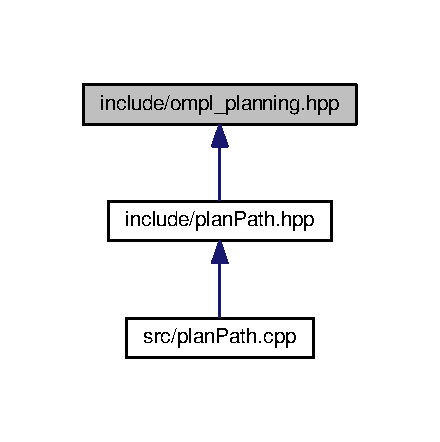
\includegraphics[width=211pt]{ompl__planning_8hpp__dep__incl}
\end{center}
\end{figure}
\subsection*{Classes}
\begin{DoxyCompactItemize}
\item 
class \hyperlink{classClearanceObjective}{Clearance\+Objective}
\item 
class \hyperlink{classValidityChecker}{Validity\+Checker}
\begin{DoxyCompactList}\small\item\em Class to check if new random state is valid or not. \end{DoxyCompactList}\end{DoxyCompactItemize}
\subsection*{Typedefs}
\begin{DoxyCompactItemize}
\item 
typedef bg\+::model\+::d2\+::point\+\_\+xy$<$ double $>$ \hyperlink{ompl__planning_8hpp_a0feb3c557e4cd1e30bb2392478115509}{boost\+\_\+point}
\item 
typedef bg\+::model\+::polygon$<$ \hyperlink{ompl__planning_8hpp_a0feb3c557e4cd1e30bb2392478115509}{boost\+\_\+point} $>$ \hyperlink{ompl__planning_8hpp_a7c1db88611e437728d0bf466e8ad93a2}{boost\+\_\+polygon}
\item 
typedef boost\+::geometry\+::model\+::linestring$<$ \hyperlink{ompl__planning_8hpp_a0feb3c557e4cd1e30bb2392478115509}{boost\+\_\+point} $>$ \hyperlink{ompl__planning_8hpp_ac034f14303d914bba70fd53ec8fcfe35}{boost\+\_\+linestring}
\end{DoxyCompactItemize}
\subsection*{Enumerations}
\begin{DoxyCompactItemize}
\item 
enum \hyperlink{ompl__planning_8hpp_a89a00594ef5f4a0b2ed31d9ede818e45}{optimal\+Planner} \{ \hyperlink{ompl__planning_8hpp_a89a00594ef5f4a0b2ed31d9ede818e45acfe4bd6b555477ccfa326ba4219e89f5}{P\+L\+A\+N\+N\+E\+R\+\_\+\+P\+R\+M\+S\+T\+AR}, 
\hyperlink{ompl__planning_8hpp_a89a00594ef5f4a0b2ed31d9ede818e45ac194e27eeaf4e914b4d4c5715c456ac9}{P\+L\+A\+N\+N\+E\+R\+\_\+\+R\+R\+T\+S\+T\+AR}
 \}\begin{DoxyCompactList}\small\item\em Choice of Optimal planner. \end{DoxyCompactList}
\item 
enum \hyperlink{ompl__planning_8hpp_a536d9a9c9c364afecdce87aaed9c4435}{planning\+Objective} \{ \hyperlink{ompl__planning_8hpp_a536d9a9c9c364afecdce87aaed9c4435adebd4fa82a8cedd6098a31aa2989ad99}{O\+B\+J\+E\+C\+T\+I\+V\+E\+\_\+\+P\+A\+T\+H\+C\+L\+E\+A\+R\+A\+N\+CE}, 
\hyperlink{ompl__planning_8hpp_a536d9a9c9c364afecdce87aaed9c4435a4e3f19a6486ea60fcec03698295bc123}{O\+B\+J\+E\+C\+T\+I\+V\+E\+\_\+\+P\+A\+T\+H\+L\+E\+N\+G\+TH}, 
\hyperlink{ompl__planning_8hpp_a536d9a9c9c364afecdce87aaed9c4435aa2fd04e89b3f63d92aac21da3e830d6e}{O\+B\+J\+E\+C\+T\+I\+V\+E\+\_\+\+T\+H\+R\+E\+S\+H\+O\+L\+D\+P\+A\+T\+H\+L\+E\+N\+G\+TH}, 
\hyperlink{ompl__planning_8hpp_a536d9a9c9c364afecdce87aaed9c4435a6b4f9e0a4cec1bfc91b2dc163dca0cbe}{O\+B\+J\+E\+C\+T\+I\+V\+E\+\_\+\+W\+E\+I\+G\+H\+T\+E\+D\+C\+O\+M\+BO}
 \}\begin{DoxyCompactList}\small\item\em An enum of the supported optimization objectives. \end{DoxyCompactList}
\end{DoxyCompactItemize}
\subsection*{Functions}
\begin{DoxyCompactItemize}
\item 
ob\+::\+Optimization\+Objective\+Ptr \hyperlink{ompl__planning_8hpp_acf18dc373a61806d05ab5bf71ae7e70e}{get\+Path\+Length\+Objective} (const ob\+::\+Space\+Information\+Ptr \&si)
\begin{DoxyCompactList}\small\item\em get path length objective using the space information configured \end{DoxyCompactList}\item 
ob\+::\+Optimization\+Objective\+Ptr \hyperlink{ompl__planning_8hpp_a5a0b977ed1b8de7d5c62fb36bbf60d36}{get\+Threshold\+Path\+Length\+Obj} (const ob\+::\+Space\+Information\+Ptr \&si)
\begin{DoxyCompactList}\small\item\em get path length objective with threshold using the space information configured \end{DoxyCompactList}\item 
ob\+::\+Optimization\+Objective\+Ptr \hyperlink{ompl__planning_8hpp_aaa51340872e046592aa2f59ceb4b0777}{get\+Clearance\+Objective} (const ob\+::\+Space\+Information\+Ptr \&si)
\begin{DoxyCompactList}\small\item\em get Obstace clearance objective using the space information configured \end{DoxyCompactList}\item 
ob\+::\+Optimization\+Objective\+Ptr \hyperlink{ompl__planning_8hpp_af1a62bb9eaa93934c58a4d21eeafb3d6}{get\+Path\+Length\+Obj\+With\+Cost\+To\+Go} (const ob\+::\+Space\+Information\+Ptr \&si)
\begin{DoxyCompactList}\small\item\em get \hyperlink{structPath}{Path} length objective with go to heuristic cost using the space information configured \end{DoxyCompactList}\item 
ob\+::\+Optimization\+Objective\+Ptr \hyperlink{ompl__planning_8hpp_a242e53e3208071455a205daec0352da1}{get\+Balanced\+Objective2} (const ob\+::\+Space\+Information\+Ptr \&si)
\begin{DoxyCompactList}\small\item\em get balanced objective between \hyperlink{structPath}{Path} length optimization and Object clearance \end{DoxyCompactList}\item 
ob\+::\+Optimization\+Objective\+Ptr \hyperlink{ompl__planning_8hpp_a9b35f2b7377808254748d5fe8f415609}{get\+Balanced\+Objective1} (const ob\+::\+Space\+Information\+Ptr \&si)
\begin{DoxyCompactList}\small\item\em get balanced objective between \hyperlink{structPath}{Path} length optimization, Object clearance and Multi Optimization \end{DoxyCompactList}\item 
ob\+::\+Planner\+Ptr \hyperlink{ompl__planning_8hpp_ace8c893484b7db954bc1dd304a217832}{allocate\+Planner} (ob\+::\+Space\+Information\+Ptr si, \hyperlink{ompl__planning_8hpp_a89a00594ef5f4a0b2ed31d9ede818e45}{optimal\+Planner} planner\+Type)
\begin{DoxyCompactList}\small\item\em Allocate planner. \end{DoxyCompactList}\item 
ob\+::\+Optimization\+Objective\+Ptr \hyperlink{ompl__planning_8hpp_a3e0175d952964959806eb2e4b5a3458b}{allocate\+Objective} (const ob\+::\+Space\+Information\+Ptr \&si, \hyperlink{ompl__planning_8hpp_a536d9a9c9c364afecdce87aaed9c4435}{planning\+Objective} objective\+Type)
\begin{DoxyCompactList}\small\item\em Allocate objective. \end{DoxyCompactList}\item 
\hyperlink{ompl__planning_8hpp_a7c1db88611e437728d0bf466e8ad93a2}{boost\+\_\+polygon} \hyperlink{ompl__planning_8hpp_ae9a812e28c680916d034dcf4f3c3b012}{convert\+Polygon\+To\+Boost\+Polygon} (const \hyperlink{utils_8hpp_a18281038c49470960bd8f4d15b893441}{Polygon} \&poly)
\begin{DoxyCompactList}\small\item\em Convert Polygon To Boost polygon. \end{DoxyCompactList}\end{DoxyCompactItemize}


\subsection{Detailed Description}
Contains most of the Functions related to O\+M\+PL planer. 

\begin{DoxyAuthor}{Author}
Aravind Swaminathan 
\end{DoxyAuthor}
\begin{DoxyDate}{Date}
10-\/\+Jan-\/2020 
\end{DoxyDate}


\subsection{Typedef Documentation}
\index{ompl\+\_\+planning.\+hpp@{ompl\+\_\+planning.\+hpp}!boost\+\_\+linestring@{boost\+\_\+linestring}}
\index{boost\+\_\+linestring@{boost\+\_\+linestring}!ompl\+\_\+planning.\+hpp@{ompl\+\_\+planning.\+hpp}}
\subsubsection[{\texorpdfstring{boost\+\_\+linestring}{boost_linestring}}]{\setlength{\rightskip}{0pt plus 5cm}typedef boost\+::geometry\+::model\+::linestring$<${\bf boost\+\_\+point}$>$ {\bf boost\+\_\+linestring}}\hypertarget{ompl__planning_8hpp_ac034f14303d914bba70fd53ec8fcfe35}{}\label{ompl__planning_8hpp_ac034f14303d914bba70fd53ec8fcfe35}
\index{ompl\+\_\+planning.\+hpp@{ompl\+\_\+planning.\+hpp}!boost\+\_\+point@{boost\+\_\+point}}
\index{boost\+\_\+point@{boost\+\_\+point}!ompl\+\_\+planning.\+hpp@{ompl\+\_\+planning.\+hpp}}
\subsubsection[{\texorpdfstring{boost\+\_\+point}{boost_point}}]{\setlength{\rightskip}{0pt plus 5cm}typedef bg\+::model\+::d2\+::point\+\_\+xy$<$double$>$ {\bf boost\+\_\+point}}\hypertarget{ompl__planning_8hpp_a0feb3c557e4cd1e30bb2392478115509}{}\label{ompl__planning_8hpp_a0feb3c557e4cd1e30bb2392478115509}
\index{ompl\+\_\+planning.\+hpp@{ompl\+\_\+planning.\+hpp}!boost\+\_\+polygon@{boost\+\_\+polygon}}
\index{boost\+\_\+polygon@{boost\+\_\+polygon}!ompl\+\_\+planning.\+hpp@{ompl\+\_\+planning.\+hpp}}
\subsubsection[{\texorpdfstring{boost\+\_\+polygon}{boost_polygon}}]{\setlength{\rightskip}{0pt plus 5cm}typedef bg\+::model\+::polygon$<${\bf boost\+\_\+point}$>$ {\bf boost\+\_\+polygon}}\hypertarget{ompl__planning_8hpp_a7c1db88611e437728d0bf466e8ad93a2}{}\label{ompl__planning_8hpp_a7c1db88611e437728d0bf466e8ad93a2}


\subsection{Enumeration Type Documentation}
\index{ompl\+\_\+planning.\+hpp@{ompl\+\_\+planning.\+hpp}!optimal\+Planner@{optimal\+Planner}}
\index{optimal\+Planner@{optimal\+Planner}!ompl\+\_\+planning.\+hpp@{ompl\+\_\+planning.\+hpp}}
\subsubsection[{\texorpdfstring{optimal\+Planner}{optimalPlanner}}]{\setlength{\rightskip}{0pt plus 5cm}enum {\bf optimal\+Planner}}\hypertarget{ompl__planning_8hpp_a89a00594ef5f4a0b2ed31d9ede818e45}{}\label{ompl__planning_8hpp_a89a00594ef5f4a0b2ed31d9ede818e45}


Choice of Optimal planner. 

\begin{Desc}
\item[Enumerator]\par
\begin{description}
\index{P\+L\+A\+N\+N\+E\+R\+\_\+\+P\+R\+M\+S\+T\+AR@{P\+L\+A\+N\+N\+E\+R\+\_\+\+P\+R\+M\+S\+T\+AR}!ompl\+\_\+planning.\+hpp@{ompl\+\_\+planning.\+hpp}}\index{ompl\+\_\+planning.\+hpp@{ompl\+\_\+planning.\+hpp}!P\+L\+A\+N\+N\+E\+R\+\_\+\+P\+R\+M\+S\+T\+AR@{P\+L\+A\+N\+N\+E\+R\+\_\+\+P\+R\+M\+S\+T\+AR}}\item[{\em 
P\+L\+A\+N\+N\+E\+R\+\_\+\+P\+R\+M\+S\+T\+AR\hypertarget{ompl__planning_8hpp_a89a00594ef5f4a0b2ed31d9ede818e45acfe4bd6b555477ccfa326ba4219e89f5}{}\label{ompl__planning_8hpp_a89a00594ef5f4a0b2ed31d9ede818e45acfe4bd6b555477ccfa326ba4219e89f5}
}]P\+RM S\+T\+AR implementation. \index{P\+L\+A\+N\+N\+E\+R\+\_\+\+R\+R\+T\+S\+T\+AR@{P\+L\+A\+N\+N\+E\+R\+\_\+\+R\+R\+T\+S\+T\+AR}!ompl\+\_\+planning.\+hpp@{ompl\+\_\+planning.\+hpp}}\index{ompl\+\_\+planning.\+hpp@{ompl\+\_\+planning.\+hpp}!P\+L\+A\+N\+N\+E\+R\+\_\+\+R\+R\+T\+S\+T\+AR@{P\+L\+A\+N\+N\+E\+R\+\_\+\+R\+R\+T\+S\+T\+AR}}\item[{\em 
P\+L\+A\+N\+N\+E\+R\+\_\+\+R\+R\+T\+S\+T\+AR\hypertarget{ompl__planning_8hpp_a89a00594ef5f4a0b2ed31d9ede818e45ac194e27eeaf4e914b4d4c5715c456ac9}{}\label{ompl__planning_8hpp_a89a00594ef5f4a0b2ed31d9ede818e45ac194e27eeaf4e914b4d4c5715c456ac9}
}]R\+RT Star implementation. \end{description}
\end{Desc}
\index{ompl\+\_\+planning.\+hpp@{ompl\+\_\+planning.\+hpp}!planning\+Objective@{planning\+Objective}}
\index{planning\+Objective@{planning\+Objective}!ompl\+\_\+planning.\+hpp@{ompl\+\_\+planning.\+hpp}}
\subsubsection[{\texorpdfstring{planning\+Objective}{planningObjective}}]{\setlength{\rightskip}{0pt plus 5cm}enum {\bf planning\+Objective}}\hypertarget{ompl__planning_8hpp_a536d9a9c9c364afecdce87aaed9c4435}{}\label{ompl__planning_8hpp_a536d9a9c9c364afecdce87aaed9c4435}


An enum of the supported optimization objectives. 

\begin{Desc}
\item[Enumerator]\par
\begin{description}
\index{O\+B\+J\+E\+C\+T\+I\+V\+E\+\_\+\+P\+A\+T\+H\+C\+L\+E\+A\+R\+A\+N\+CE@{O\+B\+J\+E\+C\+T\+I\+V\+E\+\_\+\+P\+A\+T\+H\+C\+L\+E\+A\+R\+A\+N\+CE}!ompl\+\_\+planning.\+hpp@{ompl\+\_\+planning.\+hpp}}\index{ompl\+\_\+planning.\+hpp@{ompl\+\_\+planning.\+hpp}!O\+B\+J\+E\+C\+T\+I\+V\+E\+\_\+\+P\+A\+T\+H\+C\+L\+E\+A\+R\+A\+N\+CE@{O\+B\+J\+E\+C\+T\+I\+V\+E\+\_\+\+P\+A\+T\+H\+C\+L\+E\+A\+R\+A\+N\+CE}}\item[{\em 
O\+B\+J\+E\+C\+T\+I\+V\+E\+\_\+\+P\+A\+T\+H\+C\+L\+E\+A\+R\+A\+N\+CE\hypertarget{ompl__planning_8hpp_a536d9a9c9c364afecdce87aaed9c4435adebd4fa82a8cedd6098a31aa2989ad99}{}\label{ompl__planning_8hpp_a536d9a9c9c364afecdce87aaed9c4435adebd4fa82a8cedd6098a31aa2989ad99}
}]\hyperlink{structPath}{Path} clearance objective. \index{O\+B\+J\+E\+C\+T\+I\+V\+E\+\_\+\+P\+A\+T\+H\+L\+E\+N\+G\+TH@{O\+B\+J\+E\+C\+T\+I\+V\+E\+\_\+\+P\+A\+T\+H\+L\+E\+N\+G\+TH}!ompl\+\_\+planning.\+hpp@{ompl\+\_\+planning.\+hpp}}\index{ompl\+\_\+planning.\+hpp@{ompl\+\_\+planning.\+hpp}!O\+B\+J\+E\+C\+T\+I\+V\+E\+\_\+\+P\+A\+T\+H\+L\+E\+N\+G\+TH@{O\+B\+J\+E\+C\+T\+I\+V\+E\+\_\+\+P\+A\+T\+H\+L\+E\+N\+G\+TH}}\item[{\em 
O\+B\+J\+E\+C\+T\+I\+V\+E\+\_\+\+P\+A\+T\+H\+L\+E\+N\+G\+TH\hypertarget{ompl__planning_8hpp_a536d9a9c9c364afecdce87aaed9c4435a4e3f19a6486ea60fcec03698295bc123}{}\label{ompl__planning_8hpp_a536d9a9c9c364afecdce87aaed9c4435a4e3f19a6486ea60fcec03698295bc123}
}]\hyperlink{structPath}{Path} length objective. \index{O\+B\+J\+E\+C\+T\+I\+V\+E\+\_\+\+T\+H\+R\+E\+S\+H\+O\+L\+D\+P\+A\+T\+H\+L\+E\+N\+G\+TH@{O\+B\+J\+E\+C\+T\+I\+V\+E\+\_\+\+T\+H\+R\+E\+S\+H\+O\+L\+D\+P\+A\+T\+H\+L\+E\+N\+G\+TH}!ompl\+\_\+planning.\+hpp@{ompl\+\_\+planning.\+hpp}}\index{ompl\+\_\+planning.\+hpp@{ompl\+\_\+planning.\+hpp}!O\+B\+J\+E\+C\+T\+I\+V\+E\+\_\+\+T\+H\+R\+E\+S\+H\+O\+L\+D\+P\+A\+T\+H\+L\+E\+N\+G\+TH@{O\+B\+J\+E\+C\+T\+I\+V\+E\+\_\+\+T\+H\+R\+E\+S\+H\+O\+L\+D\+P\+A\+T\+H\+L\+E\+N\+G\+TH}}\item[{\em 
O\+B\+J\+E\+C\+T\+I\+V\+E\+\_\+\+T\+H\+R\+E\+S\+H\+O\+L\+D\+P\+A\+T\+H\+L\+E\+N\+G\+TH\hypertarget{ompl__planning_8hpp_a536d9a9c9c364afecdce87aaed9c4435aa2fd04e89b3f63d92aac21da3e830d6e}{}\label{ompl__planning_8hpp_a536d9a9c9c364afecdce87aaed9c4435aa2fd04e89b3f63d92aac21da3e830d6e}
}]\hyperlink{structPath}{Path} length with threshold based objective. \index{O\+B\+J\+E\+C\+T\+I\+V\+E\+\_\+\+W\+E\+I\+G\+H\+T\+E\+D\+C\+O\+M\+BO@{O\+B\+J\+E\+C\+T\+I\+V\+E\+\_\+\+W\+E\+I\+G\+H\+T\+E\+D\+C\+O\+M\+BO}!ompl\+\_\+planning.\+hpp@{ompl\+\_\+planning.\+hpp}}\index{ompl\+\_\+planning.\+hpp@{ompl\+\_\+planning.\+hpp}!O\+B\+J\+E\+C\+T\+I\+V\+E\+\_\+\+W\+E\+I\+G\+H\+T\+E\+D\+C\+O\+M\+BO@{O\+B\+J\+E\+C\+T\+I\+V\+E\+\_\+\+W\+E\+I\+G\+H\+T\+E\+D\+C\+O\+M\+BO}}\item[{\em 
O\+B\+J\+E\+C\+T\+I\+V\+E\+\_\+\+W\+E\+I\+G\+H\+T\+E\+D\+C\+O\+M\+BO\hypertarget{ompl__planning_8hpp_a536d9a9c9c364afecdce87aaed9c4435a6b4f9e0a4cec1bfc91b2dc163dca0cbe}{}\label{ompl__planning_8hpp_a536d9a9c9c364afecdce87aaed9c4435a6b4f9e0a4cec1bfc91b2dc163dca0cbe}
}]Weighted combination obejctive of all the above three or two. \end{description}
\end{Desc}


\subsection{Function Documentation}
\index{ompl\+\_\+planning.\+hpp@{ompl\+\_\+planning.\+hpp}!allocate\+Objective@{allocate\+Objective}}
\index{allocate\+Objective@{allocate\+Objective}!ompl\+\_\+planning.\+hpp@{ompl\+\_\+planning.\+hpp}}
\subsubsection[{\texorpdfstring{allocate\+Objective(const ob\+::\+Space\+Information\+Ptr \&si, planning\+Objective objective\+Type)}{allocateObjective(const ob::SpaceInformationPtr &si, planningObjective objectiveType)}}]{\setlength{\rightskip}{0pt plus 5cm}ob\+::\+Optimization\+Objective\+Ptr allocate\+Objective (
\begin{DoxyParamCaption}
\item[{const ob\+::\+Space\+Information\+Ptr \&}]{si, }
\item[{{\bf planning\+Objective}}]{objective\+Type}
\end{DoxyParamCaption}
)}\hypertarget{ompl__planning_8hpp_a3e0175d952964959806eb2e4b5a3458b}{}\label{ompl__planning_8hpp_a3e0175d952964959806eb2e4b5a3458b}


Allocate objective. 

Four objectives of planning 
\begin{DoxyParams}{Parameters}
{\em si} & Space information which includes P\+A\+T\+H\+C\+L\+E\+A\+R\+A\+N\+CE, P\+A\+T\+H\+L\+E\+N\+G\+TH, T\+H\+R\+E\+S\+H\+O\+L\+D\+P\+A\+T\+H\+L\+E\+N\+G\+TH, W\+E\+I\+G\+H\+T\+E\+D\+C\+O\+M\+BO \\
\hline
{\em objective\+Type} & Type of Objective to be used \\
\hline
\end{DoxyParams}
\begin{DoxyReturn}{Returns}
Objective Pointer with corresponding planner 
\end{DoxyReturn}
\index{ompl\+\_\+planning.\+hpp@{ompl\+\_\+planning.\+hpp}!allocate\+Planner@{allocate\+Planner}}
\index{allocate\+Planner@{allocate\+Planner}!ompl\+\_\+planning.\+hpp@{ompl\+\_\+planning.\+hpp}}
\subsubsection[{\texorpdfstring{allocate\+Planner(ob\+::\+Space\+Information\+Ptr si, optimal\+Planner planner\+Type)}{allocatePlanner(ob::SpaceInformationPtr si, optimalPlanner plannerType)}}]{\setlength{\rightskip}{0pt plus 5cm}ob\+::\+Planner\+Ptr allocate\+Planner (
\begin{DoxyParamCaption}
\item[{ob\+::\+Space\+Information\+Ptr}]{si, }
\item[{{\bf optimal\+Planner}}]{planner\+Type}
\end{DoxyParamCaption}
)}\hypertarget{ompl__planning_8hpp_ace8c893484b7db954bc1dd304a217832}{}\label{ompl__planning_8hpp_ace8c893484b7db954bc1dd304a217832}


Allocate planner. 

only two types of planner are considered R\+R\+T$\ast$ and P\+R\+M\+\_\+\+R\+R\+T$\ast$ 
\begin{DoxyParams}{Parameters}
{\em si} & Space information \\
\hline
{\em planner\+Type} & Type of planner to be used \\
\hline
\end{DoxyParams}
\begin{DoxyReturn}{Returns}
Planner Pointer with corresponding planner 
\end{DoxyReturn}
\index{ompl\+\_\+planning.\+hpp@{ompl\+\_\+planning.\+hpp}!convert\+Polygon\+To\+Boost\+Polygon@{convert\+Polygon\+To\+Boost\+Polygon}}
\index{convert\+Polygon\+To\+Boost\+Polygon@{convert\+Polygon\+To\+Boost\+Polygon}!ompl\+\_\+planning.\+hpp@{ompl\+\_\+planning.\+hpp}}
\subsubsection[{\texorpdfstring{convert\+Polygon\+To\+Boost\+Polygon(const Polygon \&poly)}{convertPolygonToBoostPolygon(const Polygon &poly)}}]{\setlength{\rightskip}{0pt plus 5cm}{\bf boost\+\_\+polygon} convert\+Polygon\+To\+Boost\+Polygon (
\begin{DoxyParamCaption}
\item[{const {\bf Polygon} \&}]{poly}
\end{DoxyParamCaption}
)}\hypertarget{ompl__planning_8hpp_ae9a812e28c680916d034dcf4f3c3b012}{}\label{ompl__planning_8hpp_ae9a812e28c680916d034dcf4f3c3b012}


Convert Polygon To Boost polygon. 

Interface polygon struct is converted to boost polygon for easy operation 
\begin{DoxyParams}{Parameters}
{\em poly} & Polygon to be converted \\
\hline
\end{DoxyParams}
\begin{DoxyReturn}{Returns}
Boost polygon object 
\end{DoxyReturn}
\index{ompl\+\_\+planning.\+hpp@{ompl\+\_\+planning.\+hpp}!get\+Balanced\+Objective1@{get\+Balanced\+Objective1}}
\index{get\+Balanced\+Objective1@{get\+Balanced\+Objective1}!ompl\+\_\+planning.\+hpp@{ompl\+\_\+planning.\+hpp}}
\subsubsection[{\texorpdfstring{get\+Balanced\+Objective1(const ob\+::\+Space\+Information\+Ptr \&si)}{getBalancedObjective1(const ob::SpaceInformationPtr &si)}}]{\setlength{\rightskip}{0pt plus 5cm}ob\+::\+Optimization\+Objective\+Ptr get\+Balanced\+Objective1 (
\begin{DoxyParamCaption}
\item[{const ob\+::\+Space\+Information\+Ptr \&}]{si}
\end{DoxyParamCaption}
)}\hypertarget{ompl__planning_8hpp_a9b35f2b7377808254748d5fe8f415609}{}\label{ompl__planning_8hpp_a9b35f2b7377808254748d5fe8f415609}


get balanced objective between \hyperlink{structPath}{Path} length optimization, Object clearance and Multi Optimization 


\begin{DoxyParams}{Parameters}
{\em si} & Space information \\
\hline
\end{DoxyParams}
\begin{DoxyReturn}{Returns}
Optimization objective pointer 
\end{DoxyReturn}
\index{ompl\+\_\+planning.\+hpp@{ompl\+\_\+planning.\+hpp}!get\+Balanced\+Objective2@{get\+Balanced\+Objective2}}
\index{get\+Balanced\+Objective2@{get\+Balanced\+Objective2}!ompl\+\_\+planning.\+hpp@{ompl\+\_\+planning.\+hpp}}
\subsubsection[{\texorpdfstring{get\+Balanced\+Objective2(const ob\+::\+Space\+Information\+Ptr \&si)}{getBalancedObjective2(const ob::SpaceInformationPtr &si)}}]{\setlength{\rightskip}{0pt plus 5cm}ob\+::\+Optimization\+Objective\+Ptr get\+Balanced\+Objective2 (
\begin{DoxyParamCaption}
\item[{const ob\+::\+Space\+Information\+Ptr \&}]{si}
\end{DoxyParamCaption}
)}\hypertarget{ompl__planning_8hpp_a242e53e3208071455a205daec0352da1}{}\label{ompl__planning_8hpp_a242e53e3208071455a205daec0352da1}


get balanced objective between \hyperlink{structPath}{Path} length optimization and Object clearance 


\begin{DoxyParams}{Parameters}
{\em si} & Space information \\
\hline
\end{DoxyParams}
\begin{DoxyReturn}{Returns}
Optimization objective pointer 
\end{DoxyReturn}
\index{ompl\+\_\+planning.\+hpp@{ompl\+\_\+planning.\+hpp}!get\+Clearance\+Objective@{get\+Clearance\+Objective}}
\index{get\+Clearance\+Objective@{get\+Clearance\+Objective}!ompl\+\_\+planning.\+hpp@{ompl\+\_\+planning.\+hpp}}
\subsubsection[{\texorpdfstring{get\+Clearance\+Objective(const ob\+::\+Space\+Information\+Ptr \&si)}{getClearanceObjective(const ob::SpaceInformationPtr &si)}}]{\setlength{\rightskip}{0pt plus 5cm}ob\+::\+Optimization\+Objective\+Ptr get\+Clearance\+Objective (
\begin{DoxyParamCaption}
\item[{const ob\+::\+Space\+Information\+Ptr \&}]{si}
\end{DoxyParamCaption}
)}\hypertarget{ompl__planning_8hpp_aaa51340872e046592aa2f59ceb4b0777}{}\label{ompl__planning_8hpp_aaa51340872e046592aa2f59ceb4b0777}


get Obstace clearance objective using the space information configured 


\begin{DoxyParams}{Parameters}
{\em si} & Space information \\
\hline
\end{DoxyParams}
\begin{DoxyReturn}{Returns}
Optimization objective pointer 
\end{DoxyReturn}
\index{ompl\+\_\+planning.\+hpp@{ompl\+\_\+planning.\+hpp}!get\+Path\+Length\+Objective@{get\+Path\+Length\+Objective}}
\index{get\+Path\+Length\+Objective@{get\+Path\+Length\+Objective}!ompl\+\_\+planning.\+hpp@{ompl\+\_\+planning.\+hpp}}
\subsubsection[{\texorpdfstring{get\+Path\+Length\+Objective(const ob\+::\+Space\+Information\+Ptr \&si)}{getPathLengthObjective(const ob::SpaceInformationPtr &si)}}]{\setlength{\rightskip}{0pt plus 5cm}ob\+::\+Optimization\+Objective\+Ptr get\+Path\+Length\+Objective (
\begin{DoxyParamCaption}
\item[{const ob\+::\+Space\+Information\+Ptr \&}]{si}
\end{DoxyParamCaption}
)}\hypertarget{ompl__planning_8hpp_acf18dc373a61806d05ab5bf71ae7e70e}{}\label{ompl__planning_8hpp_acf18dc373a61806d05ab5bf71ae7e70e}


get path length objective using the space information configured 


\begin{DoxyParams}{Parameters}
{\em si} & Space information \\
\hline
\end{DoxyParams}
\begin{DoxyReturn}{Returns}
Optimization objective pointer 
\end{DoxyReturn}
\index{ompl\+\_\+planning.\+hpp@{ompl\+\_\+planning.\+hpp}!get\+Path\+Length\+Obj\+With\+Cost\+To\+Go@{get\+Path\+Length\+Obj\+With\+Cost\+To\+Go}}
\index{get\+Path\+Length\+Obj\+With\+Cost\+To\+Go@{get\+Path\+Length\+Obj\+With\+Cost\+To\+Go}!ompl\+\_\+planning.\+hpp@{ompl\+\_\+planning.\+hpp}}
\subsubsection[{\texorpdfstring{get\+Path\+Length\+Obj\+With\+Cost\+To\+Go(const ob\+::\+Space\+Information\+Ptr \&si)}{getPathLengthObjWithCostToGo(const ob::SpaceInformationPtr &si)}}]{\setlength{\rightskip}{0pt plus 5cm}ob\+::\+Optimization\+Objective\+Ptr get\+Path\+Length\+Obj\+With\+Cost\+To\+Go (
\begin{DoxyParamCaption}
\item[{const ob\+::\+Space\+Information\+Ptr \&}]{si}
\end{DoxyParamCaption}
)}\hypertarget{ompl__planning_8hpp_af1a62bb9eaa93934c58a4d21eeafb3d6}{}\label{ompl__planning_8hpp_af1a62bb9eaa93934c58a4d21eeafb3d6}


get \hyperlink{structPath}{Path} length objective with go to heuristic cost using the space information configured 


\begin{DoxyParams}{Parameters}
{\em si} & Space information \\
\hline
\end{DoxyParams}
\begin{DoxyReturn}{Returns}
Optimization objective pointer 
\end{DoxyReturn}
\index{ompl\+\_\+planning.\+hpp@{ompl\+\_\+planning.\+hpp}!get\+Threshold\+Path\+Length\+Obj@{get\+Threshold\+Path\+Length\+Obj}}
\index{get\+Threshold\+Path\+Length\+Obj@{get\+Threshold\+Path\+Length\+Obj}!ompl\+\_\+planning.\+hpp@{ompl\+\_\+planning.\+hpp}}
\subsubsection[{\texorpdfstring{get\+Threshold\+Path\+Length\+Obj(const ob\+::\+Space\+Information\+Ptr \&si)}{getThresholdPathLengthObj(const ob::SpaceInformationPtr &si)}}]{\setlength{\rightskip}{0pt plus 5cm}ob\+::\+Optimization\+Objective\+Ptr get\+Threshold\+Path\+Length\+Obj (
\begin{DoxyParamCaption}
\item[{const ob\+::\+Space\+Information\+Ptr \&}]{si}
\end{DoxyParamCaption}
)}\hypertarget{ompl__planning_8hpp_a5a0b977ed1b8de7d5c62fb36bbf60d36}{}\label{ompl__planning_8hpp_a5a0b977ed1b8de7d5c62fb36bbf60d36}


get path length objective with threshold using the space information configured 


\begin{DoxyParams}{Parameters}
{\em si} & Space information \\
\hline
\end{DoxyParams}
\begin{DoxyReturn}{Returns}
Optimization objective pointer 
\end{DoxyReturn}

\hypertarget{planPath_8hpp}{}\section{include/plan\+Path.hpp File Reference}
\label{planPath_8hpp}\index{include/plan\+Path.\+hpp@{include/plan\+Path.\+hpp}}


Contains header inforamtion of plan\+Path functions.  


{\ttfamily \#include \char`\"{}student\+\_\+image\+\_\+elab\+\_\+interface.\+hpp\char`\"{}}\\*
{\ttfamily \#include \char`\"{}student\+\_\+planning\+\_\+interface.\+hpp\char`\"{}}\\*
{\ttfamily \#include $<$stdexcept$>$}\\*
{\ttfamily \#include $<$atomic$>$}\\*
{\ttfamily \#include $<$vector$>$}\\*
{\ttfamily \#include $<$unistd.\+h$>$}\\*
{\ttfamily \#include $<$sstream$>$}\\*
{\ttfamily \#include $<$iostream$>$}\\*
{\ttfamily \#include $<$fstream$>$}\\*
{\ttfamily \#include $<$experimental/filesystem$>$}\\*
{\ttfamily \#include \char`\"{}clipper.\+hpp\char`\"{}}\\*
{\ttfamily \#include \char`\"{}dubins\+\_\+local.\+h\char`\"{}}\\*
{\ttfamily \#include $<$cmath$>$}\\*
{\ttfamily \#include $<$tuple$>$}\\*
{\ttfamily \#include \char`\"{}Clothoids.\+hh\char`\"{}}\\*
{\ttfamily \#include $<$config4cpp/\+Configuration.\+h$>$}\\*
{\ttfamily \#include \char`\"{}rrtstar.\+h\char`\"{}}\\*
{\ttfamily \#include \char`\"{}ompl\+\_\+planning.\+hpp\char`\"{}}\\*
{\ttfamily \#include $<$string$>$}\\*
{\ttfamily \#include $<$chrono$>$}\\*
Include dependency graph for plan\+Path.\+hpp\+:\nopagebreak
\begin{figure}[H]
\begin{center}
\leavevmode
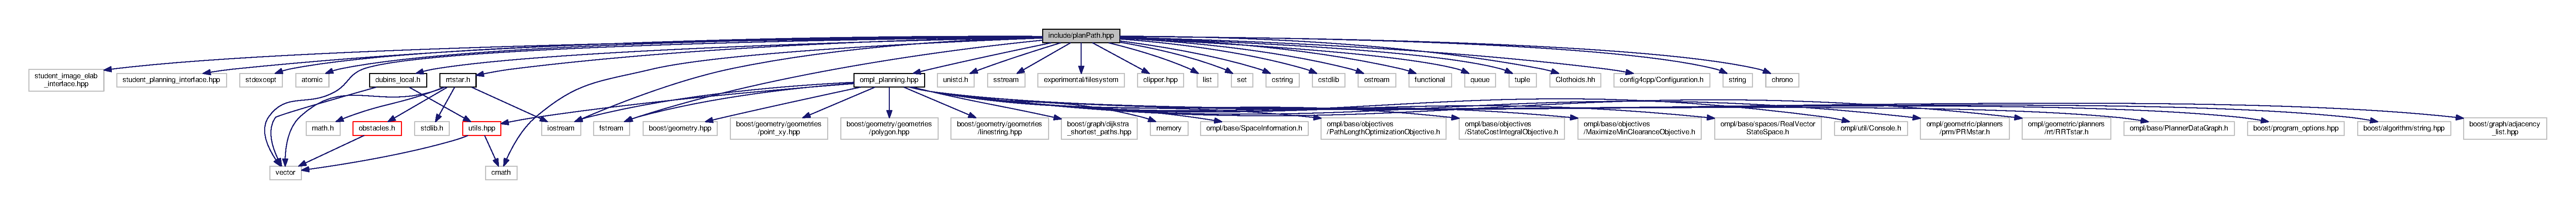
\includegraphics[width=350pt]{planPath_8hpp__incl}
\end{center}
\end{figure}
This graph shows which files directly or indirectly include this file\+:\nopagebreak
\begin{figure}[H]
\begin{center}
\leavevmode
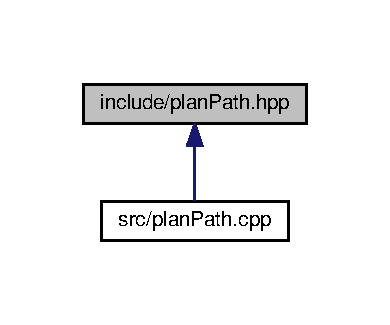
\includegraphics[width=187pt]{planPath_8hpp__dep__incl}
\end{center}
\end{figure}


\subsection{Detailed Description}
Contains header inforamtion of plan\+Path functions. 

\begin{DoxyAuthor}{Author}
Aravind Swaminathan 
\end{DoxyAuthor}
\begin{DoxyDate}{Date}
10-\/\+Jan-\/2020 
\end{DoxyDate}

\hypertarget{README__doxygen_8md}{}\section{R\+E\+A\+D\+M\+E\+\_\+doxygen.\+md File Reference}
\label{README__doxygen_8md}\index{R\+E\+A\+D\+M\+E\+\_\+doxygen.\+md@{R\+E\+A\+D\+M\+E\+\_\+doxygen.\+md}}

\hypertarget{dubins__local_8cpp}{}\section{src/dubins\+\_\+local.cpp File Reference}
\label{dubins__local_8cpp}\index{src/dubins\+\_\+local.\+cpp@{src/dubins\+\_\+local.\+cpp}}


Contains Function definition of dubins local planner.  


{\ttfamily \#include $<$iostream$>$}\\*
{\ttfamily \#include $<$cstdlib$>$}\\*
{\ttfamily \#include $<$vector$>$}\\*
{\ttfamily \#include $<$cmath$>$}\\*
{\ttfamily \#include \char`\"{}dubins\+\_\+local.\+h\char`\"{}}\\*
{\ttfamily \#include \char`\"{}utils.\+hpp\char`\"{}}\\*
Include dependency graph for dubins\+\_\+local.\+cpp\+:\nopagebreak
\begin{figure}[H]
\begin{center}
\leavevmode
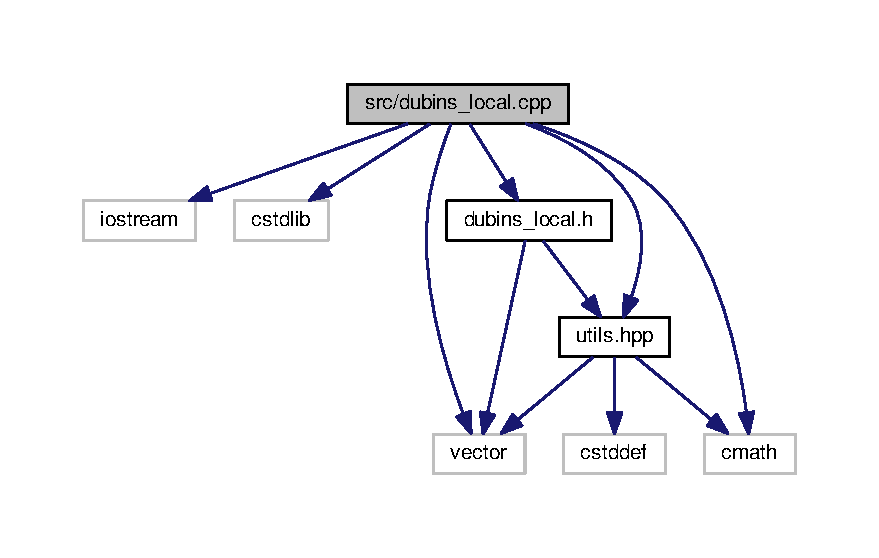
\includegraphics[width=350pt]{dubins__local_8cpp__incl}
\end{center}
\end{figure}
\subsection*{Functions}
\begin{DoxyCompactItemize}
\item 
double \hyperlink{dubins__local_8cpp_a2678c9ac5e8585534a9c5a2385169324}{sinc} (double t)
\item 
double \hyperlink{dubins__local_8cpp_a2c708c33a19d61b2cdb44cc19fc6b0d9}{mod2pi} (double ang)
\item 
double \hyperlink{dubins__local_8cpp_a77b0c223b0d9603e0d04e1e5f7a34ae7}{range\+Symm} (double const \&ang)
\item 
bool \hyperlink{dubins__local_8cpp_a335d08951d7b2832d6b94e2ed9f16aa2}{check} (double const \&s1, double const \&k0, double const \&s2, double const \&k1, double const \&s3, double const \&k2, double const \&th0, double const \&thf)
\item 
void \hyperlink{dubins__local_8cpp_a22f9f0695527862db7d80a70c45085a1}{scale\+To\+Standard} (double x0, double y0, double th0, double xf, double yf, double thf, double kmax, double \&sc\+\_\+th0, double \&sc\+\_\+thf, double \&sc\+\_\+kmax, double \&lambda)
\item 
void \hyperlink{dubins__local_8cpp_a217a3380289b2212b7d4bed290541038}{scale\+From\+Standard} (double lambda, double sc\+\_\+s1, double sc\+\_\+s2, double sc\+\_\+s3, double \&s1, double \&s2, double \&s3)
\item 
void \hyperlink{dubins__local_8cpp_a0d2c667a4f85bd138f5bbe49c21295ca}{L\+SL} (double sc\+\_\+th0, double sc\+\_\+thf, double sc\+\_\+kmax, bool \&ok, double \&sc\+\_\+s1, double \&sc\+\_\+s2, double \&sc\+\_\+s3)
\begin{DoxyCompactList}\small\item\em Compute the arcs for L\+SL configuration. \end{DoxyCompactList}\item 
void \hyperlink{dubins__local_8cpp_a0bae7f9e0e9f1263038e26b339aef3d8}{R\+SR} (double sc\+\_\+th0, double sc\+\_\+thf, double sc\+\_\+kmax, bool \&ok, double \&sc\+\_\+s1, double \&sc\+\_\+s2, double \&sc\+\_\+s3)
\begin{DoxyCompactList}\small\item\em Compute the arcs for R\+SR configuration. \end{DoxyCompactList}\item 
void \hyperlink{dubins__local_8cpp_a2b83bd738c98a5adbd9b2f988f83df9b}{L\+SR} (double sc\+\_\+th0, double sc\+\_\+thf, double sc\+\_\+kmax, bool \&ok, double \&sc\+\_\+s1, double \&sc\+\_\+s2, double \&sc\+\_\+s3)
\begin{DoxyCompactList}\small\item\em Compute the arcs for L\+SR configuration. \end{DoxyCompactList}\item 
void \hyperlink{dubins__local_8cpp_a42faf356426f58054d755d9c4c7dfeaa}{R\+SL} (double sc\+\_\+th0, double sc\+\_\+thf, double sc\+\_\+kmax, bool \&ok, double \&sc\+\_\+s1, double \&sc\+\_\+s2, double \&sc\+\_\+s3)
\begin{DoxyCompactList}\small\item\em Compute the arcs for R\+SL configuration. \end{DoxyCompactList}\item 
void \hyperlink{dubins__local_8cpp_a321ba579c7cd4b08e84fc34b1d1cdc88}{R\+LR} (double sc\+\_\+th0, double sc\+\_\+thf, double sc\+\_\+kmax, bool \&ok, double \&sc\+\_\+s1, double \&sc\+\_\+s2, double \&sc\+\_\+s3)
\begin{DoxyCompactList}\small\item\em Compute the arcs for R\+LR configuration. \end{DoxyCompactList}\item 
void \hyperlink{dubins__local_8cpp_a6e4414f09fbd1b41d8879589085585c6}{L\+RL} (double sc\+\_\+th0, double sc\+\_\+thf, double sc\+\_\+kmax, bool \&ok, double \&sc\+\_\+s1, double \&sc\+\_\+s2, double \&sc\+\_\+s3)
\begin{DoxyCompactList}\small\item\em Compute the arcs for L\+RL configuration. \end{DoxyCompactList}\item 
void \hyperlink{dubins__local_8cpp_aa84b2a5a76850d416eb5b3b238d8a0bc}{set\+\_\+dubins\+Arc} (\hyperlink{structdubinsArc}{dubins\+Arc} \&ptr, double x0, double y0, double th0, double k, double s)
\item 
void \hyperlink{dubins__local_8cpp_a70c63acda3975bd7bcabdf063fe19b05}{set\+\_\+dubins\+Curve} (\hyperlink{structdubinsCurve}{dubins\+Curve} \&curve\+\_\+ptr, double x0, double y0, double th0, double s1, double s2, double s3, double k0, double k1, double k2)
\item 
void \hyperlink{dubins__local_8cpp_ab13990cb925d60c2d636ef7ef119865e}{dubins\+\_\+shortest\+\_\+path} (\hyperlink{structdubinsCurve}{dubins\+Curve} \&curve, double const \&x0, double const \&y0, double const \&th0, double const \&xf, double const \&yf, double const \&thf, double const \&kmax)
\begin{DoxyCompactList}\small\item\em Compute shortest path using dunins confiuration. \end{DoxyCompactList}\item 
\hyperlink{structPath}{Path} \hyperlink{dubins__local_8cpp_a42c439e2e23fcf7d98080a5c68f418ed}{get\+Path} (\hyperlink{structdubinsCurve}{dubins\+Curve} c, int npts)
\begin{DoxyCompactList}\small\item\em Discretize the dubins curve to points. \end{DoxyCompactList}\end{DoxyCompactItemize}


\subsection{Detailed Description}
Contains Function definition of dubins local planner. 

\begin{DoxyAuthor}{Author}
Aravind Swaminathan 
\end{DoxyAuthor}
\begin{DoxyDate}{Date}
10-\/\+Jan-\/2020 
\end{DoxyDate}


\subsection{Function Documentation}
\index{dubins\+\_\+local.\+cpp@{dubins\+\_\+local.\+cpp}!check@{check}}
\index{check@{check}!dubins\+\_\+local.\+cpp@{dubins\+\_\+local.\+cpp}}
\subsubsection[{\texorpdfstring{check(double const \&s1, double const \&k0, double const \&s2, double const \&k1, double const \&s3, double const \&k2, double const \&th0, double const \&thf)}{check(double const &s1, double const &k0, double const &s2, double const &k1, double const &s3, double const &k2, double const &th0, double const &thf)}}]{\setlength{\rightskip}{0pt plus 5cm}bool check (
\begin{DoxyParamCaption}
\item[{double const \&}]{s1, }
\item[{double const \&}]{k0, }
\item[{double const \&}]{s2, }
\item[{double const \&}]{k1, }
\item[{double const \&}]{s3, }
\item[{double const \&}]{k2, }
\item[{double const \&}]{th0, }
\item[{double const \&}]{thf}
\end{DoxyParamCaption}
)}\hypertarget{dubins__local_8cpp_a335d08951d7b2832d6b94e2ed9f16aa2}{}\label{dubins__local_8cpp_a335d08951d7b2832d6b94e2ed9f16aa2}
\index{dubins\+\_\+local.\+cpp@{dubins\+\_\+local.\+cpp}!dubins\+\_\+shortest\+\_\+path@{dubins\+\_\+shortest\+\_\+path}}
\index{dubins\+\_\+shortest\+\_\+path@{dubins\+\_\+shortest\+\_\+path}!dubins\+\_\+local.\+cpp@{dubins\+\_\+local.\+cpp}}
\subsubsection[{\texorpdfstring{dubins\+\_\+shortest\+\_\+path(dubins\+Curve \&curve, double const \&x0, double const \&y0, double const \&th0, double const \&xf, double const \&yf, double const \&thf, double const \&kmax)}{dubins_shortest_path(dubinsCurve &curve, double const &x0, double const &y0, double const &th0, double const &xf, double const &yf, double const &thf, double const &kmax)}}]{\setlength{\rightskip}{0pt plus 5cm}void dubins\+\_\+shortest\+\_\+path (
\begin{DoxyParamCaption}
\item[{{\bf dubins\+Curve} \&}]{curve, }
\item[{double const \&}]{x0, }
\item[{double const \&}]{y0, }
\item[{double const \&}]{th0, }
\item[{double const \&}]{xf, }
\item[{double const \&}]{yf, }
\item[{double const \&}]{thf, }
\item[{double const \&}]{kmax}
\end{DoxyParamCaption}
)}\hypertarget{dubins__local_8cpp_ab13990cb925d60c2d636ef7ef119865e}{}\label{dubins__local_8cpp_ab13990cb925d60c2d636ef7ef119865e}


Compute shortest path using dunins confiuration. 


\begin{DoxyParams}{Parameters}
{\em curve} & Output curve \\
\hline
{\em x0} & Start location x \\
\hline
{\em y0} & Start location y \\
\hline
{\em th0} & Start location theta \\
\hline
{\em xf} & End location x \\
\hline
{\em yf} & End location y \\
\hline
{\em thf} & End location theta \\
\hline
{\em kmax} & Maximum curvature of the robot \\
\hline
\end{DoxyParams}
\index{dubins\+\_\+local.\+cpp@{dubins\+\_\+local.\+cpp}!get\+Path@{get\+Path}}
\index{get\+Path@{get\+Path}!dubins\+\_\+local.\+cpp@{dubins\+\_\+local.\+cpp}}
\subsubsection[{\texorpdfstring{get\+Path(dubins\+Curve c, int npts)}{getPath(dubinsCurve c, int npts)}}]{\setlength{\rightskip}{0pt plus 5cm}{\bf Path} get\+Path (
\begin{DoxyParamCaption}
\item[{{\bf dubins\+Curve}}]{curve, }
\item[{int}]{npts}
\end{DoxyParamCaption}
)}\hypertarget{dubins__local_8cpp_a42c439e2e23fcf7d98080a5c68f418ed}{}\label{dubins__local_8cpp_a42c439e2e23fcf7d98080a5c68f418ed}


Discretize the dubins curve to points. 


\begin{DoxyParams}{Parameters}
{\em curve} & The dubins curve obtained \\
\hline
{\em npts} & Number of points for the whole curve \\
\hline
\end{DoxyParams}
\begin{DoxyReturn}{Returns}
Output path structure 
\end{DoxyReturn}
\index{dubins\+\_\+local.\+cpp@{dubins\+\_\+local.\+cpp}!L\+RL@{L\+RL}}
\index{L\+RL@{L\+RL}!dubins\+\_\+local.\+cpp@{dubins\+\_\+local.\+cpp}}
\subsubsection[{\texorpdfstring{L\+R\+L(double sc\+\_\+th0, double sc\+\_\+thf, double sc\+\_\+kmax, bool \&ok, double \&sc\+\_\+s1, double \&sc\+\_\+s2, double \&sc\+\_\+s3)}{LRL(double sc_th0, double sc_thf, double sc_kmax, bool &ok, double &sc_s1, double &sc_s2, double &sc_s3)}}]{\setlength{\rightskip}{0pt plus 5cm}void L\+RL (
\begin{DoxyParamCaption}
\item[{double}]{sc\+\_\+th0, }
\item[{double}]{sc\+\_\+thf, }
\item[{double}]{sc\+\_\+kmax, }
\item[{bool \&}]{ok, }
\item[{double \&}]{sc\+\_\+s1, }
\item[{double \&}]{sc\+\_\+s2, }
\item[{double \&}]{sc\+\_\+s3}
\end{DoxyParamCaption}
)}\hypertarget{dubins__local_8cpp_a6e4414f09fbd1b41d8879589085585c6}{}\label{dubins__local_8cpp_a6e4414f09fbd1b41d8879589085585c6}


Compute the arcs for L\+RL configuration. 


\begin{DoxyParams}{Parameters}
{\em sc\+\_\+th0} & Start theta \\
\hline
{\em sc\+\_\+thf} & Final theta \\
\hline
{\em sc\+\_\+kmax} & Curvature max \\
\hline
{\em ok} & Check if this configuration fits the given input \\
\hline
{\em sc\+\_\+s1} & Arc 1 coeff \\
\hline
{\em sc\+\_\+s2} & Arc 2 coeff \\
\hline
{\em sc\+\_\+s3} & Arc 3 coeff \\
\hline
\end{DoxyParams}
\index{dubins\+\_\+local.\+cpp@{dubins\+\_\+local.\+cpp}!L\+SL@{L\+SL}}
\index{L\+SL@{L\+SL}!dubins\+\_\+local.\+cpp@{dubins\+\_\+local.\+cpp}}
\subsubsection[{\texorpdfstring{L\+S\+L(double sc\+\_\+th0, double sc\+\_\+thf, double sc\+\_\+kmax, bool \&ok, double \&sc\+\_\+s1, double \&sc\+\_\+s2, double \&sc\+\_\+s3)}{LSL(double sc_th0, double sc_thf, double sc_kmax, bool &ok, double &sc_s1, double &sc_s2, double &sc_s3)}}]{\setlength{\rightskip}{0pt plus 5cm}void L\+SL (
\begin{DoxyParamCaption}
\item[{double}]{sc\+\_\+th0, }
\item[{double}]{sc\+\_\+thf, }
\item[{double}]{sc\+\_\+kmax, }
\item[{bool \&}]{ok, }
\item[{double \&}]{sc\+\_\+s1, }
\item[{double \&}]{sc\+\_\+s2, }
\item[{double \&}]{sc\+\_\+s3}
\end{DoxyParamCaption}
)}\hypertarget{dubins__local_8cpp_a0d2c667a4f85bd138f5bbe49c21295ca}{}\label{dubins__local_8cpp_a0d2c667a4f85bd138f5bbe49c21295ca}


Compute the arcs for L\+SL configuration. 


\begin{DoxyParams}{Parameters}
{\em sc\+\_\+th0} & Start theta \\
\hline
{\em sc\+\_\+thf} & Final theta \\
\hline
{\em sc\+\_\+kmax} & Curvature max \\
\hline
{\em ok} & Check if this configuration fits the given input \\
\hline
{\em sc\+\_\+s1} & Arc 1 coeff \\
\hline
{\em sc\+\_\+s2} & Arc 2 coeff \\
\hline
{\em sc\+\_\+s3} & Arc 3 coeff \\
\hline
\end{DoxyParams}
\index{dubins\+\_\+local.\+cpp@{dubins\+\_\+local.\+cpp}!L\+SR@{L\+SR}}
\index{L\+SR@{L\+SR}!dubins\+\_\+local.\+cpp@{dubins\+\_\+local.\+cpp}}
\subsubsection[{\texorpdfstring{L\+S\+R(double sc\+\_\+th0, double sc\+\_\+thf, double sc\+\_\+kmax, bool \&ok, double \&sc\+\_\+s1, double \&sc\+\_\+s2, double \&sc\+\_\+s3)}{LSR(double sc_th0, double sc_thf, double sc_kmax, bool &ok, double &sc_s1, double &sc_s2, double &sc_s3)}}]{\setlength{\rightskip}{0pt plus 5cm}void L\+SR (
\begin{DoxyParamCaption}
\item[{double}]{sc\+\_\+th0, }
\item[{double}]{sc\+\_\+thf, }
\item[{double}]{sc\+\_\+kmax, }
\item[{bool \&}]{ok, }
\item[{double \&}]{sc\+\_\+s1, }
\item[{double \&}]{sc\+\_\+s2, }
\item[{double \&}]{sc\+\_\+s3}
\end{DoxyParamCaption}
)}\hypertarget{dubins__local_8cpp_a2b83bd738c98a5adbd9b2f988f83df9b}{}\label{dubins__local_8cpp_a2b83bd738c98a5adbd9b2f988f83df9b}


Compute the arcs for L\+SR configuration. 


\begin{DoxyParams}{Parameters}
{\em sc\+\_\+th0} & Start theta \\
\hline
{\em sc\+\_\+thf} & Final theta \\
\hline
{\em sc\+\_\+kmax} & Curvature max \\
\hline
{\em ok} & Check if this configuration fits the given input \\
\hline
{\em sc\+\_\+s1} & Arc 1 coeff \\
\hline
{\em sc\+\_\+s2} & Arc 2 coeff \\
\hline
{\em sc\+\_\+s3} & Arc 3 coeff \\
\hline
\end{DoxyParams}
\index{dubins\+\_\+local.\+cpp@{dubins\+\_\+local.\+cpp}!mod2pi@{mod2pi}}
\index{mod2pi@{mod2pi}!dubins\+\_\+local.\+cpp@{dubins\+\_\+local.\+cpp}}
\subsubsection[{\texorpdfstring{mod2pi(double ang)}{mod2pi(double ang)}}]{\setlength{\rightskip}{0pt plus 5cm}double mod2pi (
\begin{DoxyParamCaption}
\item[{double}]{ang}
\end{DoxyParamCaption}
)}\hypertarget{dubins__local_8cpp_a2c708c33a19d61b2cdb44cc19fc6b0d9}{}\label{dubins__local_8cpp_a2c708c33a19d61b2cdb44cc19fc6b0d9}
\index{dubins\+\_\+local.\+cpp@{dubins\+\_\+local.\+cpp}!range\+Symm@{range\+Symm}}
\index{range\+Symm@{range\+Symm}!dubins\+\_\+local.\+cpp@{dubins\+\_\+local.\+cpp}}
\subsubsection[{\texorpdfstring{range\+Symm(double const \&ang)}{rangeSymm(double const &ang)}}]{\setlength{\rightskip}{0pt plus 5cm}double range\+Symm (
\begin{DoxyParamCaption}
\item[{double const \&}]{ang}
\end{DoxyParamCaption}
)}\hypertarget{dubins__local_8cpp_a77b0c223b0d9603e0d04e1e5f7a34ae7}{}\label{dubins__local_8cpp_a77b0c223b0d9603e0d04e1e5f7a34ae7}
\index{dubins\+\_\+local.\+cpp@{dubins\+\_\+local.\+cpp}!R\+LR@{R\+LR}}
\index{R\+LR@{R\+LR}!dubins\+\_\+local.\+cpp@{dubins\+\_\+local.\+cpp}}
\subsubsection[{\texorpdfstring{R\+L\+R(double sc\+\_\+th0, double sc\+\_\+thf, double sc\+\_\+kmax, bool \&ok, double \&sc\+\_\+s1, double \&sc\+\_\+s2, double \&sc\+\_\+s3)}{RLR(double sc_th0, double sc_thf, double sc_kmax, bool &ok, double &sc_s1, double &sc_s2, double &sc_s3)}}]{\setlength{\rightskip}{0pt plus 5cm}void R\+LR (
\begin{DoxyParamCaption}
\item[{double}]{sc\+\_\+th0, }
\item[{double}]{sc\+\_\+thf, }
\item[{double}]{sc\+\_\+kmax, }
\item[{bool \&}]{ok, }
\item[{double \&}]{sc\+\_\+s1, }
\item[{double \&}]{sc\+\_\+s2, }
\item[{double \&}]{sc\+\_\+s3}
\end{DoxyParamCaption}
)}\hypertarget{dubins__local_8cpp_a321ba579c7cd4b08e84fc34b1d1cdc88}{}\label{dubins__local_8cpp_a321ba579c7cd4b08e84fc34b1d1cdc88}


Compute the arcs for R\+LR configuration. 


\begin{DoxyParams}{Parameters}
{\em sc\+\_\+th0} & Start theta \\
\hline
{\em sc\+\_\+thf} & Final theta \\
\hline
{\em sc\+\_\+kmax} & Curvature max \\
\hline
{\em ok} & Check if this configuration fits the given input \\
\hline
{\em sc\+\_\+s1} & Arc 1 coeff \\
\hline
{\em sc\+\_\+s2} & Arc 2 coeff \\
\hline
{\em sc\+\_\+s3} & Arc 3 coeff \\
\hline
\end{DoxyParams}
\index{dubins\+\_\+local.\+cpp@{dubins\+\_\+local.\+cpp}!R\+SL@{R\+SL}}
\index{R\+SL@{R\+SL}!dubins\+\_\+local.\+cpp@{dubins\+\_\+local.\+cpp}}
\subsubsection[{\texorpdfstring{R\+S\+L(double sc\+\_\+th0, double sc\+\_\+thf, double sc\+\_\+kmax, bool \&ok, double \&sc\+\_\+s1, double \&sc\+\_\+s2, double \&sc\+\_\+s3)}{RSL(double sc_th0, double sc_thf, double sc_kmax, bool &ok, double &sc_s1, double &sc_s2, double &sc_s3)}}]{\setlength{\rightskip}{0pt plus 5cm}void R\+SL (
\begin{DoxyParamCaption}
\item[{double}]{sc\+\_\+th0, }
\item[{double}]{sc\+\_\+thf, }
\item[{double}]{sc\+\_\+kmax, }
\item[{bool \&}]{ok, }
\item[{double \&}]{sc\+\_\+s1, }
\item[{double \&}]{sc\+\_\+s2, }
\item[{double \&}]{sc\+\_\+s3}
\end{DoxyParamCaption}
)}\hypertarget{dubins__local_8cpp_a42faf356426f58054d755d9c4c7dfeaa}{}\label{dubins__local_8cpp_a42faf356426f58054d755d9c4c7dfeaa}


Compute the arcs for R\+SL configuration. 


\begin{DoxyParams}{Parameters}
{\em sc\+\_\+th0} & Start theta \\
\hline
{\em sc\+\_\+thf} & Final theta \\
\hline
{\em sc\+\_\+kmax} & Curvature max \\
\hline
{\em ok} & Check if this configuration fits the given input \\
\hline
{\em sc\+\_\+s1} & Arc 1 coeff \\
\hline
{\em sc\+\_\+s2} & Arc 2 coeff \\
\hline
{\em sc\+\_\+s3} & Arc 3 coeff \\
\hline
\end{DoxyParams}
\index{dubins\+\_\+local.\+cpp@{dubins\+\_\+local.\+cpp}!R\+SR@{R\+SR}}
\index{R\+SR@{R\+SR}!dubins\+\_\+local.\+cpp@{dubins\+\_\+local.\+cpp}}
\subsubsection[{\texorpdfstring{R\+S\+R(double sc\+\_\+th0, double sc\+\_\+thf, double sc\+\_\+kmax, bool \&ok, double \&sc\+\_\+s1, double \&sc\+\_\+s2, double \&sc\+\_\+s3)}{RSR(double sc_th0, double sc_thf, double sc_kmax, bool &ok, double &sc_s1, double &sc_s2, double &sc_s3)}}]{\setlength{\rightskip}{0pt plus 5cm}void R\+SR (
\begin{DoxyParamCaption}
\item[{double}]{sc\+\_\+th0, }
\item[{double}]{sc\+\_\+thf, }
\item[{double}]{sc\+\_\+kmax, }
\item[{bool \&}]{ok, }
\item[{double \&}]{sc\+\_\+s1, }
\item[{double \&}]{sc\+\_\+s2, }
\item[{double \&}]{sc\+\_\+s3}
\end{DoxyParamCaption}
)}\hypertarget{dubins__local_8cpp_a0bae7f9e0e9f1263038e26b339aef3d8}{}\label{dubins__local_8cpp_a0bae7f9e0e9f1263038e26b339aef3d8}


Compute the arcs for R\+SR configuration. 


\begin{DoxyParams}{Parameters}
{\em sc\+\_\+th0} & Start theta \\
\hline
{\em sc\+\_\+thf} & Final theta \\
\hline
{\em sc\+\_\+kmax} & Curvature max \\
\hline
{\em ok} & Check if this configuration fits the given input \\
\hline
{\em sc\+\_\+s1} & Arc 1 coeff \\
\hline
{\em sc\+\_\+s2} & Arc 2 coeff \\
\hline
{\em sc\+\_\+s3} & Arc 3 coeff \\
\hline
\end{DoxyParams}
\index{dubins\+\_\+local.\+cpp@{dubins\+\_\+local.\+cpp}!scale\+From\+Standard@{scale\+From\+Standard}}
\index{scale\+From\+Standard@{scale\+From\+Standard}!dubins\+\_\+local.\+cpp@{dubins\+\_\+local.\+cpp}}
\subsubsection[{\texorpdfstring{scale\+From\+Standard(double lambda, double sc\+\_\+s1, double sc\+\_\+s2, double sc\+\_\+s3, double \&s1, double \&s2, double \&s3)}{scaleFromStandard(double lambda, double sc_s1, double sc_s2, double sc_s3, double &s1, double &s2, double &s3)}}]{\setlength{\rightskip}{0pt plus 5cm}void scale\+From\+Standard (
\begin{DoxyParamCaption}
\item[{double}]{lambda, }
\item[{double}]{sc\+\_\+s1, }
\item[{double}]{sc\+\_\+s2, }
\item[{double}]{sc\+\_\+s3, }
\item[{double \&}]{s1, }
\item[{double \&}]{s2, }
\item[{double \&}]{s3}
\end{DoxyParamCaption}
)}\hypertarget{dubins__local_8cpp_a217a3380289b2212b7d4bed290541038}{}\label{dubins__local_8cpp_a217a3380289b2212b7d4bed290541038}
\index{dubins\+\_\+local.\+cpp@{dubins\+\_\+local.\+cpp}!scale\+To\+Standard@{scale\+To\+Standard}}
\index{scale\+To\+Standard@{scale\+To\+Standard}!dubins\+\_\+local.\+cpp@{dubins\+\_\+local.\+cpp}}
\subsubsection[{\texorpdfstring{scale\+To\+Standard(double x0, double y0, double th0, double xf, double yf, double thf, double kmax, double \&sc\+\_\+th0, double \&sc\+\_\+thf, double \&sc\+\_\+kmax, double \&lambda)}{scaleToStandard(double x0, double y0, double th0, double xf, double yf, double thf, double kmax, double &sc_th0, double &sc_thf, double &sc_kmax, double &lambda)}}]{\setlength{\rightskip}{0pt plus 5cm}void scale\+To\+Standard (
\begin{DoxyParamCaption}
\item[{double}]{x0, }
\item[{double}]{y0, }
\item[{double}]{th0, }
\item[{double}]{xf, }
\item[{double}]{yf, }
\item[{double}]{thf, }
\item[{double}]{kmax, }
\item[{double \&}]{sc\+\_\+th0, }
\item[{double \&}]{sc\+\_\+thf, }
\item[{double \&}]{sc\+\_\+kmax, }
\item[{double \&}]{lambda}
\end{DoxyParamCaption}
)}\hypertarget{dubins__local_8cpp_a22f9f0695527862db7d80a70c45085a1}{}\label{dubins__local_8cpp_a22f9f0695527862db7d80a70c45085a1}
\index{dubins\+\_\+local.\+cpp@{dubins\+\_\+local.\+cpp}!set\+\_\+dubins\+Arc@{set\+\_\+dubins\+Arc}}
\index{set\+\_\+dubins\+Arc@{set\+\_\+dubins\+Arc}!dubins\+\_\+local.\+cpp@{dubins\+\_\+local.\+cpp}}
\subsubsection[{\texorpdfstring{set\+\_\+dubins\+Arc(dubins\+Arc \&ptr, double x0, double y0, double th0, double k, double s)}{set_dubinsArc(dubinsArc &ptr, double x0, double y0, double th0, double k, double s)}}]{\setlength{\rightskip}{0pt plus 5cm}void set\+\_\+dubins\+Arc (
\begin{DoxyParamCaption}
\item[{{\bf dubins\+Arc} \&}]{ptr, }
\item[{double}]{x0, }
\item[{double}]{y0, }
\item[{double}]{th0, }
\item[{double}]{k, }
\item[{double}]{s}
\end{DoxyParamCaption}
)}\hypertarget{dubins__local_8cpp_aa84b2a5a76850d416eb5b3b238d8a0bc}{}\label{dubins__local_8cpp_aa84b2a5a76850d416eb5b3b238d8a0bc}
\index{dubins\+\_\+local.\+cpp@{dubins\+\_\+local.\+cpp}!set\+\_\+dubins\+Curve@{set\+\_\+dubins\+Curve}}
\index{set\+\_\+dubins\+Curve@{set\+\_\+dubins\+Curve}!dubins\+\_\+local.\+cpp@{dubins\+\_\+local.\+cpp}}
\subsubsection[{\texorpdfstring{set\+\_\+dubins\+Curve(dubins\+Curve \&curve\+\_\+ptr, double x0, double y0, double th0, double s1, double s2, double s3, double k0, double k1, double k2)}{set_dubinsCurve(dubinsCurve &curve_ptr, double x0, double y0, double th0, double s1, double s2, double s3, double k0, double k1, double k2)}}]{\setlength{\rightskip}{0pt plus 5cm}void set\+\_\+dubins\+Curve (
\begin{DoxyParamCaption}
\item[{{\bf dubins\+Curve} \&}]{curve\+\_\+ptr, }
\item[{double}]{x0, }
\item[{double}]{y0, }
\item[{double}]{th0, }
\item[{double}]{s1, }
\item[{double}]{s2, }
\item[{double}]{s3, }
\item[{double}]{k0, }
\item[{double}]{k1, }
\item[{double}]{k2}
\end{DoxyParamCaption}
)}\hypertarget{dubins__local_8cpp_a70c63acda3975bd7bcabdf063fe19b05}{}\label{dubins__local_8cpp_a70c63acda3975bd7bcabdf063fe19b05}
\index{dubins\+\_\+local.\+cpp@{dubins\+\_\+local.\+cpp}!sinc@{sinc}}
\index{sinc@{sinc}!dubins\+\_\+local.\+cpp@{dubins\+\_\+local.\+cpp}}
\subsubsection[{\texorpdfstring{sinc(double t)}{sinc(double t)}}]{\setlength{\rightskip}{0pt plus 5cm}double sinc (
\begin{DoxyParamCaption}
\item[{double}]{t}
\end{DoxyParamCaption}
)}\hypertarget{dubins__local_8cpp_a2678c9ac5e8585534a9c5a2385169324}{}\label{dubins__local_8cpp_a2678c9ac5e8585534a9c5a2385169324}

\hypertarget{extrisnicCalib_8cpp}{}\section{src/extrisnic\+Calib.cpp File Reference}
\label{extrisnicCalib_8cpp}\index{src/extrisnic\+Calib.\+cpp@{src/extrisnic\+Calib.\+cpp}}
{\ttfamily \#include \char`\"{}student\+\_\+image\+\_\+elab\+\_\+interface.\+hpp\char`\"{}}\\*
{\ttfamily \#include \char`\"{}student\+\_\+planning\+\_\+interface.\+hpp\char`\"{}}\\*
{\ttfamily \#include $<$stdexcept$>$}\\*
{\ttfamily \#include $<$atomic$>$}\\*
{\ttfamily \#include $<$unistd.\+h$>$}\\*
{\ttfamily \#include $<$sstream$>$}\\*
{\ttfamily \#include $<$experimental/filesystem$>$}\\*
Include dependency graph for extrisnic\+Calib.\+cpp\+:\nopagebreak
\begin{figure}[H]
\begin{center}
\leavevmode
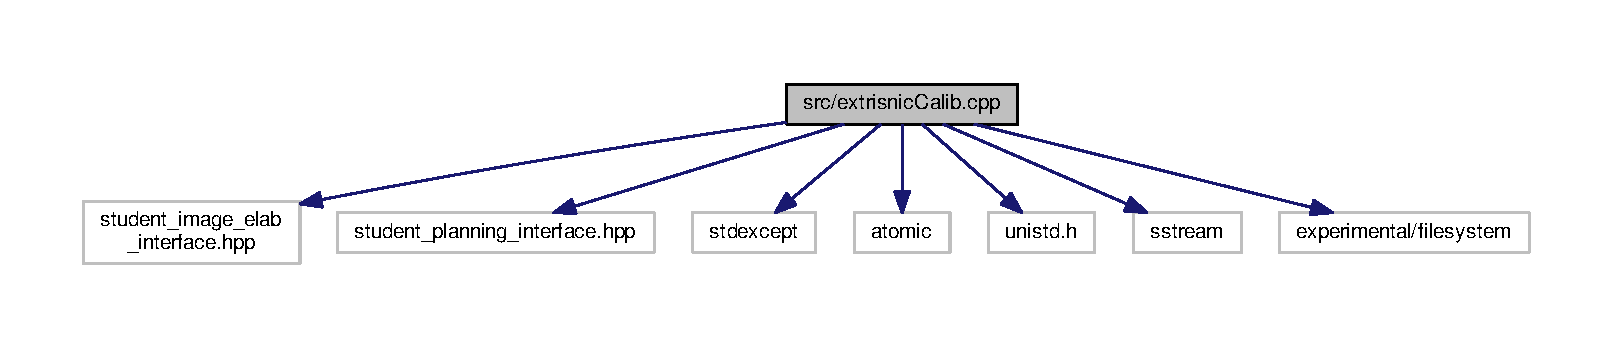
\includegraphics[width=350pt]{extrisnicCalib_8cpp__incl}
\end{center}
\end{figure}
\subsection*{Namespaces}
\begin{DoxyCompactItemize}
\item 
 \hyperlink{namespacestudent}{student}
\end{DoxyCompactItemize}
\subsection*{Functions}
\begin{DoxyCompactItemize}
\item 
void \hyperlink{namespacestudent_ab3f1d6c8dd4caa817efc0cd3c46eb2e0}{student\+::mouse\+Callback} (int event, int x, int y, int, void $\ast$p)
\begin{DoxyCompactList}\small\item\em Function called after every mouse click. \end{DoxyCompactList}\item 
std\+::vector$<$ cv\+::\+Point2f $>$ \hyperlink{namespacestudent_a01244e0e0a28d974de100ffcad7a2583}{student\+::pick\+N\+Points} (int n0, const cv\+::\+Mat \&img)
\begin{DoxyCompactList}\small\item\em Function to pick points from image. \end{DoxyCompactList}\item 
bool \hyperlink{namespacestudent_a6103f938ce28f8820c48c089d5f95098}{student\+::extrinsic\+Calib} (const cv\+::\+Mat \&img\+\_\+in, std\+::vector$<$ cv\+::\+Point3f $>$ object\+\_\+points, const cv\+::\+Mat \&camera\+\_\+matrix, cv\+::\+Mat \&rvec, cv\+::\+Mat \&tvec, const std\+::string \&config\+\_\+folder)
\begin{DoxyCompactList}\small\item\em Function for extrinsic calibration. \end{DoxyCompactList}\item 
void \hyperlink{namespacestudent_aceb2a29362b8223a9d3601d9496e1c98}{student\+::image\+Undistort} (const cv\+::\+Mat \&img\+\_\+in, cv\+::\+Mat \&img\+\_\+out, const cv\+::\+Mat \&cam\+\_\+matrix, const cv\+::\+Mat \&dist\+\_\+coeffs, const std\+::string \&config\+\_\+folder)
\begin{DoxyCompactList}\small\item\em Function undistort the given image. \end{DoxyCompactList}\item 
void \hyperlink{namespacestudent_a528d33658d0d4d982a46f18b7abb4a70}{student\+::find\+Plane\+Transform} (const cv\+::\+Mat \&cam\+\_\+matrix, const cv\+::\+Mat \&rvec, const cv\+::\+Mat \&tvec, const std\+::vector$<$ cv\+::\+Point3f $>$ \&object\+\_\+points\+\_\+plane, const std\+::vector$<$ cv\+::\+Point2f $>$ \&dest\+\_\+image\+\_\+points\+\_\+plane, cv\+::\+Mat \&plane\+\_\+transf, const std\+::string \&config\+\_\+folder)
\begin{DoxyCompactList}\small\item\em Perspective projection. \end{DoxyCompactList}\item 
void \hyperlink{namespacestudent_a6b8caf348979f55e58a75193233c219d}{student\+::unwarp} (const cv\+::\+Mat \&img\+\_\+in, cv\+::\+Mat \&img\+\_\+out, const cv\+::\+Mat \&transf, const std\+::string \&config\+\_\+folder)
\begin{DoxyCompactList}\small\item\em Image unwarping. \end{DoxyCompactList}\end{DoxyCompactItemize}
\subsection*{Variables}
\begin{DoxyCompactItemize}
\item 
cv\+::\+Mat \hyperlink{namespacestudent_a65fee22a07178fcde6362c2482b5fa7f}{student\+::dist\+\_\+coeffs\+\_\+for\+\_\+ex}
\end{DoxyCompactItemize}

\hypertarget{findRobot_8cpp}{}\section{src/find\+Robot.cpp File Reference}
\label{findRobot_8cpp}\index{src/find\+Robot.\+cpp@{src/find\+Robot.\+cpp}}
{\ttfamily \#include \char`\"{}student\+\_\+image\+\_\+elab\+\_\+interface.\+hpp\char`\"{}}\\*
{\ttfamily \#include \char`\"{}student\+\_\+planning\+\_\+interface.\+hpp\char`\"{}}\\*
{\ttfamily \#include $<$stdexcept$>$}\\*
{\ttfamily \#include $<$atomic$>$}\\*
{\ttfamily \#include $<$unistd.\+h$>$}\\*
{\ttfamily \#include $<$sstream$>$}\\*
{\ttfamily \#include $<$experimental/filesystem$>$}\\*
{\ttfamily \#include $<$config4cpp/\+Configuration.\+h$>$}\\*
Include dependency graph for find\+Robot.\+cpp\+:\nopagebreak
\begin{figure}[H]
\begin{center}
\leavevmode
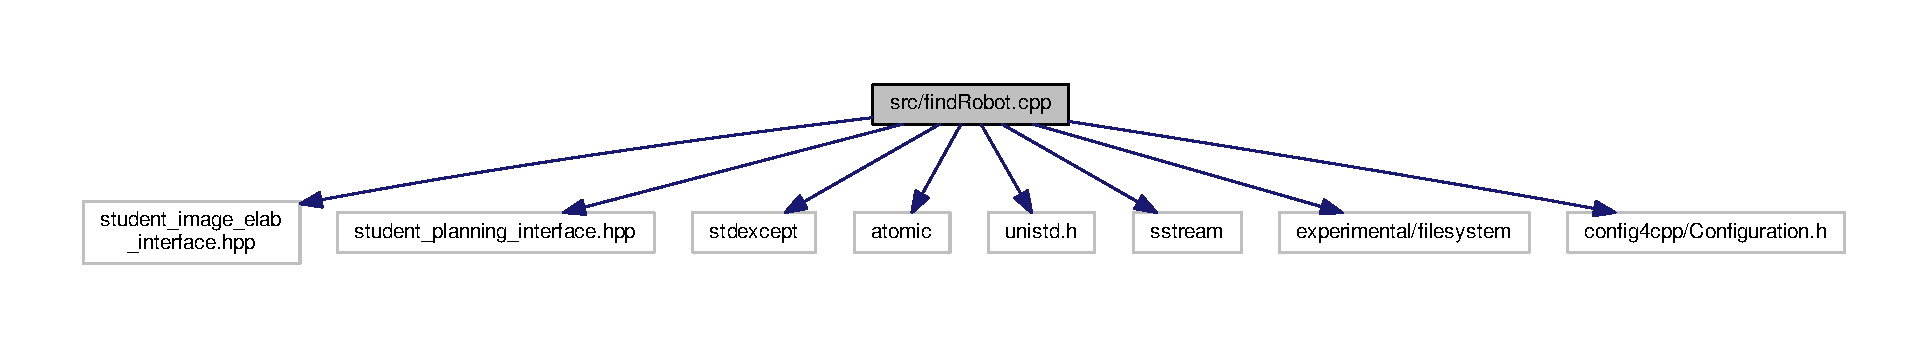
\includegraphics[width=350pt]{findRobot_8cpp__incl}
\end{center}
\end{figure}
\subsection*{Namespaces}
\begin{DoxyCompactItemize}
\item 
 \hyperlink{namespacestudent}{student}
\end{DoxyCompactItemize}
\subsection*{Functions}
\begin{DoxyCompactItemize}
\item 
bool \hyperlink{namespacestudent_afd56b779672a672e15ac45dc927b8a6b}{student\+::find\+Robot} (const cv\+::\+Mat \&img\+\_\+in, const double scale, \hyperlink{utils_8hpp_a18281038c49470960bd8f4d15b893441}{Polygon} \&triangle, double \&x, double \&y, double \&theta, const std\+::string \&config\+\_\+folder)
\begin{DoxyCompactList}\small\item\em find Robot function in student interface \end{DoxyCompactList}\end{DoxyCompactItemize}

\hypertarget{loadImage_8cpp}{}\section{src/load\+Image.cpp File Reference}
\label{loadImage_8cpp}\index{src/load\+Image.\+cpp@{src/load\+Image.\+cpp}}


Contains the implementation of load\+Image Function.  


{\ttfamily \#include \char`\"{}student\+\_\+image\+\_\+elab\+\_\+interface.\+hpp\char`\"{}}\\*
{\ttfamily \#include \char`\"{}student\+\_\+planning\+\_\+interface.\+hpp\char`\"{}}\\*
{\ttfamily \#include $<$stdexcept$>$}\\*
{\ttfamily \#include $<$atomic$>$}\\*
{\ttfamily \#include $<$unistd.\+h$>$}\\*
{\ttfamily \#include $<$sstream$>$}\\*
{\ttfamily \#include $<$experimental/filesystem$>$}\\*
Include dependency graph for load\+Image.\+cpp\+:\nopagebreak
\begin{figure}[H]
\begin{center}
\leavevmode
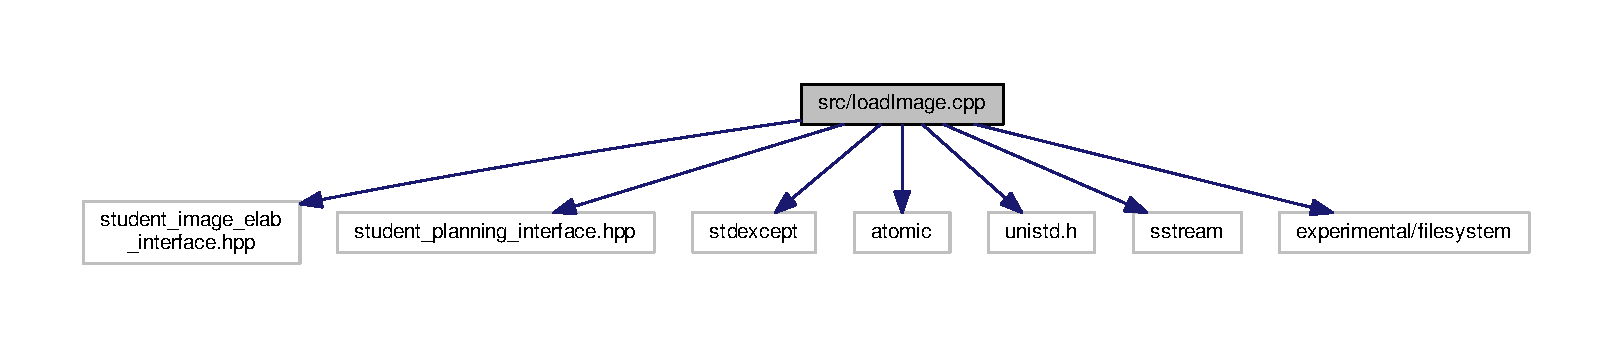
\includegraphics[width=350pt]{loadImage_8cpp__incl}
\end{center}
\end{figure}
\subsection*{Namespaces}
\begin{DoxyCompactItemize}
\item 
 \hyperlink{namespacestudent}{student}
\end{DoxyCompactItemize}
\subsection*{Functions}
\begin{DoxyCompactItemize}
\item 
void \hyperlink{namespacestudent_a3117c968a47bf95f86bdb813a3b64e56}{student\+::load\+Image} (cv\+::\+Mat \&img\+\_\+out, const std\+::string \&config\+\_\+folder)
\begin{DoxyCompactList}\small\item\em load Image function in student interface \end{DoxyCompactList}\end{DoxyCompactItemize}


\subsection{Detailed Description}
Contains the implementation of load\+Image Function. 

\begin{DoxyAuthor}{Author}
Aravind Swaminathan 
\end{DoxyAuthor}
\begin{DoxyDate}{Date}
10-\/\+Jan-\/2020 
\end{DoxyDate}

\hypertarget{planPath_8cpp}{}\section{src/plan\+Path.cpp File Reference}
\label{planPath_8cpp}\index{src/plan\+Path.\+cpp@{src/plan\+Path.\+cpp}}


Contains the implementation of plan\+Path functions.  


{\ttfamily \#include \char`\"{}plan\+Path.\+hpp\char`\"{}}\\*
Include dependency graph for plan\+Path.\+cpp\+:\nopagebreak
\begin{figure}[H]
\begin{center}
\leavevmode
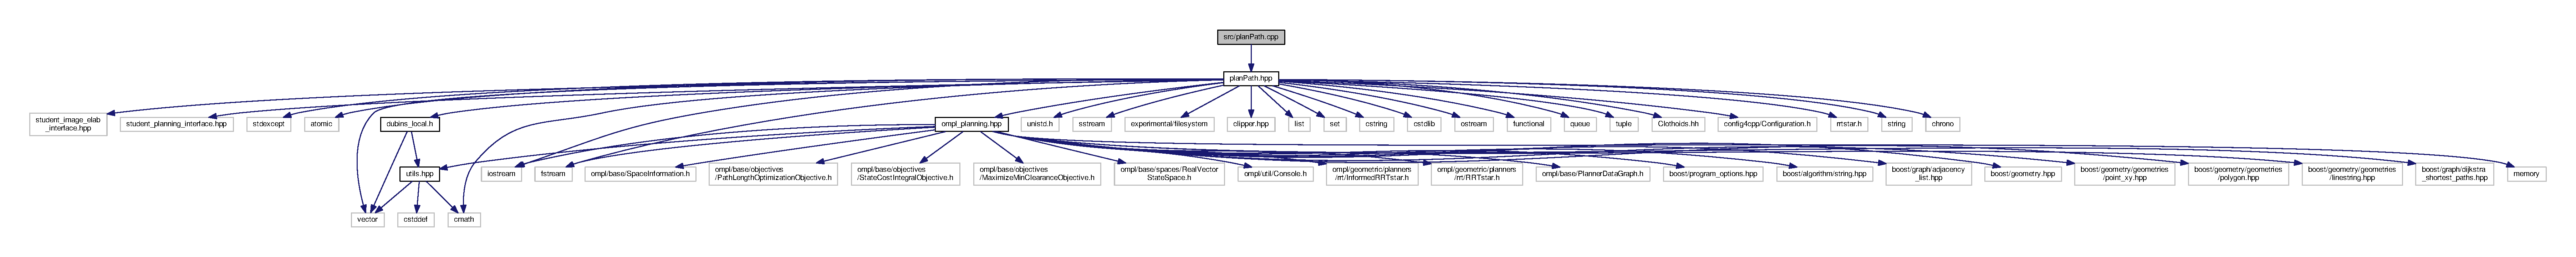
\includegraphics[width=350pt]{planPath_8cpp__incl}
\end{center}
\end{figure}
\subsection*{Classes}
\begin{DoxyCompactItemize}
\item 
class \hyperlink{classconfig__Params__planPath}{config\+\_\+\+Params\+\_\+plan\+Path}
\begin{DoxyCompactList}\small\item\em Class which reads and stores the configuration params related to plan\+Path functions. \end{DoxyCompactList}\end{DoxyCompactItemize}
\subsection*{Namespaces}
\begin{DoxyCompactItemize}
\item 
 \hyperlink{namespacestudent}{student}
\end{DoxyCompactItemize}
\subsection*{Functions}
\begin{DoxyCompactItemize}
\item 
void \hyperlink{planPath_8cpp_a992f985b423725966690e4552becd32a}{print\+\_\+path} (\hyperlink{structPath}{Path} path, \hyperlink{classconfig__Params__planPath}{config\+\_\+\+Params\+\_\+plan\+Path} config\+\_\+params, bool global)
\item 
bool \hyperlink{namespacestudent_a38f4da9abe090023fe1fbf23f75b5b42}{student\+::get\+Curvature} (int step, \hyperlink{structPath}{Path} \&path)
\item 
bool \hyperlink{namespacestudent_abf207b6433d914c39067b7d538c2956c}{student\+::sort\+\_\+pair\+\_\+mission2} (const std\+::pair$<$ int, \hyperlink{utils_8hpp_a18281038c49470960bd8f4d15b893441}{Polygon} $>$ \&a, const std\+::pair$<$ int, \hyperlink{utils_8hpp_a18281038c49470960bd8f4d15b893441}{Polygon} $>$ \&b)
\item 
std\+::vector$<$ \hyperlink{utils_8hpp_a18281038c49470960bd8f4d15b893441}{Polygon} $>$ \hyperlink{namespacestudent_a962ac10ed4e3bf5be63aad206b4fc624}{student\+::obstacle\+Offsetting} (const std\+::vector$<$ \hyperlink{utils_8hpp_a18281038c49470960bd8f4d15b893441}{Polygon} $>$ ob, int offset\+\_\+radius)
\begin{DoxyCompactList}\small\item\em Expand obstacles region to avoid collision. \end{DoxyCompactList}\item 
\hyperlink{utils_8hpp_a18281038c49470960bd8f4d15b893441}{Polygon} \hyperlink{namespacestudent_a4533d2b12567821a0dbb957d0e607fc0}{student\+::resize\+Borders} (const \hyperlink{utils_8hpp_a18281038c49470960bd8f4d15b893441}{Polygon} \&borders, int resize)
\begin{DoxyCompactList}\small\item\em Resize the border for avoiding collision with border. \end{DoxyCompactList}\item 
\hyperlink{utils_8hpp_a18281038c49470960bd8f4d15b893441}{Polygon} \hyperlink{namespacestudent_acf7520b9efd4309e03ec51e8cd7642b0}{student\+::sample\+\_\+borders} (\hyperlink{utils_8hpp_a18281038c49470960bd8f4d15b893441}{Polygon} \&borders)
\begin{DoxyCompactList}\small\item\em Sample the borders with multiple points. \end{DoxyCompactList}\item 
std\+::pair$<$ double, double $>$ \hyperlink{namespacestudent_a4bc9329b042a3a7854a08219559fb863}{student\+::get\+\_\+center} (const \hyperlink{utils_8hpp_a18281038c49470960bd8f4d15b893441}{Polygon} \&poly)
\begin{DoxyCompactList}\small\item\em get centroid of any polygon \end{DoxyCompactList}\item 
bool \hyperlink{namespacestudent_a9c112c915d7bf1e28084673499b7d5ef}{student\+::point\+Inside\+Polygon} (\hyperlink{utils_8hpp_a18281038c49470960bd8f4d15b893441}{Polygon} poly, \hyperlink{structPoint}{Point} pt)
\begin{DoxyCompactList}\small\item\em function to check if a given point is inside polygon \end{DoxyCompactList}\item 
double \hyperlink{namespacestudent_a2da434a66dc725fa325433bb9bd4e989}{student\+::compute\+\_\+angle\+\_\+gate} (\hyperlink{utils_8hpp_a18281038c49470960bd8f4d15b893441}{Polygon} borders, double gateX, double gateY)
\begin{DoxyCompactList}\small\item\em function to compute the gate angle \end{DoxyCompactList}\item 
double \hyperlink{namespacestudent_ac8e0adb0fb2cb218e2410c460af2cae7}{student\+::internal\+\_\+angle} (double angle1, double angle2)
\item 
double \hyperlink{namespacestudent_ac51402ca51fa6c279f88cf560e32b422}{student\+::get\+\_\+angle} (\hyperlink{structPose}{Pose} first, \hyperlink{structPose}{Pose} second, \hyperlink{structPose}{Pose} third)
\begin{DoxyCompactList}\small\item\em function to compute the approach angle between two nodes \end{DoxyCompactList}\item 
bool \hyperlink{namespacestudent_a7e23765e95f85572437c4f8bc2bc6d6e}{student\+::check\+\_\+collison\+\_\+with\+\_\+borders\+\_\+and\+\_\+obstacles} (\hyperlink{structPath}{Path} path, \hyperlink{utils_8hpp_a18281038c49470960bd8f4d15b893441}{Polygon} borders, \hyperlink{utils_8hpp_a18281038c49470960bd8f4d15b893441}{Polygon} sampled\+\_\+borders, std\+::vector$<$ \hyperlink{utils_8hpp_a18281038c49470960bd8f4d15b893441}{Polygon} $>$ obstacle\+\_\+list, std\+::vector$<$ double $>$ obs\+\_\+radius, std\+::vector$<$ \hyperlink{structPoint}{Point} $>$ obs\+\_\+center)
\begin{DoxyCompactList}\small\item\em function to check if the generated path is colliding with borders and obstacles \end{DoxyCompactList}\item 
void \hyperlink{namespacestudent_ae985c265d91c51e3afdc782c70964ecd}{student\+::\+R\+R\+T\+\_\+\+Star} (const float x, const float y, const float theta, \hyperlink{structPath}{Path} \&path, std\+::vector$<$ \hyperlink{structPoint}{Point} $>$ \&local\+Goals, const \hyperlink{utils_8hpp_a18281038c49470960bd8f4d15b893441}{Polygon} \&borders, \hyperlink{utils_8hpp_a18281038c49470960bd8f4d15b893441}{Polygon} \&sampled\+\_\+borders, const std\+::vector$<$ \hyperlink{utils_8hpp_a18281038c49470960bd8f4d15b893441}{Polygon} $>$ \&obstacle\+\_\+list, std\+::vector$<$ double $>$ obs\+\_\+radius, std\+::vector$<$ \hyperlink{structPoint}{Point} $>$ obs\+\_\+center, \hyperlink{classconfig__Params__planPath}{config\+\_\+\+Params\+\_\+plan\+Path} config\+\_\+params)
\begin{DoxyCompactList}\small\item\em implmentation of R\+RT Star function \end{DoxyCompactList}\item 
void \hyperlink{namespacestudent_ab8f6c07df2df619bef2b28d6f7ebcac7}{student\+::\+R\+R\+T\+\_\+\+Star\+\_\+ompl} (const float x, const float y, const float theta, \hyperlink{structPath}{Path} \&path, std\+::vector$<$ \hyperlink{structPoint}{Point} $>$ \&local\+Goals, const \hyperlink{utils_8hpp_a18281038c49470960bd8f4d15b893441}{Polygon} \&borders, \hyperlink{utils_8hpp_a18281038c49470960bd8f4d15b893441}{Polygon} \&sampled\+\_\+borders, const std\+::vector$<$ \hyperlink{utils_8hpp_a18281038c49470960bd8f4d15b893441}{Polygon} $>$ \&obstacle\+\_\+list, std\+::vector$<$ double $>$ obs\+\_\+radius, std\+::vector$<$ \hyperlink{structPoint}{Point} $>$ obs\+\_\+center, \hyperlink{classconfig__Params__planPath}{config\+\_\+\+Params\+\_\+plan\+Path} config\+\_\+params)
\begin{DoxyCompactList}\small\item\em implmentation of R\+RT Star function using O\+M\+PL library \end{DoxyCompactList}\item 
std\+::vector$<$ \hyperlink{structPoint}{Point} $>$ \hyperlink{namespacestudent_a6d911d7d7118f5393eeb575e0e76cdf6}{student\+::compute\+\_\+vicitim\+\_\+mission2} (const float x, const float y, const float theta, const \hyperlink{utils_8hpp_a18281038c49470960bd8f4d15b893441}{Polygon} \&borders, const std\+::vector$<$ \hyperlink{utils_8hpp_a18281038c49470960bd8f4d15b893441}{Polygon} $>$ \&obstacle\+\_\+list, std\+::pair$<$ double, double $>$ gate\+Center, std\+::vector$<$ std\+::pair$<$ int, \hyperlink{utils_8hpp_a18281038c49470960bd8f4d15b893441}{Polygon} $>$$>$ victim\+\_\+list, \hyperlink{classconfig__Params__planPath}{config\+\_\+\+Params\+\_\+plan\+Path} config\+\_\+params)
\begin{DoxyCompactList}\small\item\em implmentation of Mission targets for mision 2 \end{DoxyCompactList}\item 
bool \hyperlink{namespacestudent_acfe62076a49d23bb083f2f880fd24c77}{student\+::plan\+Path} (const \hyperlink{utils_8hpp_a18281038c49470960bd8f4d15b893441}{Polygon} \&borders, const std\+::vector$<$ \hyperlink{utils_8hpp_a18281038c49470960bd8f4d15b893441}{Polygon} $>$ \&obstacle\+\_\+list, const std\+::vector$<$ std\+::pair$<$ int, \hyperlink{utils_8hpp_a18281038c49470960bd8f4d15b893441}{Polygon} $>$$>$ \&victim\+\_\+list, const \hyperlink{utils_8hpp_a18281038c49470960bd8f4d15b893441}{Polygon} \&gate, const float x, const float y, const float theta, \hyperlink{structPath}{Path} \&path, const std\+::string \&config\+\_\+folder)
\begin{DoxyCompactList}\small\item\em Plan a safe and fast path in the arena. \end{DoxyCompactList}\end{DoxyCompactItemize}


\subsection{Detailed Description}
Contains the implementation of plan\+Path functions. 

\begin{DoxyAuthor}{Author}
Aravind Swaminathan 
\end{DoxyAuthor}
\begin{DoxyDate}{Date}
10-\/\+Jan-\/2020 
\end{DoxyDate}


\subsection{Function Documentation}
\index{plan\+Path.\+cpp@{plan\+Path.\+cpp}!print\+\_\+path@{print\+\_\+path}}
\index{print\+\_\+path@{print\+\_\+path}!plan\+Path.\+cpp@{plan\+Path.\+cpp}}
\subsubsection[{\texorpdfstring{print\+\_\+path(\+Path path, config\+\_\+\+Params\+\_\+plan\+Path config\+\_\+params, bool global)}{print_path(Path path, config_Params_planPath config_params, bool global)}}]{\setlength{\rightskip}{0pt plus 5cm}void print\+\_\+path (
\begin{DoxyParamCaption}
\item[{{\bf Path}}]{path, }
\item[{{\bf config\+\_\+\+Params\+\_\+plan\+Path}}]{config\+\_\+params, }
\item[{bool}]{global}
\end{DoxyParamCaption}
)}\hypertarget{planPath_8cpp_a992f985b423725966690e4552becd32a}{}\label{planPath_8cpp_a992f985b423725966690e4552becd32a}
Function to store the path information computed to a file. Save location hardcoded 
\begin{DoxyParams}{Parameters}
{\em x} & -\/ \hyperlink{structPath}{Path} struct \\
\hline
\end{DoxyParams}
\begin{DoxyReturn}{Returns}
None 
\end{DoxyReturn}

\hypertarget{processMap_8cpp}{}\section{src/process\+Map.cpp File Reference}
\label{processMap_8cpp}\index{src/process\+Map.\+cpp@{src/process\+Map.\+cpp}}


Contains the implementation of Obstacle detection, gate detecton , victm detection and victim recognition.  


{\ttfamily \#include \char`\"{}student\+\_\+image\+\_\+elab\+\_\+interface.\+hpp\char`\"{}}\\*
{\ttfamily \#include \char`\"{}student\+\_\+planning\+\_\+interface.\+hpp\char`\"{}}\\*
{\ttfamily \#include $<$stdexcept$>$}\\*
{\ttfamily \#include $<$atomic$>$}\\*
{\ttfamily \#include $<$unistd.\+h$>$}\\*
{\ttfamily \#include $<$sstream$>$}\\*
{\ttfamily \#include $<$experimental/filesystem$>$}\\*
{\ttfamily \#include $<$tesseract/baseapi.\+h$>$}\\*
{\ttfamily \#include $<$leptonica/allheaders.\+h$>$}\\*
{\ttfamily \#include $<$config4cpp/\+Configuration.\+h$>$}\\*
Include dependency graph for process\+Map.\+cpp\+:\nopagebreak
\begin{figure}[H]
\begin{center}
\leavevmode
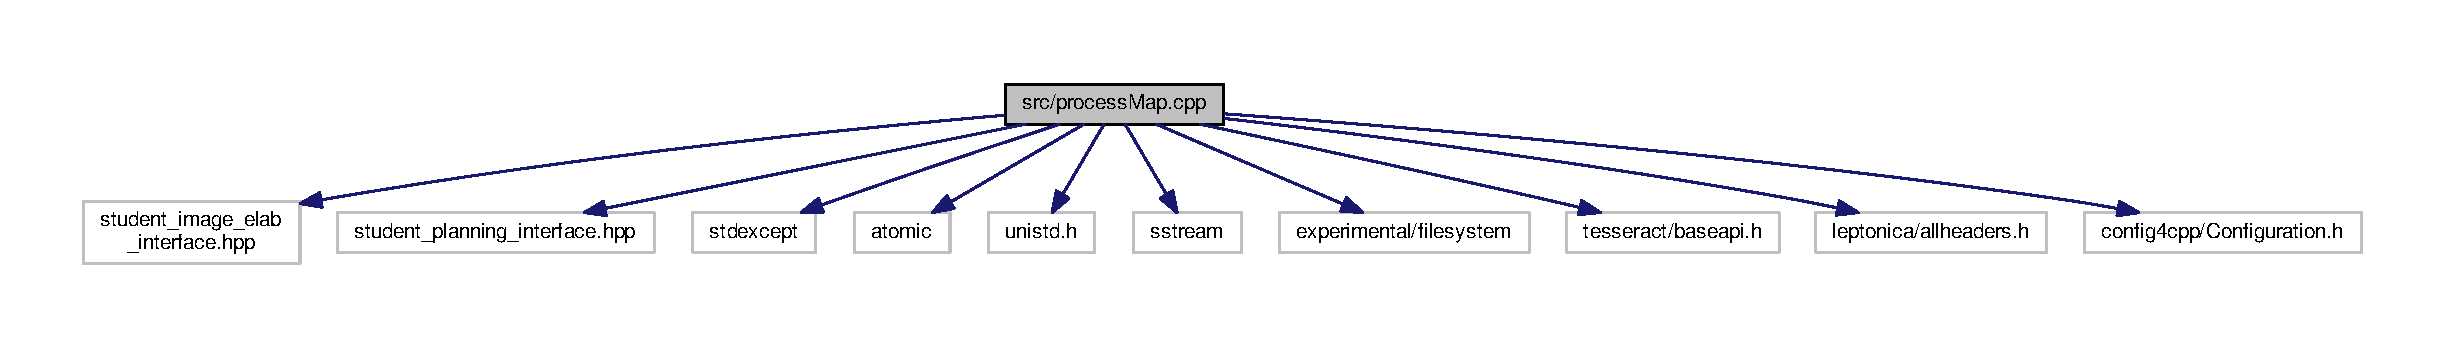
\includegraphics[width=350pt]{processMap_8cpp__incl}
\end{center}
\end{figure}
\subsection*{Classes}
\begin{DoxyCompactItemize}
\item 
class \hyperlink{classconfig__Params__ProcessMap}{config\+\_\+\+Params\+\_\+\+Process\+Map}
\begin{DoxyCompactList}\small\item\em Class which reads and stores the configuration params related to process\+Map functions. \end{DoxyCompactList}\end{DoxyCompactItemize}
\subsection*{Namespaces}
\begin{DoxyCompactItemize}
\item 
 \hyperlink{namespacestudent}{student}
\end{DoxyCompactItemize}
\subsection*{Functions}
\begin{DoxyCompactItemize}
\item 
bool \hyperlink{namespacestudent_a5ae5c8a6b753e8c2f86e2a6f70c44faf}{student\+::sort\+\_\+pair} (const std\+::pair$<$ int, \hyperlink{utils_8hpp_a18281038c49470960bd8f4d15b893441}{Polygon} $>$ \&a, const std\+::pair$<$ int, \hyperlink{utils_8hpp_a18281038c49470960bd8f4d15b893441}{Polygon} $>$ \&b)
\item 
bool \hyperlink{namespacestudent_a18b392b6e41e30b0e80eadf53d6d890b}{student\+::process\+Obstacles} (const cv\+::\+Mat \&hsv\+\_\+img, const double scale, std\+::vector$<$ \hyperlink{utils_8hpp_a18281038c49470960bd8f4d15b893441}{Polygon} $>$ \&obstacle\+\_\+list, \hyperlink{classconfig__Params__ProcessMap}{config\+\_\+\+Params\+\_\+\+Process\+Map} config\+\_\+params)
\begin{DoxyCompactList}\small\item\em Obstacle detection function. \end{DoxyCompactList}\item 
bool \hyperlink{namespacestudent_abfb444a179b51148e9ad476a016f8fe3}{student\+::process\+Gate} (const cv\+::\+Mat \&hsv\+\_\+img, const double scale, \hyperlink{utils_8hpp_a18281038c49470960bd8f4d15b893441}{Polygon} \&gate, \hyperlink{classconfig__Params__ProcessMap}{config\+\_\+\+Params\+\_\+\+Process\+Map} config\+\_\+params)
\begin{DoxyCompactList}\small\item\em gate detection function \end{DoxyCompactList}\item 
int \hyperlink{namespacestudent_a4d19daafa227fb7503f8ff4111243d4d}{student\+::get\+\_\+victim\+\_\+id} (cv\+::\+Rect bounding\+Rect, cv\+::\+Mat img, \hyperlink{classconfig__Params__ProcessMap}{config\+\_\+\+Params\+\_\+\+Process\+Map} config\+\_\+params)
\begin{DoxyCompactList}\small\item\em Function to get victim ID. \end{DoxyCompactList}\item 
bool \hyperlink{namespacestudent_a6dd3cda22103f4e0c2ddb32cc68789c7}{student\+::process\+Victims} (const cv\+::\+Mat \&hsv\+\_\+img, const double scale, std\+::vector$<$ std\+::pair$<$ int, \hyperlink{utils_8hpp_a18281038c49470960bd8f4d15b893441}{Polygon} $>$$>$ \&victim\+\_\+list, \hyperlink{classconfig__Params__ProcessMap}{config\+\_\+\+Params\+\_\+\+Process\+Map} config\+\_\+params)
\begin{DoxyCompactList}\small\item\em Victim detection function along with digit recognition call. \end{DoxyCompactList}\item 
bool \hyperlink{namespacestudent_a153a17ef667d7c10b8f33d815b9bc1bc}{student\+::process\+Map} (const cv\+::\+Mat \&img\+\_\+in, const double scale, std\+::vector$<$ \hyperlink{utils_8hpp_a18281038c49470960bd8f4d15b893441}{Polygon} $>$ \&obstacle\+\_\+list, std\+::vector$<$ std\+::pair$<$ int, \hyperlink{utils_8hpp_a18281038c49470960bd8f4d15b893441}{Polygon} $>$$>$ \&victim\+\_\+list, \hyperlink{utils_8hpp_a18281038c49470960bd8f4d15b893441}{Polygon} \&gate, const std\+::string \&config\+\_\+folder)
\begin{DoxyCompactList}\small\item\em Main function to call process\+Obstacles, process\+Gate and process\+Victims. \end{DoxyCompactList}\end{DoxyCompactItemize}
\subsection*{Variables}
\begin{DoxyCompactItemize}
\item 
cv\+::\+Mat \hyperlink{namespacestudent_aba626c3c54f4003c9c06f7fea899efc2}{student\+::debug\+\_\+image}
\end{DoxyCompactItemize}


\subsection{Detailed Description}
Contains the implementation of Obstacle detection, gate detecton , victm detection and victim recognition. 

\begin{DoxyAuthor}{Author}
Aravind Swaminathan 
\end{DoxyAuthor}
\begin{DoxyDate}{Date}
10-\/\+Jan-\/2020 
\end{DoxyDate}

\hypertarget{obstacles_8cpp}{}\section{src/\+R\+R\+T\+Star/obstacles.cpp File Reference}
\label{obstacles_8cpp}\index{src/\+R\+R\+T\+Star/obstacles.\+cpp@{src/\+R\+R\+T\+Star/obstacles.\+cpp}}
{\ttfamily \#include \char`\"{}obstacles.\+h\char`\"{}}\\*
{\ttfamily \#include $<$iostream$>$}\\*
Include dependency graph for obstacles.\+cpp\+:\nopagebreak
\begin{figure}[H]
\begin{center}
\leavevmode
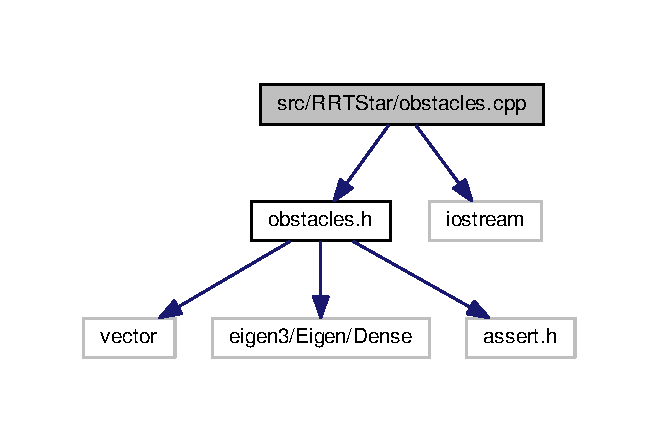
\includegraphics[width=316pt]{obstacles_8cpp__incl}
\end{center}
\end{figure}
\subsection*{Functions}
\begin{DoxyCompactItemize}
\item 
bool \hyperlink{obstacles_8cpp_a7de48b8f590f5e707e18dedf61f4cccd}{is\+Inside} (int circle\+\_\+x, int circle\+\_\+y, int rad, int x, int y)
\begin{DoxyCompactList}\small\item\em Check if point is inside the obstacle circle. \end{DoxyCompactList}\item 
bool \hyperlink{obstacles_8cpp_a903e54621bae3cecb0e8e292c55e91e0}{check\+Collision} (int a, int b, int c, int x, int y, int radius)
\end{DoxyCompactItemize}


\subsection{Function Documentation}
\index{obstacles.\+cpp@{obstacles.\+cpp}!check\+Collision@{check\+Collision}}
\index{check\+Collision@{check\+Collision}!obstacles.\+cpp@{obstacles.\+cpp}}
\subsubsection[{\texorpdfstring{check\+Collision(int a, int b, int c, int x, int y, int radius)}{checkCollision(int a, int b, int c, int x, int y, int radius)}}]{\setlength{\rightskip}{0pt plus 5cm}bool check\+Collision (
\begin{DoxyParamCaption}
\item[{int}]{a, }
\item[{int}]{b, }
\item[{int}]{c, }
\item[{int}]{x, }
\item[{int}]{y, }
\item[{int}]{radius}
\end{DoxyParamCaption}
)}\hypertarget{obstacles_8cpp_a903e54621bae3cecb0e8e292c55e91e0}{}\label{obstacles_8cpp_a903e54621bae3cecb0e8e292c55e91e0}
\index{obstacles.\+cpp@{obstacles.\+cpp}!is\+Inside@{is\+Inside}}
\index{is\+Inside@{is\+Inside}!obstacles.\+cpp@{obstacles.\+cpp}}
\subsubsection[{\texorpdfstring{is\+Inside(int circle\+\_\+x, int circle\+\_\+y, int rad, int x, int y)}{isInside(int circle_x, int circle_y, int rad, int x, int y)}}]{\setlength{\rightskip}{0pt plus 5cm}bool is\+Inside (
\begin{DoxyParamCaption}
\item[{int}]{circle\+\_\+x, }
\item[{int}]{circle\+\_\+y, }
\item[{int}]{rad, }
\item[{int}]{x, }
\item[{int}]{y}
\end{DoxyParamCaption}
)}\hypertarget{obstacles_8cpp_a7de48b8f590f5e707e18dedf61f4cccd}{}\label{obstacles_8cpp_a7de48b8f590f5e707e18dedf61f4cccd}


Check if point is inside the obstacle circle. 


\begin{DoxyParams}{Parameters}
{\em radius} & \\
\hline
{\em second\+Point} & \\
\hline
\end{DoxyParams}

\hypertarget{obstacles_8h}{}\section{src/\+R\+R\+T\+Star/obstacles.h File Reference}
\label{obstacles_8h}\index{src/\+R\+R\+T\+Star/obstacles.\+h@{src/\+R\+R\+T\+Star/obstacles.\+h}}


Contains the declaration of Obstacles class.  


{\ttfamily \#include $<$vector$>$}\\*
{\ttfamily \#include $<$eigen3/\+Eigen/\+Dense$>$}\\*
{\ttfamily \#include $<$assert.\+h$>$}\\*
Include dependency graph for obstacles.\+h\+:\nopagebreak
\begin{figure}[H]
\begin{center}
\leavevmode
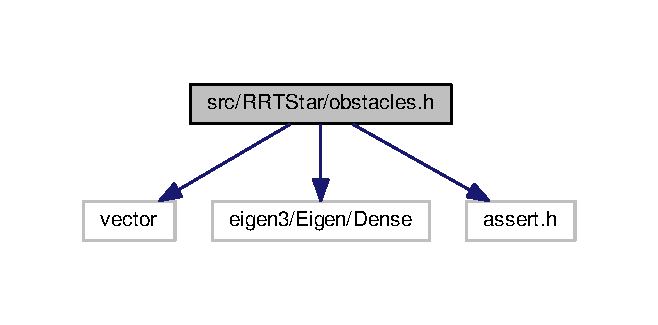
\includegraphics[width=316pt]{obstacles_8h__incl}
\end{center}
\end{figure}
This graph shows which files directly or indirectly include this file\+:\nopagebreak
\begin{figure}[H]
\begin{center}
\leavevmode
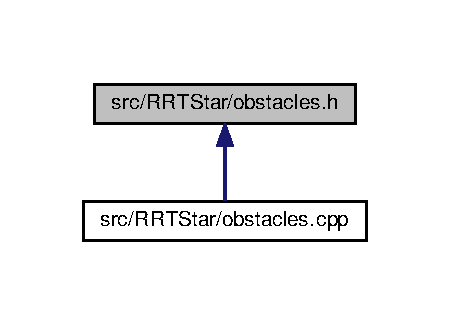
\includegraphics[width=350pt]{obstacles_8h__dep__incl}
\end{center}
\end{figure}
\subsection*{Classes}
\begin{DoxyCompactItemize}
\item 
class \hyperlink{classRRTObstacles}{R\+R\+T\+Obstacles}
\begin{DoxyCompactList}\small\item\em Obstacles class for R\+R\+T$\ast$ Star Implementation. \end{DoxyCompactList}\end{DoxyCompactItemize}


\subsection{Detailed Description}
Contains the declaration of Obstacles class. 

\begin{DoxyAuthor}{Author}
Aravind Swaminathan 
\end{DoxyAuthor}
\begin{DoxyDate}{Date}
10-\/\+Jan-\/2020 
\end{DoxyDate}

\hypertarget{rrtstar_8cpp}{}\section{src/\+R\+R\+T\+Star/rrtstar.cpp File Reference}
\label{rrtstar_8cpp}\index{src/\+R\+R\+T\+Star/rrtstar.\+cpp@{src/\+R\+R\+T\+Star/rrtstar.\+cpp}}
{\ttfamily \#include \char`\"{}rrtstar.\+h\char`\"{}}\\*
Include dependency graph for rrtstar.\+cpp\+:\nopagebreak
\begin{figure}[H]
\begin{center}
\leavevmode
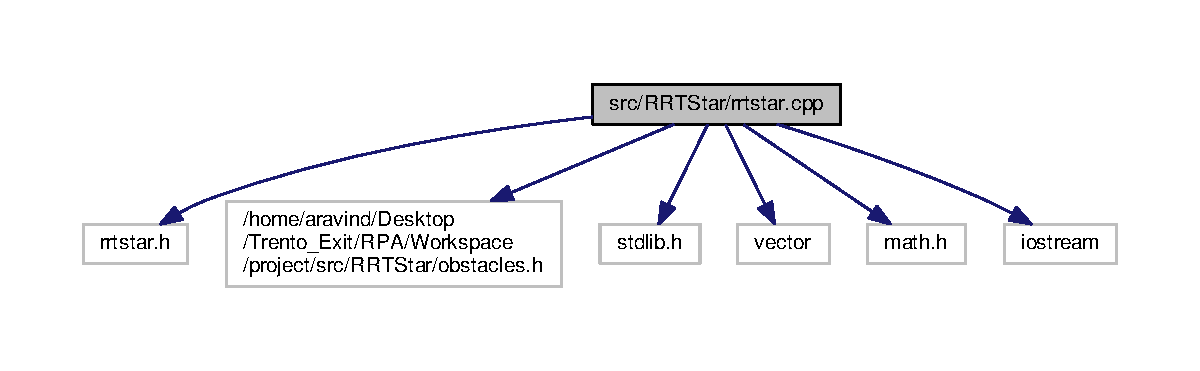
\includegraphics[width=350pt]{rrtstar_8cpp__incl}
\end{center}
\end{figure}

\hypertarget{rrtstar_8h}{}\section{src/\+R\+R\+T\+Star/rrtstar.h File Reference}
\label{rrtstar_8h}\index{src/\+R\+R\+T\+Star/rrtstar.\+h@{src/\+R\+R\+T\+Star/rrtstar.\+h}}


Contains the declation of R\+R\+T$\ast$ class and R\+R\+T$\ast$ \hyperlink{structNode}{Node}.  


{\ttfamily \#include \char`\"{}obstacles.\+h\char`\"{}}\\*
{\ttfamily \#include $<$stdlib.\+h$>$}\\*
{\ttfamily \#include $<$vector$>$}\\*
{\ttfamily \#include $<$math.\+h$>$}\\*
{\ttfamily \#include $<$iostream$>$}\\*
Include dependency graph for rrtstar.\+h\+:\nopagebreak
\begin{figure}[H]
\begin{center}
\leavevmode
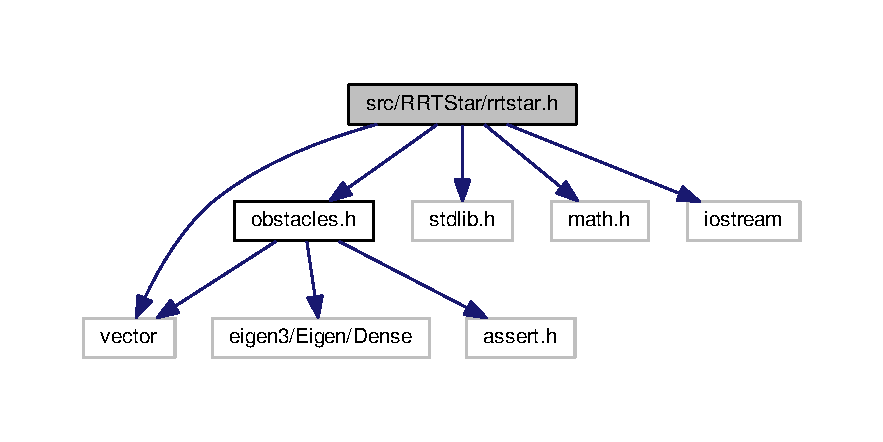
\includegraphics[width=350pt]{rrtstar_8h__incl}
\end{center}
\end{figure}
This graph shows which files directly or indirectly include this file\+:\nopagebreak
\begin{figure}[H]
\begin{center}
\leavevmode
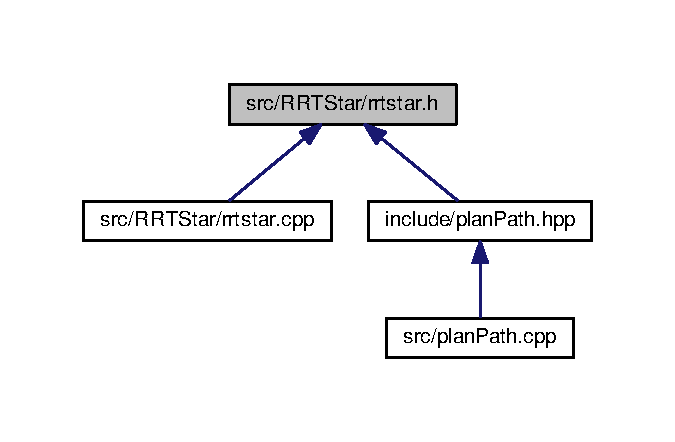
\includegraphics[width=324pt]{rrtstar_8h__dep__incl}
\end{center}
\end{figure}
\subsection*{Classes}
\begin{DoxyCompactItemize}
\item 
struct \hyperlink{structNode}{Node}
\begin{DoxyCompactList}\small\item\em R\+R\+T$\ast$ \hyperlink{structNode}{Node} strut. \end{DoxyCompactList}\item 
class \hyperlink{classRRTSTAR}{R\+R\+T\+S\+T\+AR}
\begin{DoxyCompactList}\small\item\em R\+R\+T\+Star Class. \end{DoxyCompactList}\end{DoxyCompactItemize}


\subsection{Detailed Description}
Contains the declation of R\+R\+T$\ast$ class and R\+R\+T$\ast$ \hyperlink{structNode}{Node}. 

\begin{DoxyAuthor}{Author}
Aravind Swaminathan 
\end{DoxyAuthor}
\begin{DoxyDate}{Date}
10-\/\+Jan-\/2020 
\end{DoxyDate}

\hypertarget{student__interface_8cpp}{}\section{src/student\+\_\+interface.cpp File Reference}
\label{student__interface_8cpp}\index{src/student\+\_\+interface.\+cpp@{src/student\+\_\+interface.\+cpp}}


Contains the implementation of generic\+Image\+Listener Function.\+Other functions are moved out in other files.  


{\ttfamily \#include \char`\"{}student\+\_\+image\+\_\+elab\+\_\+interface.\+hpp\char`\"{}}\\*
{\ttfamily \#include \char`\"{}student\+\_\+planning\+\_\+interface.\+hpp\char`\"{}}\\*
{\ttfamily \#include $<$stdexcept$>$}\\*
{\ttfamily \#include $<$atomic$>$}\\*
{\ttfamily \#include $<$unistd.\+h$>$}\\*
{\ttfamily \#include $<$sstream$>$}\\*
{\ttfamily \#include $<$experimental/filesystem$>$}\\*
Include dependency graph for student\+\_\+interface.\+cpp\+:\nopagebreak
\begin{figure}[H]
\begin{center}
\leavevmode
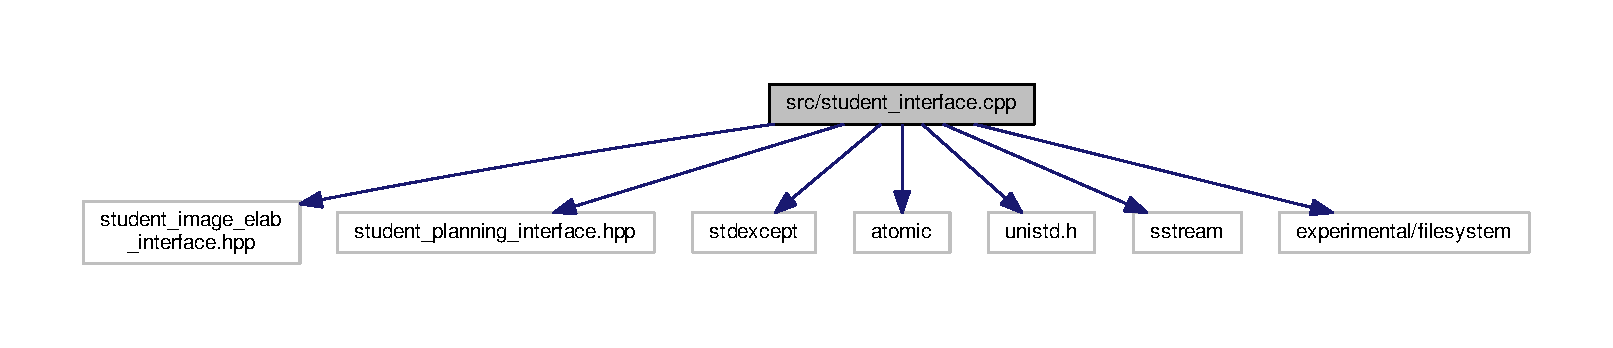
\includegraphics[width=350pt]{student__interface_8cpp__incl}
\end{center}
\end{figure}
\subsection*{Namespaces}
\begin{DoxyCompactItemize}
\item 
 \hyperlink{namespacestudent}{student}
\end{DoxyCompactItemize}
\subsection*{Functions}
\begin{DoxyCompactItemize}
\item 
void \hyperlink{namespacestudent_a3b726e7af03a643c06dcde23057a82ea}{student\+::generic\+Image\+Listener} (const cv\+::\+Mat \&img\+\_\+in, std\+::string topic, const std\+::string \&config\+\_\+folder)
\begin{DoxyCompactList}\small\item\em Function to save images for intrinsic calibration. \end{DoxyCompactList}\end{DoxyCompactItemize}


\subsection{Detailed Description}
Contains the implementation of generic\+Image\+Listener Function.\+Other functions are moved out in other files. 

\begin{DoxyAuthor}{Author}
Aravind Swaminathan 
\end{DoxyAuthor}
\begin{DoxyDate}{Date}
10-\/\+Jan-\/2020 
\end{DoxyDate}

\hypertarget{utils_8hpp}{}\section{/home/aravind/\+Desktop/\+Trento\+\_\+\+Exit/\+R\+P\+A/\+Workspace/simulator/src/9\+\_\+project\+\_\+interface/include/utils.hpp File Reference}
\label{utils_8hpp}\index{/home/aravind/\+Desktop/\+Trento\+\_\+\+Exit/\+R\+P\+A/\+Workspace/simulator/src/9\+\_\+project\+\_\+interface/include/utils.\+hpp@{/home/aravind/\+Desktop/\+Trento\+\_\+\+Exit/\+R\+P\+A/\+Workspace/simulator/src/9\+\_\+project\+\_\+interface/include/utils.\+hpp}}
{\ttfamily \#include $<$vector$>$}\\*
{\ttfamily \#include $<$cmath$>$}\\*
{\ttfamily \#include $<$cstddef$>$}\\*
Include dependency graph for utils.\+hpp\+:\nopagebreak
\begin{figure}[H]
\begin{center}
\leavevmode
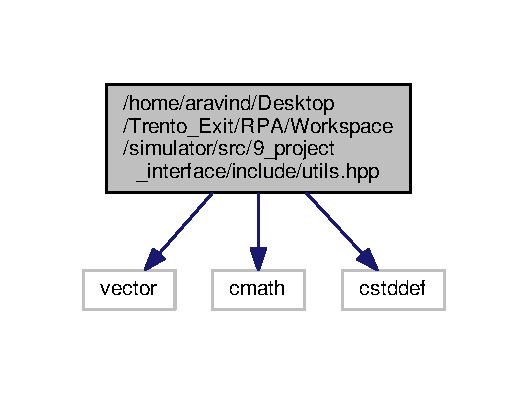
\includegraphics[width=254pt]{utils_8hpp__incl}
\end{center}
\end{figure}
This graph shows which files directly or indirectly include this file\+:\nopagebreak
\begin{figure}[H]
\begin{center}
\leavevmode
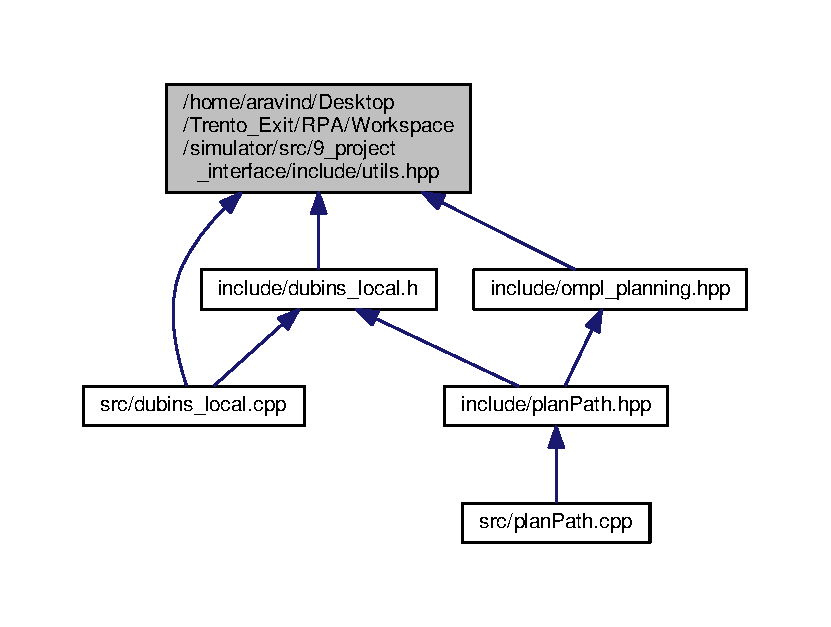
\includegraphics[width=350pt]{utils_8hpp__dep__incl}
\end{center}
\end{figure}
\subsection*{Classes}
\begin{DoxyCompactItemize}
\item 
struct \hyperlink{structPose}{Pose}
\begin{DoxyCompactList}\small\item\em A configuration of the robot along the path, represented by x, y, orientation and curvature. \end{DoxyCompactList}\item 
struct \hyperlink{structPath}{Path}
\begin{DoxyCompactList}\small\item\em A sequence of sampled robot configurations composing a (discretization of the) path. \end{DoxyCompactList}\item 
struct \hyperlink{structPoint}{Point}
\begin{DoxyCompactList}\small\item\em \hyperlink{structPoint}{Point} in given space. \end{DoxyCompactList}\end{DoxyCompactItemize}
\subsection*{Typedefs}
\begin{DoxyCompactItemize}
\item 
typedef std\+::vector$<$ \hyperlink{structPoint}{Point} $>$ \hyperlink{utils_8hpp_a18281038c49470960bd8f4d15b893441}{Polygon}
\begin{DoxyCompactList}\small\item\em Polygon(which is a representation of multiple points) \end{DoxyCompactList}\end{DoxyCompactItemize}


\subsection{Typedef Documentation}
\index{utils.\+hpp@{utils.\+hpp}!Polygon@{Polygon}}
\index{Polygon@{Polygon}!utils.\+hpp@{utils.\+hpp}}
\subsubsection[{\texorpdfstring{Polygon}{Polygon}}]{\setlength{\rightskip}{0pt plus 5cm}typedef std\+::vector$<${\bf Point}$>$ {\bf Polygon}}\hypertarget{utils_8hpp_a18281038c49470960bd8f4d15b893441}{}\label{utils_8hpp_a18281038c49470960bd8f4d15b893441}


Polygon(which is a representation of multiple points) 


%--- End generated contents ---

% Index
\backmatter
\newpage
\phantomsection
\clearemptydoublepage
\addcontentsline{toc}{chapter}{Index}
\printindex

\end{document}
